\documentclass[
  final,
  pagePreset=largepage,
  babelLanguage=portuguese,
  %showtrims,% necessary for print b/c of the images.
  %webversion,
]{anecdote}

\usepackage{local}

% TODO: check Sangha Words
% FIXME: Nikaya
% FIXME: ``` '''

%% Details of the book
%% ===================

\title{Travessia na Floresta}
\subtitle{}
\author{Ajahn Mudito}
\publisher{Amaravati Publications}
\date{2016-02-01}
\editionInfo{}
\ISBN{978-1-78432-047-8}

%% === Load further packages ===

%% === Hyphenation exceptions and corrections ===

% \hyphenation{}

\begin{document}

\ifwebversion
\webcover{%
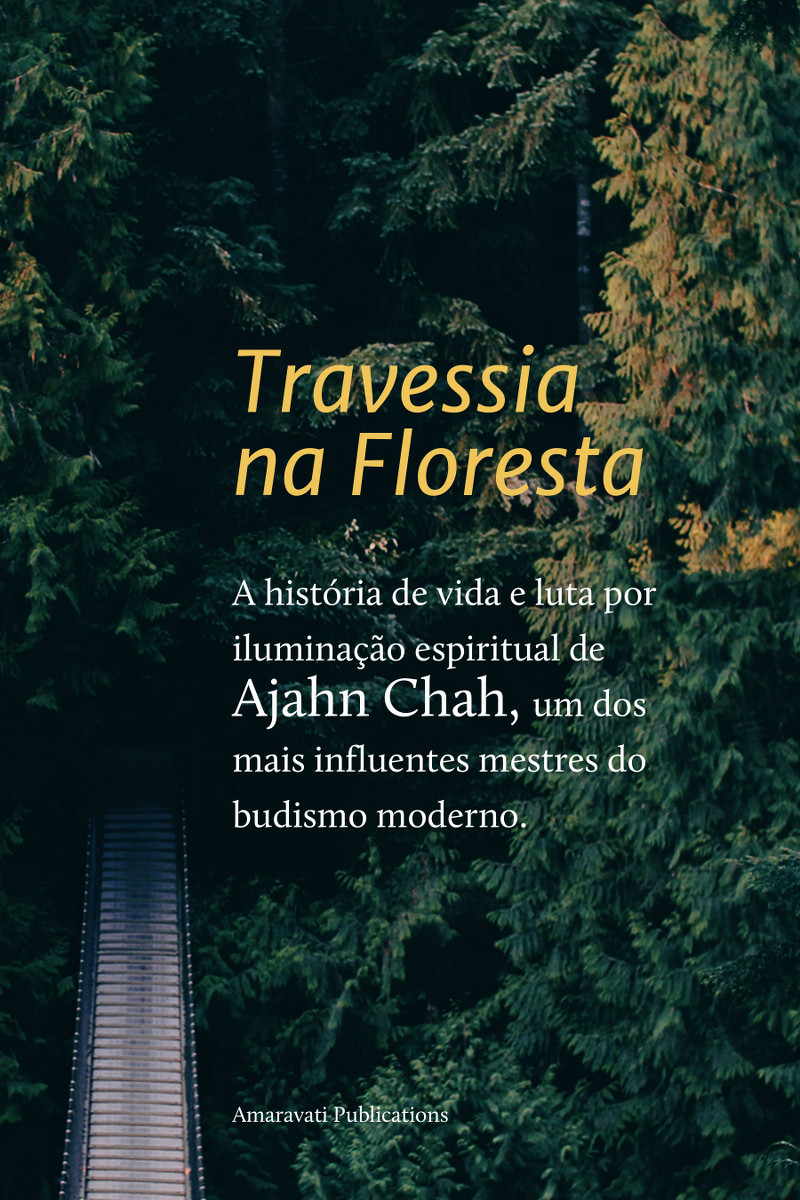
\includegraphics[height=\paperheight]{./webcover.jpg}%
}
\fi

\frontmatter

\cleartorecto
\thispagestyle{empty}
\vspace*{5em}
\newlength\titleLength
\newlength\xheight

{\centering

\settowidth{\titleLength}{%
  {\Large\chapterTitleFont\scshape\MakeLowercase{\thetitle}}%
}

{\Large\chapterTitleFont\itshape \thetitle}\\[0.3\baselineskip]
\setlength{\xheight}{\heightof{X}}
\raisebox{0.5\xheight}{\color[gray]{0.4}\rule{\titleLength}{0.1pt}}\\[0.3\baselineskip]
{\itshape A história de vida e luta por iluminação\\
espiritual de Ajahn Chah (Prah Bodhiññā Thera)}

\vfill

Copyright \copyright\ \thePublisher\ 2016

\vspace*{5em}

}




\cleartoverso
\thispagestyle{empty}

{\copyrightsize
\centering
\setlength{\parindent}{0pt}%
\setlength{\parskip}{0.8\baselineskip}%

\thetitle\\
by \theauthor

Published by \thePublisher

ISBN \theISBN

Copyright \copyright\ \thePublisher\ 2016

\vfill

{\footnotesize

\textit{Sabbadānaṃ dhammadānaṃ jinati}\\
‘The gift of Dhamma surpasses all other gifts.’

This work is licensed under a Creative Commons\\
Attribution-NonCommercial-NoDerivatives 4.0 International~License.

Produced with the \LaTeX\ typesetting system, set in Gentium, Alegreya~Sans and Crimson~Roman.

\theEditionInfo

}}

% TODO
%
%Amaravati Monastério Budista
%
%Great Gaddesden, Hertfordshire, HP1 3BZ
%
%Reino Unido,
%
%www.amaravati.org
%
%Amaravati Publications é parte do ``The English Sangha Trust'', uma
%instituição de caridade registrada no Reino Unido com o número 231310.
%
%Publicado pela primeira vez por Amaravati Publications 2015.
%
%ISBN 978-1-78432-048-5
%
%Imagem de capa de autoria de Nick Sheerbart, licenciada sob Public
%Domain Dedication (http://creativecommons.org/publicdomain/zero/1.0/).
%Para mais informações sobre o autor, visite
%http://www.nick-scheerbart.com/
%
%Este livro é feito disponível como uma oferta de Darma. A sua impressão
%tornou-se possível devido à fé, empenho e generosidade de indivíduos que
%desejam partilhar a sabedoria deste conteúdo com todos aqueles que
%estiverem interessados. Este ato de oferecer gratuitamente é, em parte,
%o que torna esta uma ``publicação de Darma'', um livro baseado em
%valores espirituais. É proibido vender este livro, sob qualquer formato,
%ou usá-lo para fins comerciais.
%
%Se deseja contribuir para que publicações como esta continuem
%disponíveis, você pode fazer sua contribuição, qualquer que seja,
%através do contato com um dos nossos mosteiros (ver lista em
%www.forestsangha.org) ou visitando www.amaravati.org ou
%www.forestsanghapublications.org.
%
%Este trabalho encontra-se licenciado sob a ``Licença de Creative Commons
%- Não Comercial - Sem Derivados 2.0 UK: Inglaterra e País de Gales''
%http://creativecommons.org/licenses/by-nc-nd/2.0/uk/
%
%Aviso: em todas as reutilizações ou distribuições, é obrigatório deixar
%claro quais são os termos da licença deste trabalho.
%
%O English Sangha Trust Ltd, atuando como Amaravati Publications, reclama
%o direito moral de ser identificado como o autor deste livro.
%
%O English Sangha Trust Ltd requer que seja atribuída a autoria deste
%trabalho a Amaravati Publications sempre que este for reproduzido,
%distribuído, apresentado ou representado.


\chapterstyle{shedir-toc}

\cleartorecto
\tableofcontents*

\chapterstyle{shedir-high}

% Prefácio
\chapter{Prefácio}

\ldots


% Nota do tradutor
\chapter{Nota do tradutor}

Com a data de comemoração do centenário de nascimento de Ajahn Chah se
aproximando, meu professor, Luang Pó Piak, notou que ainda hoje não
havia nenhum livro em língua ocidental que relatasse de forma concisa a
história de vida de Ajahn Chah. A princípio ele me pediu que preparasse
um texto em inglês, mas assim que terminei o primeiro manuscrito,
deixei-o sob responsabilidade da sangha de Wat Pah Nanachat para que se
encarregassem de produzir aquela versão do livro e então comecei a
trabalhar na versão em português que você agora tem em mãos.

Apesar de o primeiro rascunho ter sido composto em inglês, tomei o
cuidado de retraduzir todas as citações do tailandês para garantir a
maior fidelidade possível ao original. Também adaptei a grafia de nomes
tailandeses à fonética portuguesa (nomes como Ajahn Mun e Luang Pu
Kinaree foram escritos como Ajahn Man e Luang Pu Kinari). Um outro
detalhe que vale a pena mencionar é a escolha de traduzir o termo
\emph{tudong} (ธุดงค์) como ``peregrinação''. É necessário explicar que,
diferente do que conhecemos no ocidente, no caso tailandês essa
``peregrinação'' nem sempre almeja ir a um local sagrado ou consiste em
``pagar uma promessa''. Em geral se trata de um modo de vida: os monges
simplesmente vivem como andarilhos, treinando a si mesmos a enfrentar
todo tipo de dificuldades e buscando locais isolados e conducentes à
prática de meditação.

O livro não foi composto com o objetivo de ser um documento completo
sobre a vida e obra de Ajahn Chah -- a quantidade de histórias e
ensinamentos disponíveis fariam a tarefa de compilar tal livro um
trabalho verdadeiramente hercúleo -- mas apenas dar uma boa noção de
quem era Ajahn Chah e de como ele chegou a ser o grande mestre que todos
conhecem hoje. A quem tem interesse em se aprofundar mais nos
ensinamentos de Ajahn Chah, recomendo a leitura de ``An Introduction to
the Life and Teachings of Ajahn Chah'', escrita por Ajahn Amaro e também
a coleção ``The Collected Teachings of Ajahn Chah'', ambos disponíveis
gratuitamente em \emph{forestsanghapublications.org}. Até o presente
momento, só existe uma compilação de ensinamentos de Ajahn Chah em
português que tenha sido traduzida direta do tailandês, chamada ``Darma
da Floresta'', que também está disponível através da Forest Sangha
Publications. Além disso, o site \emph{dhammadafloresta.org} oferece uma
quantidade grande de ensinamentos de Ajahn Chah, seus discípulos e
outros mestres da tradição da floresta tailandesa, assim como links para
mais fontes de informações.

O público-alvo desse trabalho são pessoas que já têm algum conhecimento
sobre budismo e mais especificamente a tradição Theravada da qual fazia
parte Ajahn Chah, mas, ainda assim, incluí inúmeras notas explicativas e
um glossário ao final do texto para auxiliar a compreensão dos termos
mais difíceis.

O texto aqui contido é uma compilação de várias fontes, mas
principalmente do livro อุปลมณี, escrito por Ajahn Jayasaro; outras
fontes foram สุภทททานุสสรณ์ e ใต้ร่มโพธิญาณ, ambos escritos por Ajahn
Mahā Amón Kemacitto; มิขันติคือให้พรแก่ตัวเอง, por Mitsuo Shibaiashi;
Still Forest Pool, por Jack Kornfield e Paul Breiter, No Worries, por
Aruna Publications e diversas gravações de áudio e vídeo onde discípulos
de Ajahn Chah contavam suas histórias com o mestre.

Gostaria de agradecer a Ven. Ghambiro pela composição das edições
impressa e eletrônica do livro e Carla Pedro Schiavetto, Luciano Tadeu e
Ângelo de Vita por ajudarem na revisão do texto. Peço que quaisquer
omissões ou erros contidos neste trabalho sejam de minha inteira
responsabilidade, e que os méritos gerados aqui sejam de benefício aos
que ajudaram na composição deste livro assim como a todos que têm
respeito e reverência pela Aryia Sangha, cuja presença entre nós, ainda
na época atual, é o verdadeiro testemunho de que os ensinamentos do
Buddha jamais perderam sua validade ou eficácia para aqueles que de fato
estejam dispostos a praticá-los com humildade, sinceridade e dedicação.

Que todos possam estar livres de aflição e angústia. Que todos estejam
sempre acompanhados de bons amigos. Que todos encontrem o caminho da paz
e libertação.

Anumodanā.

Mudito Bhikkhu


\cleartoverso\thispagestyle{empty}

\mbox{}\vfill

{\centering

\begin{minipage}{0.85\linewidth}%
\alegreyaSansLightFont
\fontsize{10}{14}%
\setlength{\parindent}{0pt}%
\setlength{\parskip}{5pt}%

``Como poderia alguém que caído em um rio de forte correnteza e sendo carregado
pelas águas, ajudar os demais a cruzar à outra margem?

Da mesma forma, como poderia alguém que não conhece o Dhamma, não escutou as
explicações dos Sábios, é ignorante e coberto de dúvidas, ajudar os demais a
realizarem aquele mesmo Dhamma?

Aquele que sobe num barco robusto, equipado com bom leme e bons remos, pode
ajudar muitos a cruzar à outra margem, graças à sua habilidade, consideração e
experiência.

Da mesma forma, aquele que é sábio e desenvolveu a si mesmo, que é munido de
conhecimento e mente estável, que compreende o Dhamma, pode ajudar outros a
realizá-lo se estes ouvirem com atenção.

Portanto, busque a companhia dos Nobres, daqueles que são sábios e possuidores
de conhecimento, que compreendem o significado do Dhamma. Seguindo o caminho e
realizando o Dhamma, você atingirá a felicidade.''

\bigskip

{\raggedleft
  Sutta Nipāta, 319-323
\par}
\end{minipage}

}

\vfill\mbox{}


\cleartorecto\thispagestyle{empty}\mbox{}
\photoSideBleed{sitting-in-kuti-crop-2}

\mainmatter

% Infância
\thistitleoffsettrue
\chapter{Infância}

Ajahn Chah, carinhosamente chamado de ``Luang Pó'' (venerável pai) por
seus discípulos, nasceu numa sexta-feira, dia 17 de junho de 1918, num
pequeno vilarejo no distrito de Warin Chamrap chamado Ban Kó, localizado
na província de Ubon Ratchatani -- um lugar famoso por ter sido lar de
muitas sábias personalidades no passado. Filho de Sr. Maa e Sra. Pim
Chuang Choti, tinha um total de dez irmãos e irmãs. Luang Pó foi criado
em uma família em que havia muito carinho e harmonia, sendo ela uma das
mais abastadas do vilarejo e possuidora do hábito de ajudar as famílias
mais pobres quando os tempos eram difíceis.

Quando criança, Luang Pó era rechonchudo e barrigudo. Um de seus amigos
de infância, Put Tumakon, conta que seu comportamento, já quando criança
pequena, era de ser bastante extrovertido e um líder natural. Sempre que
estava com seus amigos, quer brincando ou fazendo qualquer outra coisa,
era ele quem fazia os planos e delegava tarefas. Na maior parte do
tempo, era bem-humorado e alegre e, quando não estava por perto, as
demais crianças se sentiam entediadas e sem ânimo -- conversar e brincar
já não era tão divertido como antes. Crianças, especialmente aquelas que
vivem no campo, gostam de jogos de ação e competição, de brincadeiras
energéticas, como brincar de soldados, polícia-e-ladrão e assim por
diante, mas o modo de brincar do jovem Chah era um pouco incomum. Em
certa ocasião Luang Pó falou a respeito:

``Quando eu era criança, queria brincar de ser monge, então me declarava
abade e vestia um pano branco como se fosse um manto monástico. Quando
chegava o horário do almoço, eu batia um sino e meus amigos que na
brincadeira eram os leigos traziam água para me oferecer, recebiam os
cinco preceitos\footnote{É comum as pessoas realizarem uma cerimônia que
  simboliza o ``receber'' dos cinco preceitos. Para saber mais sobre os
  cinco preceitos consulte ``sīla'' no glossário.} e uma benção.''

Outra característica aparente desde sua infância era seu amor pela paz
-- ninguém nunca o presenciou tendo problemas com ninguém, muito menos
brigando com alguém mais fraco que ele. Na verdade era o oposto: quando
as demais crianças estavam brigando, era ele quem apaziguava ambos os
lados e encerrava a briga de forma pacífica com uma habilidade que só
ele possuía. Por sua boa índole, generosa e justa, seus amigos sempre
respeitavam seu julgamento em tais ocasiões.

Luang Pó era uma criança energética, vigorosa e ágil que gostava de
comer bem. Mas também era trabalhador e não ficava à toa, e por isso
começou a ajudar com tarefas domésticas desde muito cedo em sua vida. As
duas principais responsabilidades que possuía eram: alimentar os búfalos
e cuidar da plantação de tabaco. Logo cedo, após o café da manhã, o
pequeno Chah preparava uma sacola de comida para si, tocava os búfalos
para fora do curral e os levava a uma área do campo onde havia grama.
Após deixá-los comendo grama, ele saía à procura de comestíveis nas
redondezas, como sapos, peixes, cogumelos e brotos de bambu para servir
de alimento para a família à noite. Mas o trabalho mais pesado era nas
quatro ou cinco plantações de tabaco pertencentes à família. Ele tinha
que ajudar a regar e tomar conta das plantas até que as folhas fossem
colhidas e levadas ao mercado para serem trocadas por outros bens,
comida e utensílios.

Já aos nove anos, enquanto ajudava em tarefas domésticas com dedicação
total, Chah começou a sentir interesse pela vida no monastério. Após
terminar seus estudos primários na escola do vilarejo, ele decidiu que
queria se tornar um atendente do monastério, o que lhe daria a
oportunidade de morar lá e estudar o modo de vida dos monges. Muitos
anos mais tarde, quando Luang Pó já tinha idade avançada, um grupo de
ocidentais veio visitar Wat Nong Pah Pong e lhe perguntou qual foi a
motivação que o levou a querer viver no monastério ainda quando criança.
Luang Pó respondeu:

``Antes de me tornar monge? Fazia parte da minha personalidade ter medo
de más ações, eu era sempre honesto e sincero, nunca mentia a ninguém,
sempre tive um comportamento limpo. Mesmo quando partilhava algo, eu
sempre gostava de ganhar menos que as outras pessoas -- eu tinha
consideração por elas. Sempre fui assim. Quando essa natureza começou a
amadurecer, o pensamento de morar no monastério surgiu -- era assim que
eu pensava. Eu perguntei aos meus amigos se eles também pensavam nisso,
mas eles disseram que nunca o haviam feito. Essas coisas acontecem por
si mesmas, são resultados de minhas ações, são resultados que surgem
naturalmente. Eu frequentemente pensava nisso e a ideia crescia
continuamente, me fazia agir daquela forma, me fazia pensar daquela
forma.''

Em outra ocasião ele contou aos leigos -- meio sério, meio brincando --
que foi morar no monastério porque estava cansado de regar os pés de
tabaco e se sentia oprimido pelo trabalho em casa, tão repetitivo e que
lhe parecia sem fim: ``Eu era um garoto pequeno, nunca fumei com os
adultos, mas toda manhã eles me tocavam para fora de casa para regar
centenas de pés de tabaco -- era de amargar\ldots{}''

Houve um evento que aparentemente foi o que fez a sensação no coração de
Luang Pó explodir e o levou a decidir-se de uma vez por todas a ir morar
no monastério. Sua irmã contou a história: ``Ele ter ido morar no
monastério não ocorreu porque as pessoas lá de casa organizaram, foi ele
mesmo quem tomou a iniciativa. Um dia estava ajudando os irmãos a
descascar o arroz colhido, porém o fazia com má vontade. Aconteceu de a
ferramenta usada para bater o arroz estar frouxa e precisar ser calçada
com um pedaço de madeira, mas ele se recusou a fazê-lo. Outra pessoa
então foi bater o calço de madeira e ele escapou, voou no ar e o acertou
em cheio. Deve ter doído porque ele gritou: `Chega! Vou virar monge!'\thinspace ''

Algum tempo mais tarde, Chah pediu para que seu pai e sua mãe o levassem
ao monastério e o deixassem tornar-se um discípulo. Os pais não se
opuseram e o deixaram sob a tutela de Ajahn Si, em Wat Ban Kó Nók. Lá
ele teve a oportunidade de aprender pela primeira vez as regras de
comportamento e atividades diárias de um monastério budista. Seu amigo
Put foi viver no mesmo monastério sob tutela de Ajahn Pon, e desta forma
Chah tinha alguém para lhe fazer companhia.

Após tornar-se um atendente no monastério, quando Chah já havia recebido
instrução suficiente e já tinha idade para se tornar um noviço, o abade,
vendo que ele era bem comportado, diligente e capaz de cumprir suas
responsabilidades, organizou uma cerimônia de ordenação de noviços para
ele e vários de seus amigos em Wat Ban Kó, com Prah Kru Wichit
Dhammapani (Puang), abade de Wat Moniwanaram em Ubon Ratchatani, atuando
como \emph{upajjhāya}.\footnote{Monge que preside a cerimônia de
  ordenação monástica (pāli).} O evento ocorreu em março de
1931, quando Luang Pó tinha 13 anos. Após ordenar-se, além de aprender
todos os cânticos normalmente recitados pelos monges, Sāmanera Chah
estudou o primeiro nível do curso oficial de Dhamma (Nak Thamm
Tri).

Durante esse período, Sāmanera Chah frequentemente servia um monge
chamado Ajahn Lang, que acabou desenvolvendo muita afeição por ele.
Ajahn Lang passou a se responsabilizar não só por ensiná-lo, mas também
por supervisionar todos seus estudos e, como consequência, acabou
criando amizade com a família de seu discípulo. Sempre que havia tempo
livre, Ajahn Lang encorajava Sāmanera Chah a ir visitar sua família e
usava isso como pretexto para ir junto. Após algum tempo, essas visitas
começaram a ficar mais e mais frequentes e às vezes já era noite antes
que eles voltassem para o monastério.

Em seguida, Ajahn Lang começou a passar mais e mais tempo conversando
sobre assuntos mundanos com seu discípulo, até que um dia finalmente
declarou que estava planejando largar a vida monástica e encorajou
Sāmanera Chah a fazer o mesmo. O coração do jovem noviço vacilou diante
da proposta, pois sua fé no \emph{Buddha Sāsanā} ainda não era tão firme
a ponto de ser capaz de continuar sozinho quando até mesmo seu professor
desistia. Quando Ajahn Lang começou a repetir esse pedido com
frequência, Sāmanera Chah concordou e deixou a vida monástica aos 16
anos de idade. Pouco tempo após deixar a ordem monástica, Lang pediu Sa
Chuang Choti, irmã mais velha de Cha, em casamento, mas o matrimônio não
durou muito e logo o casal se separou.

Após deixar o manto monástico e voltar para casa, mais uma vez Chah
tornou-se uma importante força em todas as tarefas domésticas da
família, especialmente na colheita, que era a principal fonte de
recursos da casa. Seu pai e sua mãe estavam muito felizes com seu
retorno, mas Chah ainda sentia que faltava substância à vida laica. Anos
mais tarde ele contou a seus discípulos sobre seus sentimentos naquela
época:

``Cansado de tudo. Não queria viver com meu pai e minha mãe,
frequentemente pensava que queria ir morar sozinho mas não sabia para
onde ir. Isso continuou por vários anos. Eu gostava de pensar comigo
mesmo: `Cansado!', mas não sabia do que estava cansado. Queria ir para
algum lugar para poder ficar sozinho. Isso durou um bom tempo até que me
ordenei. Era algo que já fazia parte da minha personalidade, mas eu
ainda não sabia. Minha sensação era sempre aquela.''

Uma vez que não conseguia encontrar uma saída para sua situação, Chah
procurava se manter ocupado com diversões como forma de aliviar essa
sensação de desânimo. Um desses divertimentos era sair com seus amigos,
e entre eles estava sempre seu velho amigo Put. Eles saíam em busca de
diversão como os demais rapazes faziam na época. Às vezes iam flertar
com garotas dos vilarejos vizinhos e às vezes dos mais distantes também.
Nessas ocasiões, os amigos de Chah podiam testemunhar sua grande
resistência física: quando uma festa ocorria numa localidade distante,
às vezes tinham que caminhar mais de trinta quilômetros para o trajeto
de ida e volta; seus amigos queriam parar e descansar, mas Chah não dava
ouvidos: só parava quando alcançava seu destino.

Luang Pó vivia em Ban Kó Nók e Put, em Ban Kó Nai. Os dois vilarejos
ficavam cerca de um quilômetro de distância um do outro. Para visitar um
ao outro eles tinham que atravessar uma floresta que os habitantes da
região temiam, pois acreditavam ser mal-assombrada. Por essa razão,
sempre que saíam juntos e voltavam tarde, tinham que dormir na casa de
um ou do outro porque ambos tinham muito medo de fantasmas. Nenhum deles
tinha coragem de caminhar sozinho de volta para casa, e esse medo de
fantasmas era algo forte e constante na vida de Chah, até que conseguiu
vencê-lo muitos anos após se ordenar monge, como veremos mais adiante.

Apesar de Chah e Put frequentemente irem flertar com garotas dos
vilarejos próximos, Chah acabou se apaixonando por Jai, uma filha
adotiva da mãe de Put. Put era mais próximo a seu pai do que à sua mãe,
e a casa onde vivia ficava longe da casa onde Jai morava. O romance
entre Chah e Jai era conhecido de todos e ninguém se opunha a ele, menos
ainda seus pais adotivos, que estimavam Chah como um filho, sendo ele um
rapaz de boa família e cheio de boas qualidades. Talvez por isso, os
pais da moça se opunham a qualquer outro pretendente que viesse
visitá-la, não os deixando sequer entrar em casa.

Cha e Jai prometeram um ao outro que esperariam até que ele tivesse sido
dispensado do serviço militar obrigatório e se ordenado por um período
curto para pagar seu débito de gratidão a seus pais, como era costumeiro
rapazes fazerem na Tailândia ao completarem 20 anos de idade. Só então,
quando tudo isso estivesse terminado e todos os preparativos feitos,
eles se casariam. Na época, Chah tinha dezenove anos de idade e Jai,
dezessete.

Enquanto a estação chuvosa daquele ano se aproximava e as famílias da
região se preparavam para começar o plantio da lavoura, na casa de Put
os pais discutiam o trabalho no campo, que passava por dificuldades
devidas à falta de trabalhadores. Ambos concordavam que o melhor seria
que Jai se casasse para que seu marido viesse ajudar com o trabalho, mas
eles não conseguiam decidir quem poderia ser um bom candidato. Chah, que
era seu atual pretendente, ainda não estava pronto, e eles teriam que
esperar vários anos antes que estivesse. Ao final o pai disse: ``Que ela
se case com nosso filho, Put!'' A razão por trás disso era o fato de que
ambos os jovens se conheciam bem, como se fossem irmãos, mas não eram de
fato irmãos biológicos. Além disso, havia um fator econômico, como dizia
um ditado da região: ``Se o barco afundar na lagoa, o tesouro não vai se
perder no oceano!'', que significa que com esse arranjo eles não teriam
que dividir os bens da família com um estranho.

Por respeito a seus pais, Put e Jai -- mesmo se sentindo
desconfortáveis, uma vez que desde sempre se enxergaram como irmão e
irmã -- não se atreveram a opor o desejo deles. Muitos anos mais tarde,
Luang Pó falou a seus discípulos sobre o sentimento em seu peito no
momento em que recebeu tal notícia tão inesperada:

``Quando tinha dezoito anos eu gostava de uma garota e acho que ela
também gostava de mim. Gostávamos um do outro à maneira das pessoas do
campo. Estava tão apaixonado a ponto de ficar completamente amarrado.
Como as pessoas dizem, queria que ela fosse minha mulher. Sonhava em
tê-la ao meu lado, me ajudando na lavoura a ganhar vida de acordo com os
modos do mundo. Um dia eu estava voltando do campo e passei em frente à
casa do meu melhor amigo. Ele me disse: `Chah\ldots{} Vou me casar com a
garota.' Eu escutei e meu corpo inteiro ficou dormente, fiquei em choque
por várias horas. Pensei na profecia de um vidente que um dia havia dito
que eu não teria esposa, mas vários filhos\footnote{Aqui há um jogo de
  palavras: o vocábulo tailandês para filho é ``luk'' (\thai{ลูก}) e a palavra
  para discípulo é ``luksit'' (\thai{ลูกศิษย์}). Além disso, na Tailândia é
  comum se referir ao Ajahn como ``venerável pai'', o que por
  consequência implica que os discípulos seriam como seus filhos e
  filhas.}. Na época eu não conseguia entender como isso poderia ser
possível.''

No final, Chah conseguiu aceitar a notícia e não sentiu raiva de seu
amigo, pois sabia que ele não agia por má fé, muito pelo contrário: ele
teve que se forçar a obedecer à ordem de seus pais. Mas essa decepção
foi uma importante lição sobre como a vida é incerta -- algo que no
futuro se tornaria um dos ensinamentos que Luang Pó mais ressaltava a
seus discípulos.

O jovem Chah preservou sua amizade por Put como se nada tivesse
acontecido, mas com relação a Jai foi o oposto. Luang Pó disse que ele
tinha que ser muito cuidadoso -- mesmo após ter se ordenado monge, toda
vez que via Jai se aproximando ele corria e se escondia, por medo de não
conseguir controlar suas emoções. Luang Pó afirmava que durante os
primeiros sete anos de sua vida monástica ainda não conseguia superar
seu pesar pela perda de Jai. Somente após ter começado sua vida como
monge andarilho e passado a dedicar plenamente sua vida à prática do
Dhamma é que a sensação desapareceu.

Muitos anos mais tarde, quando já era abade de Wat Nong Pah Pong e
estava ensinando monges e noviços sobre as desvantagens dos prazeres
sensuais, Luang Pó frequentemente dava o exemplo de Put como uma pessoa
para a qual ele tinha uma dívida de gratidão imensurável: ``Se ele não
tivesse se casado com Jai, eu provavelmente não teria me ordenado.'' Era
natural para ele se expressar dessa forma, uma vez que era uma pessoa de
grande humildade, mas se olharmos em maior detalhe a grande quantidade
de \emph{pāramī}\footnote{Boas qualidades mentais/espirituais,
  necessárias no caminho para a iluminação (pāli).} que possuía, é
difícil não ter a sensação de que se não fosse por esse incidente
específico, alguma outra coisa certamente o levaria à vida monástica,
uma vez que é fácil ver que sua vida fluía continuamente em direção ao
Dhamma, como se nada pudesse impedi-lo.

Em sua vida de praticante do Dhamma, o pior inimigo que por muitos anos
o obrigou a lutar continuamente até finalmente conseguir derrotar foi
\emph{kāmma-rāga} -- desejo sexual. Mesmo quando ainda era leigo, já
começou a ter problemas com esse inimigo. Naquela ocasião, um evento
ocorreu que o forçou a enfrentar \emph{kāmma-rāga} face a face e serviu
como um prelúdio para os desafios que o aguardavam mais à frente, quando
se ordenasse monge e se deparasse com desafios ainda maiores. Eis o
ocorrido:

No monastério em que viveu durante sua primeira ordenação como sāmanera,
Luang Pó fez amizade com um rapaz mais velho que na época estava
ordenado como monge, e mesmo após ambos abandonarem a vida monástica
eles ainda visitavam um ao outro e davam continuidade à sua amizade.
Após algum tempo aquele amigo adoeceu e veio a falecer e Chah, já de
volta à vida laica, esteve presente do primeiro ao último dia do funeral
e ajudou com todos os arranjos necessários. Quando o corpo foi cremado e
tudo estava encerrado, os amigos do falecido foram embora e voltaram às
suas casas, deixando Chah para trás porque ele, sendo um amigo íntimo da
família, decidiu fazer-lhes companhia por mais alguns dias, para que não
tivessem medo de ficarem sozinhos.

Quando chegou a hora de dormir, a viúva e as crianças foram para dentro
do quarto e Chah dormiu na varanda coberta, em frente à casa, e a
primeira noite passou sem nenhum evento. Na segunda noite a viúva saiu
do quarto e deitou-se ao lado dele, pegou sua mão e o fez tocar várias
partes de seu corpo. Chah, por sua vez, continuou fingindo que estava
dormindo como se nada estivesse acontecendo. Quando a viúva percebeu que
suas intenções não eram recíprocas, ela se levantou e voltou para dentro
do quarto para dormir com as crianças.

Naquela noite o jovem Chah provavelmente sentiu-se muito confuso e
agitado mas, ainda assim, foi a primeira vitória de sua vida contra
\emph{kāmma-rāga}. Ele a derrotou controlando a si mesmo por respeito a
seu amigo que acabara de falecer, por ter noção do que é correto e
apropriado, e também por ser mais forte que as \emph{kilesas} que
habitavam seu coração. Naquele instante, o pensamento de certo e errado,
bem e mal, estavam firmemente estabelecidos em sua mente. Esse relato já
nos mostra a presença das qualidades de autocontrole e vergonha de
cometer más ações que, mais tarde, quando tomasse o caminho monástico,
se tornariam as características mais fortes de sua personalidade.

A sensação de desencanto resultante desse primeiro contato com a
realidade do modo de ser das pessoas no mundo e suas desonestidades
começou a fomentar um certo tipo de pensamento, profundo em sua mente,
que aos poucos se transformou na firme determinação de tornar-se monge e
buscar o caminho da libertação.



% Vida como bhikkhu
\chapter{Vida como bhikkhu}

Após completar 21 anos de idade e ser dispensado do serviço militar,
Luang Pó decidiu ordenar-se. Com a aprovação e deleite de seus pais, a
data da cerimônia foi marcada para o dia 26 de abril de 1940, em Wat Ban
Kó Nai. Prah Kru Intara Sankhun atuou como \emph{upajjhāya}. Luang Pó
recebeu o nome monástico ``Subhaddo'', que significa ``aquele
desenvolvido de forma correta''.

``Quando me ordenei, não pensava que viveria desse jeito, não pensava em
ser o `mestre' de ninguém, não pensava que escaparia deste
\emph{samsāra}. Ordenei-me como os demais, mas, uma vez ordenado,
estudei, pratiquei, e fé nasceu em mim. A primeira vez que senti isso
foi quando estava pensando sobre a vida de todos os seres neste
mundo\ldots{} É tão triste! Nascemos e num instante já estamos mortos,
deixando nossa casa e todas nossas posses para os filhos, só para que
eles então comecem a brigar pelos bens. Quando vi isso, senti desencanto
pela vida do rico e do pobre, do tolo e do esperto -- todos eles vivem
neste mundo e estão todos sujeitos a essa mesma realidade.

Meu coração estava sempre repleto desse sentimento e eu não sabia com
quem conversar a respeito. Quando uma mente desperta, muitas coisas
despertam em seguida e passamos a ver muitas coisas que nos fazem
despertar ainda mais. Frequentemente eu pensava: `Tive a oportunidade de
conhecer o Dhamma, ou seja, ganhei uma luz que me permite ver muitas
coisas. Agora tenho o Dhamma.' e sentia meu coração encher-se de
felicidade. Quanto mais praticava e estudava, mais satisfação encontrava
e mais firme ficava minha fé; ganhava cada vez mais paz e sabedoria.''

Após ordenado, Luang Pó passou dois anos em Wat Ban Kó Nók. Durante esse
tempo ele prestou o exame e atingiu a graduação `Nak Thamm Tri' do
currículo oficial de estudo do Dhamma. Luang Pó falou a seus discípulos
sobre como foram seus primeiros anos de monasticismo:

``No começo, quando me ordenei, não praticava nada, mas tinha fé --
talvez fosse parte da minha natureza, não sei dizer. Ao fim do
\emph{vassa},\footnote{Uma vez por ano, durante as monções, todos os
  monges devem permanecer numa única residência por três meses. Em pāli
  esse período se chama `vassa', mas no ocidente criou-se o hábito de
  chamá-lo de `retiro das chuvas' ou `retiro das monções' (pāli).}
todos os demais monges e noviços que se ordenaram comigo voltaram à vida
laica. Eu olhava e pensava: `Eh\ldots{} Qual o problema desses bobos?'
Mas não tinha coragem de falar para eles, porque ainda não confiava nos
meus próprios sentimentos. Eles estavam alegres, mas eu pensava: `É
muita burrice. É difícil se ordenar, mas é fácil abandonar a vida
monástica. Esses têm pouco mérito, não têm muito mérito. Eles acham que
o caminho mundano é mais útil do que o caminho do Dhamma.' Eu pensava
desse jeito mas não dizia nada, só olhava para minha própria mente.

Vi meus amigos que se ordenaram junto comigo indo embora um por um. Às
vezes eles vestiam uma roupa nova e vinham se exibir no monastério. Eu
achava que eles eram doidos da cabeça aos pés, mas eles achavam que
aquilo era bom, bonito. Eles haviam voltado à vida laica e tinham que
fazer isso e aquilo -- eu só olhava para minha mente, não tinha coragem
de dizer a eles que pensar daquela maneira estava errado. Eu não tinha
coragem de falar porque ainda não tinha como ter certeza por quanto
tempo minha fé ia durar. Não tinha coragem de dizer nada a ninguém,
apenas pensava sobre isso na minha mente.

Após todos irem embora, fiquei desamparado. Já que não tinha ninguém por
perto, peguei a regra monástica e comecei a ler, e então memorizei a
regra monástica sem muitas dificuldades -- não havia quem viesse me
distrair com nada. Eu estava resoluto, mas não dizia nada porque
praticar até o fim dos dias, até os setenta, oitenta anos de idade, com
inteligência, sem relaxar o esforço, sem perder a fé, com continuidade
-- é muito difícil, portanto não me atrevia a dizer nada. Quem queria
virar monge virava, quem queria largar o manto largava -- eu apenas
observava, não dizia nada para quem ficasse ou fosse embora. Eu via os
amigos indo embora, mas no meu coração a sensação que eu tinha era de
que aquele pessoal não enxergava muito bem.''

Na tradição Theravada os monges ainda seguem o exemplo do Buddha e só
fazem uma ou duas refeições ao dia, entre o período do nascer do sol ao
meio-dia, e durante a tarde e a noite eles permanecem em jejum. Por isso
é normal monges recém-ordenados sofrerem com a fome, e Luang Pó não era
exceção. Ele contou sobre sua experiência com esse assunto:

``Não pense que praticar não é sofrimento, tem que sofrer. Nos primeiros
um ou dois anos de vida monástica é ainda mais sofrido. Monges jovens e
noviços pequenos\footnote{Para receber ordenação como monge (bhikkhu) é
  necessário ter pelo menos 20 anos de idade. Aqueles de menor idade
  podem se ordenar noviços (sāmanera).} sofrem ainda mais. Eu mesmo
sofri muito, especialmente com comida. Eu tinha vinte anos quando me
ordenei, estava acostumado a comer e dormir à vontade. Que dizer? Às
vezes sentava sozinho pensando em comida e coisas que queria comer --
\emph{tam gluei tani, som tam malakó},\footnote{Nome de pratos típicos
  tailandeses.} todo tipo de coisa. A saliva fluía e pingava da
minha boca. Era uma tortura, nada era fácil\ldots{}

Mas, se olhar de novo, prática é isso mesmo -- quanto mais difícil,
melhor. Para que fazer o que é fácil? Qualquer um consegue fazê-lo.
Aquilo que é difícil fazer é onde está nossa prática e continuamos até
vencermos. Algumas pessoas me dizem: `Se me ordenasse desde jovem, como
você fez, e não tivesse família, ia ser fácil praticar. Eu não teria
muito com que me preocupar.' Isso é o que dizem, mas é melhor não falar
isso perto de mim ou vão levar uma bengalada. Ora, eles falam como se eu
não tivesse um coração! A prática do Dhamma vai contra nossa própria
mente, não é uma tarefa pequena. Envolve nossa vida inteira.''


% Conhecendo novas terras
\chapter{Conhecendo novas terras}

Como diz um provérbio tailandês, ``Se você não deixar seu lar, não vai
conhecer a estrada, não vai desenvolver habilidades ou ganhar
sabedoria.'' Ajahn Chah conhecia bem esse ditado que o fez perceber que
na sua terra natal seria difícil encontrar professores capacitados.
Portanto, após passar no exame do Nak Thamm Tri, decidiu sair em busca
de conhecimento em outras localidades. Em 1941 deixou Wat Ban Kó Nók e
foi para Wat Suan Sawan, em Pibun Mangsahan, mas uma vez que aquele
monastério ainda não possuía uma escola de Dhamma, Luang Pó
matriculou-se na escola de Wat Po Tak, que era perto o suficiente para
que pudesse estudar lá e voltar para dormir em Wat Suan Sawan após as
aulas.

Em Wat Suan Sawan havia apenas duas cabanas e um templo, e ambos estavam
lotados de monges e noviços. Até mesmo tropas do exército às vezes
passavam a noite lá, pois ainda se encontravam no período da Grande
Guerra da Ásia Oriental. Por haver tantos monges vivendo juntos, comida
era escassa. Os alimentos obtidos em \emph{pindapāta}\footnote{O ato de
  os monges saírem pelas ruas recolhendo alimentos como esmola (pāli).}
não eram suficientes porque o vilarejo onde os monges iam recolher
esmolas possuía apenas algumas casas. A água potável tinha que ser
tirada de um poço localizado a cerca de um quilômetro do monastério, mas
água para limpeza podia ser obtida do rio Mun, que passava ali perto.

Em 1942, após estudar as escrituras budistas naquele monastério por um
ano, Luang Pó ainda se sentia insatisfeito. Ele deixou Wat Suan Sawan e
caminhou até Wat Ban Nong Lak, em Muang Sam Sip, onde Prah Kru Antatham
Vijan era o abade. Sendo a estação seca quando Luang Pó chegou, a comida
era muito pobre e seu amigo de viagem reclamou, sugerindo que seguissem
adiante. Luang Pó gostou do professor em Wat Nong Lak mas não queria
desagradar seu amigo, então ambos mudaram-se para Wat Ban Keng Yay, em
Nat Jarên, onde Ajahn Mahā Jéng era abade. Passado um ano, e tendo
ganhado a graduação Nak Thamm To, Luang Pó decidiu que já havia
permanecido ali tempo suficiente e partiu em 1943 para estudar novamente
com Prah Kru Antatham Vijan em Wat Ban Nong Lak.

Naquele ano, Luang Pó focou todas suas energias e interesse em estudar
as escrituras. Lá, estudou para o exame de Nak Thamm Ek e também
gramática \emph{pāli,} porque ele gostava muito do método de estudo
daquele monastério. Ele estava bastante esperançoso de que o resultado
de seu exame ao final do ano fosse satisfatório, se esquecendo que a
impermanência do mundo continuava trabalhando por trás das cenas e só
esperava uma chance para mais uma vez o surpreender.

Ao fim do vassa, Luang Pó recebeu a informação de que seu pai estava
muito doente e essa notícia o fez ficar indeciso entre continuar seus
estudos ou cuidar de seu pai. No final decidiu que seu pai era uma
pessoa para quem ele tinha um grande débito de gratidão e que era seu
dever tentar pagar um pouco esse débito de qualquer maneira possível. No
que diz respeito aos estudos, refletiu que, se não morresse antes, ainda
teria a chance de retomá-los. Luang Pó deixou todos os livros e exames
para trás e apressou-se em voltar para casa para visitar seu pai e
ajudar a cuidar dele tanto quanto lhe fosse possível. Ao chegar,
descobriu que a saúde de seu pai vinha se deteriorando progressivamente
e seu estado era preocupante.

Desde que Luang Pó se tornou monge, seus pais estavam sempre muito
orgulhosos, pois viam que seu filho era sincero em sua ordenação e em
seus estudos do Dhamma. Sempre que Luang Pó tinha a oportunidade de
visitá-los, seu pai gostava de falar sobre a diferença entre a vida
monástica e a vida laica e sempre pedia a seu filho: ``Não abandone o
manto monástico! Viver como monge é bom, se você deixar o manto você só
vai encontrar confusão e dificuldades sem fim.'', e sempre que Luang Pó
ouvia esse pedido ele permanecia em silêncio, sem dar uma resposta
definitiva. Mas desta vez, quando seu pai enfermo lhe fez o mesmo pedido
-- talvez pela última vez -- Luang Pó lhe deu uma resposta que o deixou
muito satisfeito: ``Não vou deixar o manto, por que faria isso?''

Além de desejar que o filho continuasse na vida monástica, seu pai
também se preocupava com seus estudos de Nak Thamm mais do se preocupava
com sua própria saúde. Quando soube que o exame final seria em apenas
alguns dias, pediu ao filho que voltasse ao monastério e não
desperdiçasse aquela oportunidade. Porém, após refletir sobre o estado
de saúde de seu pai, Luang Pó decidiu ficar até a última hora daquele
que lhe havia dado a vida. No total, Ajahn Chah passou treze dias em
casa ajudando a cuidar de seu pai com completa dedicação até seu último
momento.

Durante todo o período em que cuidava de seu pai enfermo, até o momento
da sua morte, Luang Pó contemplava o mundo material. Ele contemplava
como todos os fenômenos condicionados (\emph{sankhāra}) surgem, se
desenvolvem e se desfazem. Surgiu desencanto em seu coração: ``Isso é
tudo o que a vida tem a oferecer? Tanto o rico como o pobre correm em
direção à morte, que é o destino final da vida de todos. Velhice, doença
e morte são a herança que todos têm que receber, não importa se a
queiram ou não -- não se vê quem consiga escapar.''

Encerrado o funeral, Luang Pó voltou para Wat Ban Nong Lak e continuou
seus estudos. Às vezes se lembrava da imagem de seu pai deitado e
enfermo, seu corpo emaciado e enfraquecido, se lembrava do pedido que
ele lhe havia feito e da imagem dele morrendo bem em frente a seus olhos
e tudo isso lhe fazia sentir ainda mais desencanto pelo mundo. Esse
sentimento retornava frequentemente e o fez decidir-se firmemente a
dedicar esta vida à prática do Dhamma, a alcançar o fim de todo
sofrimento ainda nesta vida. Tudo isso o levou a fazer um voto, tal como
relatou em certa ocasião:

``Antes de decidir me dedicar plenamente à prática do Dhamma, eu pensei:
`O \emph{Buddha} \emph{Sāsanā} está presente no mundo, mas por que
algumas pessoas praticam e outras não? Alguns praticam só um pouco e
logo desistem, ou, quando não desistem, não praticam com dedicação
total. Por quê? É porque eles não sabem\ldots{}' Eu então tomei uma
resolução no meu coração: `Muito bem, nesta vida vou sacrificar este
corpo e mente, deixá-los morrer uma vida que seja, vou praticar de
acordo com os ensinamentos do Buddha em todos os detalhes. Vou praticar
até alcançar conhecimento ainda nesta vida, porque se não alcançá-lo vou
ter que voltar e sofrer novamente. Vou renunciar a tudo, vou me esforçar
para praticar, não importa quão sofrido seja, quão difícil seja, vou
viver esta vida como se fosse o passar de um dia e uma noite, vou
jogá-la fora. Vou praticar de acordo com os ensinamentos do Buddha, com
o Dhamma, até compreender por que este \emph{samsāra} é tão difícil e
complicado\ldots{}''

Naquele mesmo ano, Luang Pó começou a traduzir o Dhammapada do pāli para
o tailandês porque esta era uma exigência para obter a graduação de
``Prinha Tri''. Começou também a praticar meditação, mas no início as
coisas não foram muito bem, como contou mais tarde a seus discípulos:

``Não consegui nada no primeiro ano de minha prática, eu só `meditava'
sobre coisas que queria comer, era só confusão! Era muito ruim.
Sentava-me e às vezes era como se realmente estivesse comendo bananas,
eu sentia como se estivesse quebrando a banana e colocando-a em minha
boca. Isso acontece assim mesmo, tudo isso é assunto para a prática --
mas não tenha medo! Isso vem sendo dessa forma já faz muitas vidas, e é
por isso que, quando nos decidimos a praticar, é tudo tão difícil e
complicado.''

Ao mesmo tempo em que a prática de Luang Pó caminhava, seu velho
inimigo, o desejo sexual, continuava retornando para desafiá-lo e
colocar em teste sua resolução de trilhar o caminho do Dhamma. Numa
certa ocasião, o desejo sexual o fez seguir uma linha de raciocínio
equivocada que quase lhe custou sua ordenação monástica:

``\ldots{} eu mesmo certa vez pensei nisso (abandonar a vida monástica).
Quando tinha apenas cinco ou seis anos como monge, eu pensei no Buddha:
ele praticou por cinco ou seis anos e alcançou a iluminação, mas eu
ainda estava apegado a coisas mundanas, eu ainda desejava voltar para
elas. `Talvez eu devesse ir experimentar o mundano um pouco, então terei
melhor compreensão. Mesmo o Buddha teve Rāhula\footnote{Siddhattha
  Gotama, antes de se tornar monge e alcançar a iluminação, era casado e
  teve um filho chamado Rāhula.}, talvez esteja sendo rigoroso demais
comigo mesmo\ldots{}' Eu fui meditando sobre isso e sabedoria surgiu em
mim: `Tudo bem, mas o que temo é que este `Buddha'\footnote{Na
  Tailândia, especialmente em áreas rurais, é comum se referirem aos
  monges como `Buddha', por exemplo, uma pessoa pode dizer: `Hoje havia
  cinco Buddhas no templo', se referindo a quantos monges estavam lá.}
aqui não vai ser tão bom quanto aquele lá. Temo que este aqui vá acabar
se afundando na lama; é pouco provável que ele vá conseguir sair da lama
como aquele conseguiu\ldots{}' Sabedoria surgiu dessa forma e fez
oposição às \emph{kilesas}.''

Mesmo enfrentando essas dificuldades, Luang Pó seguia em frente com seus
estudos e, tendo terminado de traduzir várias seções do Dhammapada,
começou a refletir e comparar seu comportamento com o comportamento dos
monges na época do Buddha e concluiu que eram muito diferentes. Ele
começou a sentir-se decepcionado com os estudos escolásticos, pois não
lhe parecia que esse pudesse ser o caminho para transcender
\emph{dukkha}, ou que o Buddha aprovaria uma pessoa se ordenar tendo
esse tipo de estudo como único objetivo. Ele considerou aprender um
pouco mais sobre a prática do Dhamma para poder saber quão diferentes
esses dois caminhos eram, mas não conseguia encontrar um professor que
julgasse ter qualificação suficiente para ensinar meditação no local
onde estava. Por isso, decidiu voltar a seu monastério original, Wat Ban
Kó Nók.

Durante a estação seca de 1945, Luang Pó ouviu notícias de que havia um
professor de meditação em Udon Thani e foi até lá para aprender o modo
de prática por um período curto, mas achou os ensinamentos
insatisfatórios e então voltou a Wat Ban Kó Nók para passar o
\emph{vassa}. Naquele \emph{vassa} ele teve oportunidade de pagar seu
débito de gratidão com seu antigo professor ajudando a dividir o fardo
de ensinar as escrituras aos monges mais jovens. Porém, durante as
aulas, ele notava que aqueles monges e noviços não eram tão sinceros em
seus estudos como ele gostaria que fossem. Alguns eram desrespeitosos,
outros estudavam sem interesse algum, outros eram preguiçosos, e tudo
isso o fez se sentir ainda mais desanimado com o modo de vida de monges
que não se dedicavam à prática do Dhamma.

Ao mesmo tempo em que ensinava Nak Thamm aos demais, Luang Pó também
estudava para o exame de Nak Thamm Ek, e obteve a graduação. Logo após o
fim do \emph{vassa,} preparou acessórios para a vida na estrada e
começou sua viagem a pé em busca do caminho de \emph{kammatthāna} --
aquele que ele decidira seguir a partir de então.


% Vida na estrada
\chapter{Vida na estrada}

Em 1946 Ajahn Chah começou sua vida na estrada, tendo um monge chamado
Tawan como companhia. Caminharam em direção à região central da
Tailândia, passando pelas montanhas de Dong Phaya Yen e chegando a Ban
Yang Yu, em Sara Buri. Após uma curta estada nesse local, decidiram que
já haviam caminhado sem destino por tempo suficiente e que agora seria
melhor se começassem a procurar um local apropriado para praticar, onde
houvesse um bom professor de meditação.

Caminharam até Lop Buri e chegaram a Wat Khao Wong Kot, monastério de
Luang Pó Pao, mas infelizmente Luang Pó Pao já havia falecido. No lugar
dele encontraram Ajahn Wanna, um discípulo de Luang Pó Pao que então
cumpria a tarefa de cuidar do monastério e ensinar Dhamma. Graças a ele,
ambos os monges tiveram a oportunidade de estudar o modo de prática
deixado por Luang Pó Pao e também ler as pequenas frases de Dhamma que
ele escrevera na entrada de cavernas e outros locais pelo monastério,
para alertar e encorajar os praticantes -- muitos anos mais tarde, Luang
Pó Chah seguiria esse exemplo e faria o mesmo em seu monastério, Wat
Nong Pah Pong.

Durante sua estadia, Ajahn Chah também teve a oportunidade de estudar em
detalhe a regra monástica e ganhar uma compreensão mais profunda dela,
através do Visuddhimagga e \mbox{Pubbasikkhā} \mbox{Vannanā},\footnote{Dois antigos
  comentários sobre os ensinamentos do Buddha (pāli).} mas também
recebeu instrução de um monge do Camboja que possuía profundo
conhecimento tanto das escrituras budistas como da prática de meditação.
Ele havia vindo à Tailândia buscando estudar a edição tailandesa do
Tipitaka e possuía uma capacidade excepcional para lembrar-se de todas
as regras do Vinaya\footnote{A regra monástica criada pelo Buddha
  (pāli).} em seus mínimos detalhes. Além disso, apesar de ser um perito
nas escrituras, vivia a vida de um monge \emph{kammatthāna} -- gostava
de viver de forma simples e em locais afastados, em florestas e
montanhas.

Certo dia, Luang Pó havia estudado várias regras de Vinaya com esse
monge, mas por engano o monge lhe explicou uma delas de forma
equivocada. Naquela época Luang Pó tinha adquirido o hábito de toda
noite subir um morro para praticar meditação num ambiente mais recluso.
Terminada a lição daquele dia e tendo ajudado com a limpeza do
monastério, Luang Pó voltou ao seu local de prática no alto do morro. Já
bem tarde da noite, por volta das dez horas, enquanto praticava
meditação, Luang Pó ouviu o som de passos sobre gravetos e folhas secas
se aproximando, mais e mais. Ele pensou que talvez fosse algum animal
procurando por comida, mas quando o som ficou cada vez mais alto e
próximo ele pôde notar que na verdade se tratava daquele monge do
Camboja. Luang Pó perguntou surpreso:

``Tahn Ajahn, o que o traz aqui a uma hora dessas da noite?''

``Eu lhe expliquei errado uma regra de Vinaya.''

``Tahn Ajahn não deveria se incomodar tanto, você sequer tem uma
lanterna! Não poderia esperar e me dizer amanhã pela manhã?''

``Não, não! Se eu morresse hoje à noite, você no futuro também ensinaria
errado a outras pessoas. Isso seria um \emph{kamma} ruim
desnecessário.'' Ele então explicou novamente a tal regra monástica de
forma correta. Tendo terminado sua explicação, deu meia-volta e desceu o
morro.

Esse encontro fez Luang Pó sentir muita admiração pela bondade daquele
monge e também por sua capacidade de se preocupar tão sinceramente com
os demais: ele não negligenciava nem um pequeno engano, não admitia
esperar até o dia seguinte para corrigir seu erro. Luang Pó sentiu que
esse era um exemplo a ser emulado, algo realmente admirável e digno de
elogio.

Na época em que viva em Wat Khao Wong Kot, Ajahn Chah ainda não era
muito hábil na prática de meditação, e durante sua estadia experimentou
com vários métodos. Certo dia lembrou-se da ocasião em que ainda era um
noviço em Wat Ban Kó Nók e viu um monge \emph{kammatthāna} com um
\emph{māla}\footnote{Um cordão de contas, similar ao rosário comum na
  religião católica. Tradicionalmente um māla possui 108 contas e na
  maior parte das vezes é utilizado para auxiliar a marcar a contagem do
  número de recitações de uma frase utilizada como objeto de meditação
  (pāli).} pendurado no pescoço. Pensou que também gostaria de ter um
\emph{māla} para experimentar praticar utilizando-o, mas não havia como
obtê-lo. Ele então notou que a árvore chamada de \emph{tabék} na
Tailândia possui sementes grandes e redondas que poderiam ser utilizadas
como contas de um \emph{māla}, mas Luang Pó não se atrevia a colhê-las,
pois isso seria uma transgressão de Vinaya (a regra proíbe os monges de
danificarem plantas).

Um dia, um grupo de macacos passou pelo monastério e começou a quebrar
os galhos de uma dessas árvores e arrancar as sementes. Luang Pó pegou
um punhado delas do chão, mas não tinha um cordão para amarrá-las, então
simplesmente segurava as sementes numa mão e, toda vez que terminava a
recitação de um \emph{parikamma},\footnote{Em geral, uma frase recitada
  continuamente para servir como objeto de meditação (pāli).}
colocava uma semente dentro de uma lata até completar 108. Ele praticou
dessa forma por três dias, até decidir que ela não era \mbox{compatível} com
sua personalidade e resolver parar. Luang Pó também experimentou com a
prática de \emph{ānāpānasati}:

``Mesmo quando tinha dúvidas sobre o que era \emph{samādhi}, eu ia
pensando, praticando meditação, e minha mente ficava ainda mais confusa,
pensava ainda mais. Mas quando não estava praticando, não era tão ruim
assim\ldots{} Puxa, era muito difícil! Mas mesmo assim eu não parava, ia
praticando daquele jeito mesmo. Quando estava à toa era tranquilo, mas
quando tentava fazer a mente unificar-se, era ainda pior. `Por que isso?
Por que é desse jeito?' Em seguida pensei: `Será que não é como minha
respiração? Se determinar para que ela seja curta, longa ou média, fica
muito difícil. Mas, quando estou andando, sequer noto o ar entrando e
saindo, e nessa hora não há dificuldade alguma.' Então percebi: `Oh!
Deve ser isso: quando estou apenas caminhando, não forço a respiração.
Normalmente, alguém já sofreu por causa da respiração? Ninguém. É muito
fácil. Mas se nos sentamos e a forçamos a se pacificar, isso é adicionar
desejo e apego. Queremos que a respiração seja curta ou longa, e então
não acontece como queríamos. A mente sofre ainda mais que antes. Por
quê? Porque nossa intenção se torna desejo e apego, por isso não dá em
nada; é difícil porque adicionamos desejo ao processo.'''

Em 1946, durante sua estadia em Wat Khao Wong Kot, outro evento
inusitado fez com que Luang Pó ganhasse uma compreensão maior sobre o
caminho do Dhamma. Certa noite, após ter terminado sua prática de
meditação sentada e andando, Luang Pó preparou-se para dormir. Mas, por
ter sempre tido muito medo de fantasmas, e apesar de ser corajoso o
suficiente para passar a noite no alto daquele morro sozinho, ele sempre
sentia a necessidade de recitar encantos e mantras antes de dormir, pois
acreditava que ajudariam a protegê-lo de fantasmas e maus espíritos.
Porém, naquela noite, estava seguro de que seu comportamento e
observância da regra monástica eram impecáveis e que por essa razão não
tinha nada a temer e decidiu então que não recitaria os mantras
costumeiros.

Quando estava a ponto de cair no sono, ele sentiu algo apertando seu
pescoço cada vez mais forte, até quase não conseguir mais respirar. É
impossível dizer ao certo se isso foi resultado do apego psicológico que
ele tinha em recitar mantras antes de dormir -- e não tê-lo feito
naquela noite -- ou se de fato se tratava de um evento paranormal, mas
Luang Pó ainda teve presença mental suficiente para começar a recitar
mentalmente o \emph{parikamma} ``Buddho'' até que o aperto ao redor do
seu pescoço começasse a enfraquecer. Após algum tempo conseguiu abrir os
olhos, mas ainda não podia mover seu corpo, e ainda assim continuou
recitando ``Buddho, Buddho\ldots{}'' mentalmente até conseguir mover
seus membros. Após um período ainda não conseguia se levantar, mas
conseguia passar a mão sobre seu corpo e nesse momento sentiu como se
não fosse si mesmo. Ele continuou recitando ``Buddho'' até que
conseguisse se levantar.

Luang Pó afirmou estar certo de que só conseguiu sobreviver àquilo
graças ao \emph{parikamma} ``Buddho'' e concluiu que esse evento também
estava relacionado com sua pureza em \emph{sīla} e que esse tipo de
fenômeno só apresenta perigo para aqueles desprovidos de \emph{sīla}.
Desse ponto em diante ele decidiu que mantras mágicos não eram
necessários, eram apenas superstições, e que o que é realmente
importante é desenvolver sua conduta e sua mente em linha com os
princípios do Dhamma.

A partir daquele dia ele passou a ter ainda mais cuidado em resguardar a
pureza de sua conduta, sempre respeitando os princípios de \emph{sīla}.
Renunciou à posse de dinheiro e a todos os itens que possuía que haviam
sido obtidos de formas proibidas pelo Vinaya.\footnote{Uma vez que a
  posse de dinheiro é ilícita a um bhikkhu, a regra monástica também
  proíbe aos monges possuírem ou fazerem uso de quaisquer itens
  adquiridos com aquele dinheiro. Além disso, existem limites para o que
  e quando um monge pode pedir aos leigos. Qualquer item obtido em
  detrimento a esses limites também é inapropriado à posse de um monge.}
Luang Pó decidiu-se a não mais receber qualquer coisa que não estivesse
de acordo com a regra monástica: ele não mais quebraria a regra ou se
envolveria em qualquer atividade do tipo. Antes de se tornar um monge
\emph{kammatthāna}, Luang Pó ainda possuía dinheiro e fazia uso dele.
Ele contou como foi o momento em que tomou a decisão de renunciar ao
dinheiro por completo:

``No que diz respeito a Vinaya, se a pessoa não enxergar em seu coração,
é muito difícil. Muitos anos antes de vir morar em Wat Nong Pah Pong eu
decidi abandonar o uso de dinheiro. Eu passei o \emph{vassa} inteiro
pensando a respeito, mas não conseguia tomar uma resolução. No final eu
simplesmente peguei minha carteira e fui procurar um certo
``mahā''\footnote{Um título dado a monges que alcançam uma certa
  graduação em estudos da língua pāli.} que costumava viajar comigo, mas
agora mora em Wat Rakan. Eu joguei minha carteira para ele e disse:

`Aqui, Mahā, seja minha testemunha sobre este dinheiro. Deste dia em
diante eu não vou mais pegar, não vou mais tocar (dinheiro) -- exceto
caso largue a vida monástica. Seja minha testemunha nisto.'

Tahn Mahā não queria pegar a carteira\ldots{} estava com vergonha:
`Guarde! Use para pagar seus estudos. Tahn Ajahn, por que você está
jogando fora centenas (de bahts) desta forma?', ele estava envergonhado.

`Não se preocupe comigo, ontem à noite eu tomei minha decisão, já me
decidi.'

Daquele momento, quando ele pegou o dinheiro, em diante, foi como se não
mais nos conhecêssemos. Se conversássemos, não nos entendíamos. Mas
ainda hoje ele é minha testemunha -- eu nunca fiz novamente, nunca mais
utilizei dinheiro, nunca permutei, nunca mais fiz nada do tipo.

\ldots{} Se seguimos essa regra, desenvolvemos \emph{pāramī}. Os leigos
nos veem e sentem admiração, sentem-se inclinados a nos ajudar. O
importante é não pedir. Devemos estar prontos a passar sem, em qualquer
situação. Essa é uma regra que ajuda a desenvolver frugalidade como uma
fundação para nossa vida.''

Obedecer à regra monástica nutriu a fé de Luang Pó, mas também lhe
trouxe desafios:

``Eu era tão tolo que uma vez quase larguei o manto quando vi os
defeitos nas minhas ações, na minha prática, nos meus professores e em
tudo mais. Era como algo me queimando, não conseguia dormir, era um
problema sério, minha cabeça estava carregada de dúvidas. Mas quanto
mais duvidava, mais eu praticava, mais me esforçava. Não importa o
quanto tivesse dúvidas, continuava praticando. Bem ali surgiu sabedoria
e tudo foi mudando. Antes, não sabia nada sobre as transgressões mais
leves e não queria ouvir falar delas. Quando comecei a compreender o
Dhamma de verdade, esse modo de prática, as transgressões mais leves se
tornaram tão importantes como as mais pesadas.''


% Luang Pu Man Bhūridatto
\thistitleoffsettrue
\chapter{Luang Pu Man Bhūridatto}

Ainda em Wat Khao Wong Kot, Ajahn Chah ouviu falar que Luang Pu Man
Bhūridatto -- uma pessoa que diziam ter alcançado um alto nível de
realização espiritual, perito tanto em \emph{samādhi} como em
\emph{vipassanā}, admirado e respeitado por muitos como um
\emph{arahant} -- estava passando o \emph{vassa} daquele ano em Wat Pah
Nong Pue Nanai, em Sakhon Nakhon. Um discípulo leigo de Wat Khao Wong
Kot trouxe a notícia e aconselhou Ajahn Chah a ir visitá-lo, porque ele
mesmo uma vez havia se hospedado naquele monastério praticando com Luang
Pu Man e ficado muito impressionado com seu modo de prática.

Encerrado o período do \emph{vassa}, Luang Pó refletiu e concluiu que
seu amigo, Tahn Tawan, estava mais interessado em estudar escrituras e,
portanto, seria melhor deixá-lo ir estudar em Bangkok. Desta forma os
dois amigos, que haviam viajado juntos desde Wat Ban Kó, decidiram
separar-se e seguir caminhos diferentes. Luang Pó começou sua jornada em
direção a Luang Pu Man, e em seu grupo havia um total de sete pessoas
viajando juntas: um noviço, dois leigos e quatro monges (dois da região
central da Tailândia e dois da região nordeste). Eles primeiro
caminharam de volta até Ubon Ratchatani e descansaram em Wat Ban Kó Nók
por um período curto antes de começarem a caminhada em direção a Sakhon
Nakhon.

Na décima noite chegaram a Prah Taht Panom, prestaram reverência à
famosa estupa -- que, diz-se, abriga uma relíquia de osso da região do
peito do Buddha -- descansaram uma noite e no dia seguinte continuaram
sua marcha em direção ao distrito de Naké. Lá visitaram Ajahn Son em Pu
Kó para estudar o modo de prática dele e ali permaneceram duas noites
antes de seguir adiante. Desse ponto em diante separaram-se em dois
grupos, porque Luang Pó queria visitar outros mestres e estudar seus
estilos de prática antes de conhecer Luang Pu Man, para poder comparar
os métodos de cada um.

De Pu Kó em diante eles enfrentaram muito cansaço e dificuldades. O
noviço e os dois leigos que os acompanhavam sentiram que não seriam
capazes de completar a jornada e decidiram voltar para casa. Já Ajahn
Chah e os outros dois monges continuaram em frente sem aceitar a
possibilidade de desistir. No final, o grupo chegou até o monastério de
Luang Pu Man, Wat Nong Pue Nanai, em Sakhon Nakhon.

Assim que entrou no monastério, Luang Pó ficou impressionado com o
ambiente pacífico, coberto de árvores nativas e impecavelmente limpo.
Ele também notou o comportamento e as boas maneiras dos monges de lá,
que o deixaram impressionado e mais satisfeito, mais do que em qualquer
outro monastério que tivesse visitado até então. No começo da noite,
juntou-se aos demais monges residentes do monastério para ir prestar
reverência a Luang Pu Man e ouvir seus ensinamentos. Ao encontrá-lo,
Luang Pu Man fez muitas perguntas sobre sua origem, em quais monastérios
tinha morado e praticado e quantos anos de vida monástica possuía.

Ajahn Chah lhe disse que vinha do monastério de Luang Pu Pao e lhe
mostrou a carta que o discípulo leigo de lá havia lhe dado para que
entregasse a Luang Pu Man. Ao receber a carta ele disse: ``Tahn Pao era
um dos verdadeiros monges da Tailândia.'' e então lhe falou sobre os
dois sectos de budismo tailandês -- Dhammayuta e Mahā Nikāya -- que de
fato era um assunto que vinha preocupando Ajahn Chah já fazia algum
tempo. Luang Pu Man explicou que, em termos de prática, se tomarmos o
Dhamma-Vinaya como princípio, não precisamos ter dúvidas sobre secto
algum. Portanto, não era necessário que Ajahn Chah mudasse de escola e
se juntasse ao secto Dhammayuta, como era comum a monges discípulos de
Luang Pu Man fazerem naquela época. Além disso, ele disse, o secto
Mahā Nikāya também precisava de monges \emph{kammatthāna}.

Ajahn Chah se interessava pelo estudo do Vinaya desde quando ainda
morava em monastérios de cidade. Após começar a viver como monge
\emph{kammatthāna}, frequentemente conversava e trocava conhecimentos
sobre as regras de Vinaya com os demais monges. Não foi diferente quando
se encontrou com Luang Pu Man: uma das perguntas que mais queria fazer
era justamente sobre Vinaya, e a explicação que Luang Pu Man lhe deu foi
um momento muito importante na vida de Ajahn Chah, que serviu como ponto
de referência em seu coração durante toda sua prática do Dhamma. Luang
Pó contou detalhes sobre a conversa:

``Uma vez fui prestar reverência e consultar Tahn Ajahn Man. Naquela
época eu tinha acabado de começar a praticar e tinha lido um pouco do
Pubbasikkhā e o tinha compreendido bem. Aí fui ler o Visuddhimagga, que
contém Sīlaniddesa, Samādhiniddesa, Paññāniddesa\footnote{Diferentes
  seções do livro abordando sīla, samādhi e paññā.}\ldots{} Minha cabeça
quase explodiu. Concluí que estava além da capacidade de seres humanos
praticar daquele jeito. Mas refleti um pouco mais e pensei que o Buddha
não ensinava aquilo que está além da capacidade de seres humanos, não
ensinava e não declarava porque aquilo não seria útil para ele mesmo ou
para as demais pessoas. Ele não ensinava coisas que pessoas não
conseguem fazer. O Sīlaniddesa é muito detalhado, o Samādhiniddesa
também, Paññāniddesa ainda mais -- eu sentei e pensei que não ia
aguentar, que não tinha como seguir em frente. Era como se não houvesse
mais caminho.

Naquela época eu estava batalhando em minha prática, estava empacado.
Por sorte tive a oportunidade de visitar Tahn Ajahn Man e lhe perguntei:

`O que devo fazer? Comecei a praticar recentemente, mas não sei como
devo prosseguir. Tenho muitas dúvidas, ainda não consegui encontrar um
ponto de apoio para tocar minha prática.'

Ele disse: `O que está acontecendo?'

`Estava procurando um caminho e então peguei o livro Visuddhimagga para
ler. Tenho a sensação de que não vou conseguir, porque o que está
escrito no Sīlaniddesa, Samādhiniddesa, Paññāniddesa me parece já não
estar mais dentro da capacidade dos seres humanos. Eu tenho a opinião de
que nenhuma pessoa neste mundo é capaz de fazer aquilo, é duro, é
difícil estar sempre atento a todas as regras, sem exceções. É
impossível, está além da capacidade de qualquer um.'

Então ele disse: `Tahn\ldots{} É verdade que é muita coisa, mas, na
verdade, é muito pouco. Se fomos lembrar de todas os itens do
Sīlaniddesa, é verdade que será muito difícil, muito duro\ldots{} Mas,
na realidade, o que se chama Sīlaniddesa é uma explicação que se
originou na mente humana. Se treinarmos nossa mente a ter vergonha, ter
medo de fazer tudo aquilo que é errado, seremos uma pessoa atenta e
cuidadosa graças àquele medo.

Quando for assim, isso será causa para sermos pessoas frugais. Não
seremos pessoas sem moderação, porque assim não conseguiríamos respeitar
nossos preceitos. Quando formos assim, \emph{sati} ficará mais forte,
teremos \emph{sati} ao estar em pé, andando, sentado ou deitado, teremos
que estar sempre resolutos em suster \emph{sati} o tempo todo,
plenamente. Você passará a ser cuidadoso.

Quando tiver dúvida se algo é correto ou errado, não o diga, não o faça!
Se não sabemos algo, primeiro perguntamos ao professor; tendo perguntado
e ouvido a explicação, apenas ouvimos e guardamos aquela informação;
ainda não temos certeza, pois ainda não é algo que nasceu de dentro de
nós mesmos.

Se formos lembrar de todos os detalhes, vai ser difícil. Mas será que já
conseguimos aceitar que fazer o errado é incorreto e fazer o certo é
correto? Já conseguimos aceitar isso ou não?' -- esse ensinamento dele é
algo importante; não precisamos cuidar de toda e cada regra, cuidamos só
da mente e já é suficiente.

`Tudo aquilo sobre o que você foi ler nasce da mente. Se você não
treinar sua mente para que tenha sabedoria e pureza, vai continuar
duvidando infinitamente, vai ser sempre vítima de
\emph{vicikicchā}.\footnote{Dúvidas e incerteza sobre o caminho para
  iluminação. Um dos cinco obstáculos à concentração mental (nīvaranas).}
Portanto, traga todo o ensinamento do Buddha de volta à sua
mente,\footnote{Tradução alternativa: `unifique o ensinamento do Buddha
  em sua mente'} esteja atento à mente. Quando algo surgir, se ficar em
dúvida, apenas renuncie àquilo -- se ainda não tiver certeza, não faça,
não fale. Por exemplo: `isso está certo ou errado?' -- se estivermos
pensando assim, significa que ainda não sabemos de acordo com a verdade
e, portanto, não devemos fazer aquilo, não devemos dizer aquilo, não
devemos cruzar aquela linha.'

Eu estava sentado ouvindo isso e vi que era um Dhamma que estava de
acordo com o ensinamento do Buddha que diz: `Qualquer ensinamento que
leve a acumular \emph{kilesas}, qualquer ensinamento que leve a gerar
sofrimento, qualquer ensinamento que leve a poluir a mente com desejos
sensuais, qualquer ensinamento que encoraje a falta de frugalidade,
qualquer ensinamento que encoraje a ambição, qualquer ensinamento que
encoraje juntar-se em grupos,\footnote{Em oposição a viver em reclusão.}
qualquer ensinamento que encoraje a preguiça, qualquer ensinamento que
leve alguém a ser uma pessoa difícil de satisfazer -- um ensinamento que
estiver de acordo com essas oito características, não estará de acordo
com o ensinamento do Buddha. Caso contrário, estará correto.'

Se realmente estivermos interessados, nossa mente terá que ser a mente
de uma pessoa que tem vergonha de fazer o mal, que tem medo do que é
errado. Saiba na sua mente e, caso esteja em dúvida, não faça aquilo,
não fale aquilo. Samādhiniddesa é a mesma coisa, é apenas um texto. Por
exemplo, quando escrito em um livro, \emph{hiri-ottappa}\footnote{Hiri:
  senso de pudor, vergonha. Ottappa: medo, receio. (pāli)} é de um
jeito, mas quando passa a existir em nosso coração, é de outro
jeito\ldots{}''

Após explicar isso, Luang Pu Man falou sobre \emph{sīla, samādhi} e
\emph{paññā} até que todos estivessem satisfeitos e não tivessem mais
dúvidas. Explicou também sobre os cinco poderes de um praticante
(\emph{pañca bālā}) e as quatro bases para o poder mental (\emph{catu
iddhipāda}). Todos os discípulos escutavam com atenção, interesse e com
uma atitude pacífica. Ajahn Chah disse que, apesar de ter vindo
caminhando de muito longe e estar se sentindo cansado, assim que ouviu o
ensinamento de Luang Pu Man sentiu todo cansaço desaparecer e sua mente
entrar em \emph{samādhi}. Sentiu como se estivesse flutuando no ar. Eles
ouviram Luang Pu ensinar até a meia-noite e então encerraram a reunião.

Na segunda noite, Luang Pu Man falou sobre diferentes aspectos do Dhamma
e ao final do ensinamento Ajahn Chah sentiu que já não tinha mais
dúvidas sobre como praticar. Ele sentiu uma quantidade de êxtase e
deleite que jamais havia experimentado e sentiu inspiração e coragem
para continuar trabalhando sem desistir até alcançar \emph{nibbāna}. O
ensinamento que Luang Pu Man enfatizou naquela ocasião foi
``\emph{sakkhiputtha}'', ser sua própria testemunha, ou seja, enxergar e
saber por si mesmo. Outro ensinamento que impressionou Ajahn Chah foi
sobre a diferença entre a mente e as manifestações da mente:

``Com relação a essas manifestações, Tahn Ajahn Man disse que são apenas
manifestações. Nós não entendemos isso e então achamos que são todas
verdadeiras, pensamos que são nossa mente, mas na verdade são apenas
manifestações. Assim que ele disse que são apenas manifestações, tudo
ficou claro. Por exemplo, felicidade existe na mente, mas é apenas uma
manifestação, é algo distinto da mente propriamente dita, existe num
nível diferente dela. Se conhecermos essa verdade, abandonamos, largamos
(o apego à felicidade). Essa é uma realidade convencional, mas ao mesmo
tempo transcendental. É desse jeito. Algumas pessoas juntam tudo e dizem
que aquilo é a mente, mas na verdade são apenas manifestações mentais e
ciência fazendo contato dentro da mente. Se sabemos disso, vemos que não
tem nada de mais.''

No terceiro dia, Ajahn Chah se despediu de Luang Pu Man e começou a
caminhar em direção a Na Ké, em Nakhon Panom. Ele uma vez revelou a seus
discípulos sobre a importância daquele encontro com Luang Pu Man:

``Eu ter adquiro sabedoria e inteligência a ponto de hoje poder
partilhá-las com todos os senhores foi possível por ter prestado
reverência a Luang Pu Man, por tê-lo encontrado e visto o monastério
dele. Mesmo não sendo bonito, era um lugar muito limpo. Havia 50 ou 60
monges, mas o silêncio era absoluto! A ponto de que, quando queriam
lascar madeira para ferver e fazer tintura para os mantos, levavam a
madeira lá longe, porque tinham medo de perturbar a paz dos demais.
Tendo realizado suas tarefas, cada um voltava para sua cabana para
praticar meditação andando e não se ouvia som algum, a não ser o som de
passos. Por volta das sete da noite íamos prestar reverência a Luang Pu
Man e ouvir Dhamma. Terminado isso, por volta das dez ou onze horas,
voltávamos às nossas cabanas levando o Dhamma que havíamos ouvido para
contemplar. Quando ouvíamos o ensinamento dele, nos sentíamos
satisfeitos; quando praticávamos meditação sentados ou andando não
sentíamos cansaço, tínhamos muita energia. Quando se encerrava a
reunião, era um silêncio absoluto. Às vezes, dois monges moravam
próximos e um notava que o outro praticava meditação andando o dia e a
noite inteira, a ponto de querer ir olhar quem era aquela pessoa. Por
que pratica meditação andando sem parar para descansar? É porque a mente
dele está energizada\ldots{}''

Muitos perguntam por que Ajahn Chah permaneceu com Luang Pu Man apenas
três dias; se estava em busca de um professor, por que não permaneceu
com Luang Pu Man? Luang Pó respondia a essa pergunta com um símile:
``Uma pessoa com bons olhos, quando encontra uma lâmpada, vê a luz. Já
uma pessoa cega, mesmo que se sente bem em frente à lâmpada, não vê
nada.'' Após esse encontro com Luang Pu Man, a fé de Ajahn Chah no
ensinamento do Buddha ficou ainda mais forte, e ele agora estava
disposto a arriscar sua vida no esforço para alcançar \emph{nibbāna},
porque o caminho já estava claro para ele. Durante todo aquele período,
quer Luang Pó estivesse andando ou sentado em meditação, ele tinha a
sensação de que Luang Pu Man o estava acompanhando, dando-lhe conselhos,
alertando-o o tempo todo.

Após deixar Luang Pu Man, Ajahn Chah e seus companheiros continuaram
viajando em peregrinação, eventualmente parando para praticar em
montanhas e florestas que encontravam no caminho. Quando alcançaram Na
Ké, Tahn Bun Mi separou-se do grupo, que agora era composto apenas de
Ajahn Chah, Tahn Luem e Anagārika Kéu. Um dia, Luang Pó e seus
companheiros chegaram a uma floresta ao pé de uma montanha e, como já
estava escurecendo, decidiram passar a noite ali. Por volta das nove da
noite uma matilha de cães selvagens veio correndo de dentro da floresta.
Quando viram Ajahn Chah, se aproximaram rosnando, demonstrando intenção
de atacá-lo. Luang Pó foi pego de surpresa e não sabia o que fazer,
então apenas permaneceu sentado dentro de seu \emph{glot},\footnote{Uma
  espécie de guarda-chuva grande e robusto que os monges utilizam quando
  acampam na floresta. Por cima dele é posta uma tela contra mosquitos
  para proteger o monge durante a prática de meditação.} estabeleceu
\emph{sati} em sua mente e fez uma determinação: ``Eu não vim aqui para
agredir ninguém, vim por desejar praticar o bem; meu propósito é
transcender \emph{dukkha}, se no passado eu alguma vez os agredi, que
vocês agora me mordam até a morte para que assim se encerre esse
\emph{kamma} antigo. Mas se nunca houve inimizade entre nós, que vocês
me deixem em paz.''

Então sentou em meditação com os olhos fechados, disposto a renunciar à
sua vida naquele instante. Os cães corriam ao redor dele latindo e
rosnando, às vezes ameaçando invadir o \emph{glot}. Ajahn Chah começou a
sentir muito medo, mas após um instante meditando viu uma imagem de
Luang Pu Man munido de uma lanterna andando em sua direção. Quando
chegou ao local em que estava Ajahn Chah, gritou: ``Fora! O que vocês
querem com ele?'', e ergueu uma vara ameaçando bater nos cães. A matilha
dissipou-se com medo e fugiu. Ajahn Chah pensou que Luang Pu Man
realmente tivesse vindo salvá-lo e abriu os olhos esperando vê-lo à sua
frente, mas não havia ninguém. Os cães também haviam desaparecido, sem
sobrar nenhum.



% Vencendo o medo de fantasmas
\chapter{Vencendo o medo de fantasmas}

Na manhã seguinte, Luang Pó e seus companheiros andaram até Wat Prong
Klong, onde vivia Ajahn Kamdi, e pediram permissão para ficar por algum
tempo. Estavam na estação seca e o chão já não estava mais úmido e,
portanto, era uma boa época para viver ao ar livre, ao pé de uma árvore,
por exemplo. Antigamente na Tailândia as pessoas simplesmente levavam os
mortos a uma área afastada na floresta e queimavam ou enterravam o corpo
ali. Não havia cemitérios como os normalmente encontrados no ocidente.
Alguns monges do monastério haviam ido viver num cemitério de floresta
como este em busca de reclusão e Luang Pó sentiu interesse em
experimentar essa prática. Ele queria tentar porque pensou que, se não o
fizesse, jamais saberia como era e quais benefícios trazia para a
prática de meditação. Ao mesmo tempo, havia outra parte dele que não
queria ir, pois desde criança sempre teve pavor constante de fantasmas.
Após muito lutar consigo mesmo, conseguiu controlar-se e enfrentar
aquele desafio. Muitos anos mais tarde ele relatou detalhes sobre o que
ocorreu:

``Chegou a tarde e eu estava com muito medo, não queria ir. Não
conseguia fazer nada, ordenava a mim mesmo a ir, mas não ia. Chamei um
velhinho, Anagārika Kéu, para ir junto. Estava indo para morrer. `Se for
para morrer, então que morra! Se vai ser tão teimoso, tão burro, então é
melhor morrer.' Era o que eu me dizia, mesmo sabendo que no fundo não
queria ir. Mas me obriguei a ir, porque se fosse esperar até que me
sentisse plenamente preparado acabaria não indo nunca, e desse jeito não
seria um treinamento. Tem que se obrigar a ir.

Cheguei ao cemitério e era minha primeira vez, nunca tinha ficado num
cemitério antes. O anagārika veio acampar perto de mim, mas não deixei,
mandei-o ir acampar lá longe. Na verdade eu queria que ele ficasse
perto, mas não queria que minha mente se apoiasse nele, achando que
tinha um amigo por perto e então não sentisse medo. Não deixei, mandei
ir para longe para que eu não pensasse que poderia contar com ele. `Se
sentir muito medo, então morra hoje à noite! Que é que tem?' Mesmo com
medo ainda fui em frente. Não pense que não tinha medo, mas eu também
tinha coragem. `O máximo que pode acontecer é eu morrer, só
isso\ldots{}'

Assim que o sol se pôs, lá veio -- que sorte, trouxeram um defunto!
Tinha que ser assim, não? Nossa! Quando caminhava quase não sentia meus
pés tocando o chão, queria fugir. Eles pediram que eu recitasse os
cânticos para o funeral, mas eu não queria saber de recitar nada para
ninguém e fui para longe deles. Passou um pouco e voltei: eles
enterraram o defunto bem ao lado de onde eu estava acampado, pegaram o
bambu que usaram para carregar o cadáver e construíram uma plataforma
para que me sentasse. E agora, que fazer? A distância entre o cemitério
e o vilarejo era de mais ou menos dois ou três quilômetros, não tinha
outra opção a não ser morrer! E aí, o que fazer? Tem que deixar morrer,
ora!

O anagārika veio pedir para ficar perto mas mandei ele embora. `Que eu
morra! Para que tanto medo? Assim é mais divertido.' Se não tiver
coragem de fazer, nunca vai saber como é. Não era brincadeira, quando
andava quase não sentia o chão. Foi escurecendo\ldots{} `E agora, para
onde vou fugir? Estou no meio de um cemitério numa floresta
afastada\ldots{} Ora essa, morra! Você nasceu para morrer, não foi?'
Lutava comigo desse jeito.

Quando chegou a noite, uma sensação me disse para ficar dentro do
\emph{glot.} Não conseguia mover a perna para caminhar. Minha sensação
era de querer ficar no \emph{glot}, mas eu continuava praticando
meditação andando entre o \emph{glot} e o local onde enterraram o
cadáver. Quando caminhava em direção ao \emph{glot} não era tão ruim,
mas quando dava meia-volta e começava a caminhar\ldots{} não sei
explicar, é como se algo me puxasse para trás, uma sensação fria\ldots{}
É assim que se treina. Quando o medo ficou muito forte, eu não conseguia
mais mexer a perna e então parava. Quando passava o medo, eu continuava
a caminhar. Quando já estava bastante escuro, entrei no \emph{glot} e
senti um grande alívio no peito. Me sentia como que protegido por uma
parede de várias camadas. Olhava minha tigela de esmolas e era como se
fosse minha amiga. É possível uma tigela virar nossa amiga -- se a
pessoa não tem amigos, então pensa na tigela como uma amiga. Olhava para
a tigela e sentia felicidade: a mente não tinha onde se apoiar, então se
apoiava na tigela. É em situações como essa que enxergamos como é nossa
mente.

Fiquei ali sentado dentro do \emph{glot} esperando os fantasmas a noite
inteira, até amanhecer. Não dormi nem um instante por causa do medo.
Tinha tanto medo como coragem de treinar, coragem de fazer. Sentei firme
a noite inteira, não senti sono -- o sono também estava com medo de
fantasmas. Sentei daquele jeito a noite inteira. Quem teria coragem de
fazer isso? Na prática do Dhamma, se for para praticar seguindo suas
vontades, quem iria praticar? Eu estava com medo àquele ponto, mas em
qualquer coisa neste mundo, se não fizermos, não surge benefício já que
deixamos de fazer. Prática é assim.

Quando amanheceu: `Ufa!', estava feliz, não tinha morrido, me senti
muito aliviado. Queria que só houvesse dia, não queria que houvesse
noite. Minha vontade era matar a noite, queria que só houvesse dia. Que
alívio: `Ufa! Dessa vez não morri!' Durante o dia descansei um pouco,
estava feliz por ter cerca de 50\% de vitória. Pensei: `Não tem nada de
mais, é só medo.' Achei que na segunda noite ia conseguir praticar sem
problema, porque já tinha passado o pior: `Hoje à noite não deve ter
nada de mais.'

Eu estava disposto a experienciar até cachorros: quando saí em
\emph{pindapāta,} um cachorro me seguiu e ameaçava me morder. Não o
afugentei, deixei ele morder, deixava tudo ir às últimas consequências.
Ele mordia de novo e de novo, às vezes ele acertava e eu sentia dor.
Pensava que tinha rompido meu tendão. As mulheres do vilarejo não
queriam ajudar a pegar o cachorro, porque achavam que um fantasma devia
ter vindo (do cemitério) junto com o monge e o cachorro estava latindo
para afastar o fantasma; então deixavam, não afugentavam o cachorro. Eu
deixava morder. Na noite anterior quase morri de medo e de manhã um
cachorro vem me morder, pois então que morda, talvez numa vida passada
eu também o tenha mordido. Mas a mordida dele às vezes acertava, às
vezes errava. É assim que se treina a si mesmo.

Voltei de \emph{pindapāta} e comi. Quando terminei me senti feliz -- o
sol saiu e me senti acalentado. Descansei e pratiquei meditação andando.
`Acho que hoje à noite vai ser boa minha prática, já passei no teste
ontem à noite, não deve ter nada de mais.' Foi só cair a tarde e lá vêm
eles de novo trazendo mais um defunto, e agora era de um adulto. Desta
vez foi ainda pior, vieram cremar bem em frente ao local onde eu estava
acampado. Ôe! Ainda pior do que a noite anterior! Bom, eles vieram
cremar e me convidaram para ir contemplar o cadáver\footnote{As
  cremações eram feitas a céu aberto usando lenha. O cadáver ficava
  exposto durante todo o processo, o que dava a oportunidade aos
  presentes de observar e refletir sobre a morte.}, mas não fui, só fui
depois que eles foram embora. Foram embora e deixaram o cadáver
queimando para eu ficar olhando sozinho. Não sabia o que fazer, não sei
com o que poderia comparar aquela sensação de medo -- ainda mais no meio
da noite! O fogo queimava verde e vermelho e estalava, as chamas subiam
e desciam. Não conseguia praticar meditação andando em frente à fogueira
e assim que escureceu entrei no meu \emph{glot,} como antes.

Passei a noite inteira naquele cemitério de floresta abandonado, fedendo
à fumaça de cremação. Foi ainda pior do que na noite anterior. O fogo
estalava, sentei de costas para a fogueira e nem considerei me deitar,
não sabia como seria possível dormir, a ideia de dormir não me ocorria;
passei a noite inteira completamente desperto -- estava com medo. Tinha
medo e não sabia a quem pedir ajuda. Só tinha eu ali, então só podia
contar comigo mesmo. Não tinha para onde fugir. Pensava em ir embora,
mas não tinha para onde fugir, porque a noite estava absolutamente
escura. O jeito era morrer sentado ali mesmo, para onde ir? Se
perguntasse para meu coração se queria praticar daquele jeito\ldots{}
nunca! Se dependesse dele, faria isso para quê? E quem nesse mundo
alguma vez já pensou em atormentar a si mesmo a esse ponto? Só quem tem
fé firme no ensinamento do Buddha, nos resultados da prática do Dhamma.

Me sentei de costas para o fogo sem saber o que iria acontecer. Por
volta das dez da noite ouvi um barulho vindo da fogueira atrás de mim e
achei que o cadáver tinha rolado para fora da fogueira e que alguns cães
estavam brigando para comê-lo. Mas não era isso. Continuei ouvindo
sentado e me pareceu que era um som de algo pesado se arrastando.
Pensei: `Dane-se!' Passados alguns minutos ele veio andando até mim, era
um som como de uma pessoa caminhando atrás de mim, em minha direção. Era
um passo pesado, parecia o passo de um búfalo, mas não era. Estávamos em
março e as árvores estavam trocando folhas; o chão estava coberto de
folhas secas e eu ouvia o som de passos sobre as folhas, um som alto e
pesado. Onde estava acampado tinha um cupinzeiro. Ouvi o som dos passos
dando a volta por trás do cupinzeiro e vindo em minha direção. Pensei:
`Seja lá o que for que ele vai fazer comigo, é problema dele. Já decidi,
estou disposto a morrer.'

Não tinha para onde fugir. Mas não veio mesmo até mim, continuou em
frente com passos pesados em direção a onde estava Anagārika Kéu, lá
longe. O som então cessou por causa da distância. Eu não sabia o que era
porque só havia medo, e esse medo me fez pensar em várias coisas. Após
cerca de meia hora ouvi o som dos passos voltando, vindos da direção do
Anagārika Kéu. Era realmente como o som de uma pessoa andando em minha
direção. Veio diretamente em minha direção, como se fosse me atropelar.
Decidi ficar sentado de olhos fechados: não iria abrir os olhos para ver
o que era. `Se for para morrer, vou morrer deste jeito.' Quando chegou
até onde eu estava, parou de repente e ficou em pé, em silêncio, bem em
frente a meu \emph{glot}. Minha impressão era como se mãos em chamas
estivessem tentando agarrar algo bem à minha frente. `Ôe, desta vez eu
morro\ldots{}' Meu corpo inteiro estava duro como pedra, esqueci
completamente de `buddho', `dhammo', `sangho', só havia medo em mim,
estava tenso como a pele de um tambor. Não tinha como fugir, só havia
medo. Quando penso a respeito, vejo que desde que nasci nunca houve
outra ocasião em que senti tanto medo. Não sabia mais o que era
`buddho', `dhammo', `sangho', estava tenso como a pele de um tambor.
`Bom, se você vai ficar aí, eu vou ficar aqui!' Não conseguia pensar em
nada, não sabia dizer onde estava sentado, não conseguia dizer se estava
flutuando no ar ou sentado numa cadeira -- fixei completamente minha
mente em \emph{sati}.

Estava com muito medo, então foi como quando colocamos água num jarro --
se colocar muita água, ela acaba transbordando e vaza para fora. Deve
ter sido assim porque eu estava com muito medo mesmo e então veio para
fora. Me perguntei:

`Todo esse medo, é medo do quê? Por que tanto medo?' Eu não disse isso,
meu coração sozinho foi quem falou e logo veio a resposta:

`Estou com medo da morte.' -- foi o que ele disse. Então perguntou de
novo:

`Onde mora a morte? Por que está com ainda mais medo do que as pessoas
comuns do vilarejo e da cidade?' Investiguei a morte, fui perguntando,
perguntando e achei uma resposta:

`Morte mora em mim e, sendo assim, para onde seria possível fugir e
escapar disso? Sempre que eu fugir e correr, ela correrá junto; onde me
sentar, ela estará sentada junto; se me levantar e for embora, ela se
levanta e vai junto porque morte mora em mim, não há para onde ir. Não
importa se tenho ou não medo da morte, ainda assim tenho que morrer
porque a morte mora em mim. Não é possível fugir.' -- encerrei a
conversa desse jeito. Quando as perguntas e respostas se encerraram, a
sensação, a percepção antiga mudou, se transformou. Era completamente
diferente, como a palma e as costas da mão. Fiquei maravilhado em ver
como um medo tão forte podia sumir e `não estar com medo' surgir em seu
lugar.

Meu coração subiu ao céu! Assim que consegui vencer o medo, começou a
chover. Não sei se era uma chuva celestial ou o quê, tinha raio, trovão
e vento. O barulho dos trovões era muito alto, mas eu não tinha mais
medo; árvores ao redor caíram, mas eu nem me interessei. Choveu muito
forte e todas minhas roupas e pertences ficaram encharcados. Quanto a
mim, permaneci sentado, imóvel como antes, e em seguida chorei. O choro
foi automático, as lágrimas jorravam e desciam pelo meu rosto. Chorava
porque pensava: `Pareço um órfão sem pai nem mãe. Estou aqui sentado
tremendo e tomando chuva como um indigente.' Então pensei: `Aqueles que
moram em casas confortáveis não devem imaginar que esta noite um monge
irá sentar a noite inteira sob a chuva. Eles provavelmente não pensam
nisso, devem estar dormindo tranquilos enrolados em cobertores em suas
casas, mas eu estou aqui sentado tomando chuva a noite inteira, por que
isso?' Fui pensando assim e senti tristeza pela minha vida e então
chorei, as lágrimas jorrando\ldots{} `Bom, que essas lágrimas jorrem até
acabarem, que não sobre nada!' Prática é assim, ela tem uma dinâmica
própria.

Mas não sei como expressar o que acorreu em seguida, não sei como
expressar. Eu apenas continuei sentado, mas, tendo vencido, coisas
começaram a surgir automaticamente, todo tipo de coisa para que eu visse
e conhecesse. Todo tipo de coisas, tão variadas que é impossível
descrever até o fim. Pensei no que o Buddha disse: \emph{paccattam
veditabbo viññūhi} -- os sábios saberão por si mesmos. É verdade mesmo.
Eu estava sofrendo e tomando chuva daquele jeito, quem saberia disso se
não eu? Só eu sabia, é \emph{paccattam}\footnote{Algo que só pode ser
  visto por si mesmo, experienciado por si mesmo (pāli).} desse jeito.
Senti muito medo e então vi o medo desaparecer. As pessoas comuns não
têm como saber isso, só eu o sei porque é \emph{paccattam}. Para quem
poderia dizer isso? Para quem poderia contar isso? É \emph{paccattam}.
Quanto mais contemplava, mais certeza surgia em mim, meu coração ganhava
ainda mais força, minha fé ficava ainda mais firme. Continuei
contemplando até amanhecer.

Quando amanheceu e abri os olhos, onde quer que olhasse estava banhado
de luz amarela, o mundo inteiro. O perigo havia passado. Durante a
noite, dentro do meu \emph{glot}, senti vontade de urinar, mas por causa
do medo não tive coragem de levantar, então reprimi a vontade. Após um
tempo a vontade passou. Pela manhã, quando levantei, onde quer que
olhasse estava banhado de amarelo com o sol da manhã. Fui tentar urinar
porque estava com vontade desde a noite passada, mas só saiu sangue.
Desconfiei que algo dentro de mim devia ter rasgado. Me assustei e
pensei que certamente tinha algo errado dentro de mim, mas um pensamento
se interpôs imediatamente e disse: `Quem rasgou? Rasgou sozinho.' -- o
pensamento surgiu e dissipou a dúvida com uma tacada só -- `Deixe
rasgar, deixe morrer. Eu só estava sentado, não fiz nada. Se quiser
rasgar, que rasgue!' O pensamento dizia assim, como duas pessoas
disputando algo, um puxava para um lado e outro puxava para o outro. Uma
parte de mim me oprimia dizendo que eu estava em perigo, outra parte
revidava imediatamente. Quando urinei estava cheio de sangue e então
pensei:

`Onde encontrar remédio?'

`Não vá procurar. Vai procurar aonde? Monges não podem cavar raízes. Se
for a hora de morrer, então deixe morrer. Que fazer? Será uma boa morte.
Se for para morrer por ter praticado o Dhamma, estou 100\% disposto a
morrer. Se for morrer por ter feito algo ruim, então não vale a pena.
Morrer desse jeito é apropriado, deixe morrer!' Era assim que meu
pensamento dizia.

Havia chovido a noite inteira e quando amanheceu tive febre. Meu corpo
inteiro tremia. Aí fui até o vilarejo recolher \emph{pindapāta,} mas só
me deram arroz puro. Enquanto caminhava de volta notei um velhinho
carregando duas ou três vagens e uma garrafa de molho de peixe andando
atrás de mim. Pensei comigo mesmo: `Será que esse leigo vai cozinhar as
lentilhas e me oferecer?' Fui pensando assim até que o leigo começou a
cozinhar. Eu mesmo não sabia se ia comer ou não, porque achei que se
comesse a febre ia aumentar, pois sou alérgico. Ele continuou cozinhando
e eu continuava pensando sozinho: `Como ou não como?', porque não tinha
mais nada além de arroz, estava na floresta, tinha só arroz puro, não
tinha mistura\ldots{} Ele continuava cozinhando e eu continuava
pensando. Ainda não tinha certeza se ele iria oferecer ou não, mas
continuava pensando. Quando terminou, ele trouxe a comida para oferecer
e eu recebi.

Recebi e coloquei dentro da tigela, mas ainda não tive coragem de comer,
só fiquei ali, refletindo. Pensei: `Sabendo que vai piorar minha febre,
se comer vai ser por pura ganância. Se não for isso, então não sei o que
é\ldots{} Não seria melhor comer arroz puro?' Eu olhava os pensamentos
competindo e no final veio a decisão: `Que seja ganância, mesmo que
houvessem outras opções eu provavelmente ainda comeria, mas aqui só tem
uma, então vou comer. O que pode acontecer? Se a febre piorar o que vou
fazer? Mesmo que piore não deve chegar a me matar. Ou alguém vai ter que
vir me socorrer ou vou ter que vomitar a comida. Se morrer, não tem
problema. Se morrer, não há como alguém vir ajudar -- morro de vez.'
Após conseguir me decidir, comi. Refleti até não ter mais dúvida e então
comi. Terminado, recitei uma benção para o leigo e ele foi embora.

Por volta do meio-dia me lembrei das vagens. Sentia minha cabeça girar,
meus pelos se arrepiavam, era como se fosse ter febre. Eu realmente sou
alérgico àquelas vagens. `Bom, venha o que vier. Se não tiver quem venha
me ajudar vou ter que vomitar, isso se não morrer\ldots{}' Fui
empurrando, empurrando e por volta da uma da tarde o vômito veio de
verdade. Quando chega a hora, tem que vomitar mesmo, se não fosse assim
ia ter que vir alguém me socorrer. Eu pensava dessa forma e deixava as
coisas acontecerem.''

Depois de passar sete dias praticando naquele cemitério, Luang Pó
ficou muito doente e teve que voltar ao monastério de Ajahn Kamdi para
descansar e recuperar-se. Permaneceu lá por cerca de dez dias até que
cessasse a febre, e então se despediu de Ajahn Kamdi e foi praticar à
beira de um bosque perto de Ban Tóng por vários dias. Em seguida
caminhou em direção de Ban Nong Hi, em Nakhon Panom, com a intenção de
visitar Wat Pah Metta Vivek, onde morava Ajahn Kinari Candyio.


% Luang Pu Kinari
\chapter{Luang Pu Kinari}

Quando Luang Pó chegou a Wat Pah Metta Vivek, seu manto estava em
péssima condição e necessitando renovação urgente:

``Vinha usando o mesmo sarongue por dois anos até ele começar a rasgar
por completo. Toda vez que me sentava, tinha que levantar o manto um
pouco porque ele estava tão velho que grudava no corpo, não deslizava
como um pano novo. Naquela época estava em Ban Pah Tao e estava suado,
varrendo o chão. Me distraí e sentei de supetão, sem erguer o sarongue,
e ele rasgou bem no meio do traseiro. Tive que procurar um pano branco
para vestir, mas não consegui achar um pano para remendar meu sarongue.
Tive que lavar um pano de chão e usá-lo para costurar por dentro.

Então sentei e pensei: `Eh! Por que o Buddha faz as pessoas sofrerem
desse jeito? Não posso pedir a ninguém,\footnote{A regra monástica
  estipula limites sobre o que um monge pode pedir aos leigos e quando
  pode fazê-lo.} não posso fazer nada.' Fiquei desanimando porque meu
manto e sarongue estavam rasgados. Me sentei em meditação e mudei de
atitude: `Que seja! Não importa o que aconteça, não vou desistir, se não
tiver o que vestir, então não visto, fico pelado de vez.' Meu coração
era resoluto a esse ponto, pensava em levar tudo até os extremos e ver o
que acontecia. Daí em diante comecei a usar o manto todo remendado,
aonde quer que fosse me vestia daquele jeito.

Voltei para prestar reverência a Ajahn Kinari e fiquei por um tempo, mas
morar com ele não era como morar com qualquer outra pessoa, porque o
comportamento dele não era igual ao de ninguém. Ele apenas olhava e eu
não pedia nada. Se o manto rasgava de novo, eu procurava mais um retalho
e remendava. Ele não me convidou a permanecer no monastério e eu também
não pedi permissão, mas fiquei lá com ele. Ia praticando, um não falava
com o outro, era como se competíssemos para ver quem ia falar primeiro.

Quando chegou perto do começo do \emph{vassa}, ele deve ter dito aos
familiares dele que havia um monge com um manto em trapos e pedido que
costurassem um manto para oferecer. Digo isso porque trouxeram pano para
oferecer, era um pano de confecção caseira, muito grosso, tingido com
jaca,\footnote{Os monges da floresta na Tailândia costumam tingir seus
  mantos com pigmento obtido da madeira do pé de jaca.} e usaram um fio
grosso, como aqueles utilizados em cerimônias de funeral, para costurar.
Costuraram tudo manualmente, e as monjas ajudaram. Fiquei muito feliz.
Usei por quatro ou cinco anos sem que rasgasse. Na primeira vez que
usei, fiquei parecendo um jarro de barro, porque o pano ainda estava
rígido (por causa do tingimento), ainda não havia amaciado, e quando eu
andava, fazia um barulho: `flop-flop'. Pior ainda se vestisse o
\emph{sanghātī}\footnote{Manto de duas camadas utilizado para proteger
  os monges do frio (pāli).} -- ficava ainda mais gordo. Mas nunca
reclamei, levou uns dois anos para que o pano amaciasse. Usava sempre
aquele manto e sempre pensava com gratidão a Luang Pu porque me deu sem
que eu precisasse pedir, foi muita sorte minha. Desde que recebi aquele
manto me senti feliz e tranquilo.

Olhei para minha conduta desde o passado, no presente e futuro, e isso
me fez pensar que qualquer \emph{kamma} que realizamos e não está
errado, não traz sofrimento, traz apenas bem-estar, é um bom
\emph{kamma}. Eu pensava dessa forma, via nesses termos e gostei do que
vi, então acelerei minha prática com força total. Com relação àquele
manto, se o vestisse, subisse uma montanha e me encontrasse com um
tigre, eu digo que o tigre não ia ter coragem de atacar -- assim que ele
chegasse perto e visse o manto, ia fugir tremendo!''

Mas provavelmente o maior problema para Luang Pó durante esse período
ainda era desejo sexual. Quando chegou em Wat Ban Tóng, em Nakhon Panom,
foi posto frente a frente com seu velho inimigo e quase foi derrotado.
Ele teve que fugir no meio da noite por causa de uma bela e abastada
viúva que lhe oferecia comida todo dia. Não demorou muito para Luang Pó
perceber que ela tinha segundas intenções com relação a ele, e ele mesmo
sentia sua mente fraquejar. \emph{Kilesas} e Dhamma lutavam ferozmente
dentro da sua mente, até que uma noite, quando estava pensando tanto
naquela mulher a ponto de sentir que já não podia mais confiar em si
mesmo, decidiu recolher seus pertences e partir imediatamente. Ele
apressou-se para acordar Anagārika Kéu:

``Não podemos ir amanhã?'', Kéu perguntou.

``Não! Temos que ir agora mesmo!''

Muitos anos mais tarde, quando morava em Wat Nong Pah Pong e já havia
conquistado essa \emph{kilesa}, Luang Pó foi ensinar Dhamma em Wat Ban
Tóng e falou sobre os velhos tempos. Contou em tom de brincadeira aos
moradores sobre as dificuldades que encontrou em sua prática: ``Oh! Eu
tinha muitos desejos, mas minha maior tentação foi essa mulher aqui.''
(apontando para aquela viúva, que então estava sentada junto aos demais,
ouvindo os ensinamentos).

E foi realmente difícil como ele disse. Quando retornou ao monastério de
Luang Pu Kinari para passar o \emph{vassa}, o desejo sexual voltou a
desafiá-lo com ainda mais intensidade do que em ocasiões anteriores.
Durante um período em que estava praticando de forma intensiva, essa
kilesa começou a atormentá-lo com violência. Quer estivesse andando,
sentado ou em qualquer postura, Luang Pó via imagens do órgão sexual
feminino por toda parte. A sensação de desejo era tão forte que ele
quase não conseguia praticar meditação; tinha que lutar com aquela
sensação e com aquelas imagens com muito esforço. Luang Pó contou que o
desejo sexual durante aquele período o oprimia tanto quanto a sensação
de medo o oprimiu durante aquela noite que passou no cemitério. Ele não
podia praticar meditação andando porque seu órgão sexual roçava contra o
sarongue e ficava estimulado. Ele então pediu para um leigo abrir uma
área no meio da floresta para que ele pudesse praticar meditação andando
longe das vistas das demais pessoas e assim poder levantar seu sarongue
e amarrá-lo à cintura. Ele teve que aguentar aquele embate com desejo
sexual por dez dias antes que a sensação e as visões começassem a
retroceder.

Luang Pó contava essa história a seus discípulos porque sabia que ela
seria uma boa fonte de Dhamma, especialmente para monges mais jovens,
pois mostra que mesmo um grande mestre como ele teve que enfrentar esse
desafio, além de provar que, por mais forte que seja o desejo, uma
pessoa realmente resoluta será capaz de vencê-lo. Em 1968, quando um
discípulo estava coletando informações e histórias para escrever uma
biografia de Ajahn Chah, Luang Pó contou-lhe sobre esse evento, mas o
discípulo ficou em dúvida se seria apropriado incluir essa história no
livro ou não, por achar que causaria embaraço a Luang Pó, mas ele
insistiu: ``Você tem que incluir. Se não incluir essa história no livro,
é melhor não escrever!''

Durante aquele ano (seu oitavo como monge), Luang Pó começou a procurar
um método para controlar seu desejo sexual, mas ainda não havia
encontrado nenhum que desse resultados satisfatórios:

``Eu não olhei para o rosto de mulheres durante todo o \emph{vassa}. Eu
ainda conversava com elas, mas não olhava no rosto. Mas tinha que
segurar meus olhos -- eu queria olhar desesperadamente. Ao final do
\emph{vassa} pensei: `Vou dar uma olhada, pois não vi o rosto de uma
mulher durante três meses. A essas alturas as \emph{kilesas} já devem
estar enfraquecidas'. Assim que pensei e olhei -- Oh! Ela estava usando
um vestido vermelho extravagante, e só uma olhadela foi suficiente: meus
braços e pernas ficaram dormentes. Pensei comigo mesmo: `Puxa, quando
essas \emph{kilesas} vão desaparecer?' e fiquei desanimado. Mas não é
assim, esse tipo de coisa tem que surgir da prática para que possamos
conhecer as coisas como realmente são. Mas no começo é preciso se
afastar do sexo oposto.''

Eventualmente ele venceu essa guerra e, graças a ter passado por tantas
experiências difíceis, mais tarde pôde ajudar seus discípulos com muitos
conselhos sobre como lidar com esse inimigo. Por exemplo, numa ocasião
em que um jovem monge queria abandonar a vida monástica para se casar,
ouvindo o conselho que Luang Pó dá ao rapaz podemos ter uma ideia melhor
de quais métodos ele utilizou para derrotar o desejo sexual:

``Transforme seu amor atual em um amor universal, um amor por todos os
seres, um amor como o da mãe e do pai pelo filho. Eu mesmo moro com
vocês e os amo como se fossem meus filhos e netos. Lave seu amor,
removendo dele o desejo, da mesma forma que fazemos com o inhame
silvestre: temos que deixar de molho para remover o veneno antes de
comer. Com o amor é a mesma coisa: temos que contemplar, temos que olhar
até enxergarmos o sofrimento e aos poucos ir removendo o micróbio da
obsessão para que sobre somente amor puro, como o amor de um mestre pelo
discípulo.

Eu já passei por esse amor de juventude, entendo como você se sente. Se
não remover o desejo de dentro desse amor, mesmo quando for velho o
veneno ainda estará ativo. Pegue a mácula do desejo sexual e reflita
sobre ela até conseguir abandoná-la. Se não conseguir resolver isso
usando sabedoria, se não conseguir diminuir a força do desejo, então
fuja e vá recuperar seu equilíbrio e depois volte novamente. Isso se
chama `cair e saber levantar-se', `deixar escapar, mas não deixar cair'.
Não se deve cair e ficar deitado como um defunto, afundado em desejo
sexual. Ter família é estar preso, não se pode ir a lugar algum, não se
pode sair em peregrinação, não se pode viver junto a um mestre. O filho
chora, a esposa reclama, o sogro critica, a sogra xinga. As louças e
talheres vão aprisioná-lo por completo, pense bem!

Tem um ditado que diz: `Cinco coisas impossíveis de impedir: a chuva que
está por cair, a diarreia que está por explodir, uma pessoa que está
para morrer, uma mulher que vai dar a luz e um monge que quer largar o
manto.' Eu acredito nos quatro primeiros, mas não acredito no último
item. Eu digo que é possível impedir um monge que queira largar o manto.
Eu mesmo já pensei em largar o manto, mas consegui mudar de ideia. Após
largar o manto teria que assumir responsabilidades, construir uma
reputação, um ego; não é simples e livre como a vida monástica. As
pessoas dizem: `Viver sozinho é tranquilo, mas não é divertido. Viver
com alguém é divertido, mas não é tranquilo, traz sofrimento.' Eu digo
que é divertido, mas só um pouco, como o gosto de uma comida que é
agradável só na ponta da língua, mas assim que engolimos o sabor
desaparece. Já a prática do Dhamma, se praticarmos até a mente se
pacificar e enxergar o Dhamma, é muito tranquila. Às vezes há tanta
felicidade que não sente necessidade de comer, chega-se a esse ponto,
não é agradável só na ponta da língua.

\ldots{}Ajahn Tongrat, um dos meus professores de \emph{kammatthāna},
uma vez pensou em largar o manto. Não dava ouvidos a ninguém, queria
apenas largar o manto e nada mais. Ele então pediu um machado emprestado
a um leigo e começou a rachar lenha. Rachou por três dias e três noites
até que suas mãos começaram a sangrar e ele ficou exausto. Então
perguntou a si mesmo: `E então, quem é o chefe aqui?' -- ele perguntou
às suas próprias \emph{kilesas}. Amor é assim mesmo, mesmo os nossos
mestres já passaram por isso. Tahn Ajahn Ngai, por exemplo: ele se
apaixonou por uma moça que oferecia \emph{pindapāta} para ele. Os amigos
dele o pegaram e trancaram dentro de um templo e o mandaram praticar
meditação. Ele ficou trancado sem comer por cinco dias e então sua mente
mudou: ele viu \emph{asubha},\footnote{O aspecto repugnante do corpo
  humano (pāli).} e isso fez sua mente se unificar e enxergar o
Dhamma; e assim ele conseguiu escapar.

Desejo sexual é o ponto fraco de todos nós; temos que usar a
contemplação de \emph{asubha} para resolver esse problema. Teste suas
forças para poder conhecê-las, mas não deixe as \emph{kilesas} atacarem
seu ponto fraco até você ser nocauteado. A prática tem que ser flexível:
se as \emph{kilesas} atacarem por cima, temos que nos esquivar para
baixo; se não conseguir devolver os golpes, pule para fora do ringue e
fuja -- não fique trocando socos se não tem força suficiente, ou vai
acabar sendo nocauteado.''

No entanto, o período que Luang Pó passou em Wat Pah Nong Hi não rendeu
apenas histórias ruins, muito pelo contrário. Certo dia, após terminar
sua prática de meditação, Luang Pó resolveu descansar em sua cabana e
deitou-se sem perder \emph{sati}. Assim que começou a cair no sono,
surgiu uma visão de Luang Pu Man se aproximando segurando nas mãos uma
joia que, ao chegar, entregou a Ajahn Chah, dizendo: ``Chah, eu lhe dou
esta joia. Veja como brilha!''. Ajahn Chah sentou-se e levantou as mãos
para receber a joia. Quando voltou a seu estado mental desperto, estava
sentado e ainda tinha as mãos estendidas como na visão que acabara de
ter. Esse evento lhe trouxe muita energia, e desse ponto em diante
\emph{sati} estava sempre presente. Ele se sentia muito feliz e estava
resoluto em investigar o Dhamma e ganhar maior conhecimento sobre o
caminho de \emph{kammatthāna}.

Durante aquele período, Luang Pó estudou com Luang Pu Kinari e tornou-se
próximo a ele. Pôde observar seu modo de prática e desenvolveu muito
respeito e admiração por ele. Luang Pu Kinari era discípulo de Luang Pu
Sao, mas muito poucos o conheciam porque ele era uma pessoa distante,
que gostava de viver em reclusão. Era um mestre que tinha um modo de
prática muito simples e admirável: vivia em reclusão, era firme em sua
prática, era frugal e todos seus pertences eram velhos e gastos, a
maioria tendo sido fabricada por ele mesmo. Uma característica marcante
de Luang Pu Kinari era ser muito diligente em todo tipo de trabalho que
um monge pode realizar. Ele nunca ficava parado, exceto quando praticava
meditação, e manteve esse comportamento mesmo em idade avançada.

Ajahn Chah conta que, durante aquele \emph{vassa} que passou com Luang
Pu Kinari, ele mesmo estava praticando com força total. Praticava
meditação andando até sob a chuva, praticava tanto que o espaço usado
para caminhar virou uma vala. Mas quando olhava para Luang Pu Kinari,
via que ele quase nunca fazia nada disso. Às vezes praticava só um
pouco, parava e ia remendar um pedaço de pano; se não fosse isso, ia
fazer algum outro trabalho.

``Eu olhava para ele com desdém, pensando: `Onde esse ajahn pensa que
vai chegar desse jeito? Não pratica meditação andando, não senta em
meditação por longos períodos, fica só ocupado fazendo isso e aquilo o
dia inteiro. Mas eu pratico sem parar e ainda assim não consegui
alcançar conhecimento algum. O que é que Luang Pu espera alcançar
praticando tão pouco?'

Mas era eu quem pensava errado: Luang Pu já tinha muito mais
conhecimento do que eu. Os ensinamentos dele eram curtos e muito raros,
mas eram profundos e munidos de sabedoria afiada. Seu pensamento era
muito mais amplo do que minha sabedoria jamais poderia ser. A verdadeira
essência da prática é o esforço para remover as impurezas de dentro do
coração; não devemos tomar apenas as posturas externas do mestre como
ponto de referência.''

Certo dia, Ajahn Chah estava com pressa, fazendo um trabalho de costura.
Não queria descansar porque pretendia terminar rápido para voltar a
praticar. Luang Pu Kinari passou por perto e o alertou com um
ensinamento curto: ``Prática é ter \emph{sati} o tempo todo, não importa
o que estiver fazendo. Praticar movido por ganância já é estar errado
desde o começo.''

Ajahn Chah viveu com Luang Pu Kinari apenas por um \emph{vassa}, mas
desde então, sempre que passava pela área, parava para visitar, prestar
reverência a Luang Pu e ouvir seus curtos ensinamentos e conselhos.
Sempre que Ajahn Chah falava sobre o hábito de Luang Pu Kinari de dar
ensinamentos curtos, ele fazia piada de si mesmo, porque naquela época
sua prática ainda não havia progredido muito e ele nem sempre conseguia
entender para onde Luang Pu estava apontando:

```Buddho, buddho! Se buddho estiver a três metros de distância, traga-o
de forma que fique a apenas um metro, traga-o até a distância de um
braço, traga-o para que fique ao alcance da mão, traga-o a um palmo de
distância. Traga-o ainda mais perto -- para dentro do seu coração, bem
aqui!', Luang Pu só dizia isso e eu não sabia do que ele estava falando:
`Puxe para perto como quem conduz um búfalo pelo nariz!'''

Em outra ocasião, Luang Pu Kinari ensinou sobre encontrar equilíbrio na
prática do Dhamma com uma frase curta, cujo significado Ajahn Chah levou
muito tempo para compreender: ``Maddi\footnote{A esposa do bodhisatta
  Vessantara. Vessantara foi a vida passada do Buddha na qual ele
  aperfeiçoou a qualidade da caridade (dāna pāramī).} não era alta ou
baixa, não era escura ou clara, não era gorda ou magra. Tudo nela era
ideal para que fosse bela.''

Por essas e outras razões, Ajahn Chah sempre teve muita gratidão por
Luang Pu Kinari e sempre o mencionava como um de seus mestres. Após
Ajahn Chah estar estabelecido em Wat Nong Pah Pong e Luang Pu Kinari ter
alcançado idade avançada, Ajahn Chah costumava enviar seus monges a Wat
Pah Nong Hi para cuidar dele, além de enviar medicamentos e recursos
materiais sempre que necessário. Após a morte de Luang Pu Kinari, foi
Ajahn Chah quem se responsabilizou por realizar todos os arranjos para o
funeral.

Ajahn Chah ainda permaneceu com Luang Pu Kinari durante a estação seca
de 1948, e então se despediu para continuar sua vida na estrada. Antes
que partisse, Luang Pu lhe deu um curto aviso, como era seu costume:
``Tahn Chah, tudo na sua prática está bom, mas peço que tenha cuidado
com dar ensinamentos.''



% De volta à estrada
\thistitleoffsettrue
\chapter{De volta à estrada}

Um monge chamado Luam acompanhou Luang Pó durante aquela nova
peregrinação. Certo dia, pararam para descansar num cemitério de
floresta perto de um vilarejo e dois garotos portadores de deficiência
física vieram conversar com eles. Ambos ficaram interessados em
enfrentar os perigos da vida em peregrinação e pediram permissão para
juntar-se a eles na viagem. Luang Pó não se opôs e, após terem recebido
permissão de seus pais, os garotos juntaram seus pertences e passaram a
acompanhar os monges na estrada. Tahn Luam os ensinou o método para
prática de meditação sentada e andando e ambos conseguiam praticar de
forma satisfatória; eram bastante resolutos e esforçados. Certa vez
Luang Pó falou sobre eles:

``Aqueles dois garotos, apesar de aleijados, ainda tinham fé no
\emph{Buddha Sāsanā}. Fizeram o esforço de se juntarem à viagem
enfrentando todas as dificuldades. Observá-los me fez refletir sobre
vários aspectos do Dhamma. Um tinha as pernas boas, boa visão, mas era
surdo. O outro tinha boa audição, boa visão, mas uma perna era torta. Na
hora de caminhar, o da perna torta andava, mas várias vezes a perna
torta se enroscava com a perna boa e o fazia tropeçar e cair. Já o que
era surdo, quando falávamos com ele tínhamos que usar as mãos, mas
quando ele dava as costas não adiantava chamar porque ele não escutava.
Foi real interesse que fez esses dois aleijados quererem juntar-se à
viagem, e a deficiência física não era obstáculo à determinação deles.

Peço que todos aqui tenham determinação de verdade; assim alcançaremos
todos nossos objetivos. Esses dois garotos não desejaram aquela
deficiência física. A mãe e o pai deles tampouco queriam que os filhos
fossem aleijados, mas ainda assim não conseguiram escapar à lei do
\emph{kamma}. É como o Buddha dizia: `Todos os seres são donos de seu
\emph{kamma}, são herdeiros de seu \emph{kamma}, nasceram de seu
\emph{kamma}.' Quando refleti sobre a deficiência dos dois garotos que
se juntaram à viagem, aquilo virou um ensinamento para mim mesmo: `Esses
dois garotos têm deficiência física, mas são capazes de trilhar o
caminho e atravessar selvas e florestas, mas eu sou deficiente em meu
coração, pois ele ainda possui \emph{kilesas} dentro de si. Essas
\emph{kilesas} vão me levar a atravessar as florestas? Esses dois
garotos com deficiência física não oferecem perigo a ninguém, mas se uma
pessoa tiver muitas deficiências em seu coração, ela criará confusão e
dificuldades que farão os demais sofrerem muito.''

Certo dia, a peregrinação os levou a uma grande floresta perto de um
vilarejo em Nakhon Panom. Eles chegaram ao pôr do sol e por isso
decidiram passar a noite ali. Lá havia uma trilha abandonada que
aparentemente cruzava a floresta inteira e levava às montanhas, o que
fez Luang Pó então lembrar-se de um velho ditado que diz: ``Se for à
floresta, não deite em uma trilha antiga.'' e ficar curioso em saber
qual seria a razão para isso. Ele queria descobrir qual o significado do
ditado e por isso mandou Tahn Luam acampar dentro da floresta, enquanto
ele acamparia bem no meio da trilha. Os dois garotos acamparam entre ele
e Tahn Luam, ao lado da trilha, para que pudessem ver ambos. Eles
começaram a noite praticando meditação, mas Luang Pó deixou sua proteção
contra mosquitos erguida para que os meninos pudessem vê-lo e assim não
sentissem medo. Já tarde, ele deitou-se sob seu \emph{glot} na postura
do leão,\footnote{O Buddha recomendava que os monges sempre dormissem
  deitados sobre o lado direito do corpo.} obstruindo a trilha -- de
costas para a floresta e de frente para o vilarejo.

Enquanto estava deitado, ainda praticando meditação, ouviu o som de
passos sobre as folhas secas, passos vagarosos e ritmados chegando cada
vez mais perto e trazendo consigo um cheiro pungente de carne podre que
logo impregnou toda a área. Luang Pó continuou deitado imóvel,
plenamente ciente de que aquele som e cheiro não poderiam ser de outro
animal senão um tigre. Parte dele sentiu medo de morrer a ponto de
começar a tremer, mas a parte guerreira que havia dentro de si mais uma
vez emergiu e raciocinou: ``Não se preocupe com perder esta vida. Mesmo
que o tigre não nos mate, ainda teremos que morrer. Se morrermos
enquanto caminhamos seguindo os passos do Buddha, nossa vida terá valido
a pena. Estou disposto a servir de comida de tigre caso no passado tenha
bebido o sangue ou comido a carne dele, pois assim vai se encerrar minha
dívida cármica; mas se nunca tivemos inimizade no passado, provavelmente
não haverá perigo.'' Tendo pensado isso, Luang Pó trouxe à mente as Três
Joias\footnote{O Buddha, o Dhamma e a Sangha.} e também tomou sua pureza
de \emph{sīla} como refúgio naquele momento difícil. Assim que ele
refletiu dessa maneira, sua mente ficou clara, leve e livre de quaisquer
preocupações.

O som do tigre caminhando cessou, mas Luang Pó ainda conseguia ouvir a
respiração dele a cerca de cinco metros de distância. Após um instante,
o animal deu meia-volta e foi embora, retornando para dentro da
floresta. E assim Luang Pó conseguiu descobrir a razão pela qual os
antigos costumavam dizer: ``Se for à floresta, não deite em uma trilha
antiga.''

Sobre esse assunto, Luang Pó uma vez disse: ``Abandonar o temor por
nossa vida, abrir mão dela sem remorso, sem medo de morrer, faz surgir
verdadeira leveza e bem-estar na mente. \emph{Sati} e sabedoria ficam
afiadas, destemidas e nos acompanham como nossa própria sombra. A mente
fica corajosa, não balança perante nada, é fantástico. É possível usar
esse método de renúncia quando se está doente ou quando estamos sob
perigo. Vai levantar nossa moral, não vai nos deixar perder \emph{sati}
e ficarmos loucos. Tendo \emph{sati} vamos conseguir resolver o
problema, vamos poder agir de forma correta, sem cometer erros.''

Luang Pó, Tahn Luam e os dois garotos continuaram partilhando as
alegrias e sofrimentos da busca pelo Dhamma na estrada, mas tendo vivido
juntos por um longo período, a verdadeira personalidade de cada pessoa
começou a se manifestar e Luang Pó achou que continuar viajando com
pessoas que não estavam no mesmo nível que ele causaria atraso em sua
prática. Ele também se sentia irritado e oprimido pela presença e
comportamento dos seus companheiros e decidiu então que seria melhor
continuar sozinho para poder acelerar ainda mais sua prática. Ele então
se separou do grupo e Tahn Luam se voluntariou a levar os dois garotos
de volta ao seu vilarejo de origem. Luang Pó seguiu adiante sozinho até
chegar a um monastério abandonado perto de Ka Nói, em Nakhon Panom. Ele
refletiu e decidiu que aquele era um bom local para prática de meditação
e ali permaneceu por muitos dias.

No começo teve uma sensação de liberdade por ter se separado de seus
amigos. Não tinha mais preocupações e podia agora acelerar seu ritmo de
prática à vontade, e era fácil manter a mente presente, atenta aos
estímulos sensoriais e mentais o tempo todo. Quando saia para
\emph{pindapāta}, não olhava para ninguém; a única coisa que reparava
era se a pessoa oferecendo comida era um homem ou uma mulher. Quando
terminava sua refeição, lavava e guardava seus pertences e em seguida
começava a praticar meditação andando por várias horas seguidas. Agiu
dessa forma por vários dias até que seus pés começaram a inchar por
causa do esforço excessivo. Luang Pó então teve que mudar para apenas
prática de meditação sentada até que seus pés voltassem ao normal, após
cerca de três dias.

Naquela época, Luang Pó não admitia receber visitantes, pois achava que
atividades sociais atrasariam seu progresso no Dhamma. Porém, um dia as
\emph{kilesas}, que haviam sido suprimidas pela força de \emph{samādhi},
emergiram mais uma vez para perturbar sua mente e fazê-lo pensar:

``Eu estou aqui sozinho deste jeito\ldots{} Ia ser bom se tivesse um
noviço ou um anagārika para me fazer companhia, assim ajudaria com
tarefas pequenas.'' Mas logo em seguida um novo pensamento surgiu:

``Ei, você deve ser muito importante, não? Se estava cansado dos amigos,
por que agora quer ter um amigo?''

``É verdade que estava cansado, mas só de pessoas ruins; o que estou
querendo agora é um bom amigo.''

``E onde você vai encontrar uma boa pessoa? Não enxerga? É possível
encontrar uma boa pessoa? Os amigos que lhe acompanhavam na estrada,
você disse que não eram bons -- você deve pensar que é a única pessoa
boa neste mundo, a ponto de ter fugido para um lugar abandonado como
este.''

Quando pensou assim, achou um fundamento que passou a utilizar em sua
prática daquele dia em diante: ``Onde vou achar uma boa pessoa? As boas
pessoas estão em nós mesmos. Se formos bons, onde quer que formos será
bom. Se nos criticarem, elogiarem ou disserem o que seja, ainda
continuamos bons, mesmo que nos ofendam. Mas se ainda não somos bons,
quando nos criticarem ficaremos com raiva, quando nos elogiarem
ficaremos felizes -- vamos ficar balançando desse jeito.

Quando entendermos onde estão as boas pessoas, teremos um fundamento
para abrir mão de nossos pensamentos. Aonde quer que formos, mesmo se
não gostarem de nós ou nos criticarem, não serão eles os bons ou ruins
porque `bom' e `ruim' está dentro de nós, e somos nós quem nos
conhecemos melhor do que qualquer outra pessoa\ldots{}''

Após sua estadia nesse local, Luang Pó continuou viajando em busca de
lugares para desenvolver sua prática até que chegou a Ban Kók Yau, em
Nakhon Panom, e lá se abrigou em mais um monastério abandonado que
ficava a cerca de 400 metros do vilarejo. Durante aquele período sua
mente estava bastante pacífica e leve; ele sentia que algo estava por
acontecer, como mais tarde relatou:

``Certa noite, por volta das onze horas da noite, estava praticando
meditação andando. Estava me sentindo estranho e aquela sensação já
vinha desde durante o dia. Não tinha muitos pensamentos e tinha uma
sensação de bem-estar. Havia alguma celebração no vilarejo. Quando me
cansei de praticar meditação andando, me sentei em minha cabana com
telhado de palha. Quando me sentei, quase não tive tempo de cruzar as
pernas: minha mente queria entrar em \emph{samādhi}. Foi algo
automático: assim que sentei, a mente se pacificou de verdade, senti meu
corpo pesado. O som deles cantando no vilarejo\ldots{} não é que não
ouvisse, eu ainda conseguia ouvir, mas conseguia parar de ouvir se
quisesse. Estranho\ldots{} quando não prestava atenção, havia silêncio
-- se quisesse ouvia; se não quisesse, não ouvia, mas não me irritava.
Dentro da minha mente era como se houvesse dois elementos distintos, não
relacionados. Era como se a mente e os objetos mentais existissem
separadamente, assim como este cesto e este bule aqui (são objetos
distintos). Então compreendi que, quando a mente entra em
\emph{samādhi}, mas ele ainda não é firme suficiente, conseguimos ouvir
sons; mas, se a deixarmos vazia, haverá silêncio. Se houver sons, basta
focar naquela ciência -- ambos são separados.

Então pensei: `Se não for isso, vai ser o quê? É assim, não são
conectados!' E fui contemplando dessa forma até entender `Oh! Isso é
importante. Isso é \emph{santati}\footnote{Continuidade do fluxo mental
  (pāli).} que então resulta em \emph{santi}.\footnote{Paz, tranquilidade
  (pāli).}' e continuei praticando. Naquele momento em que
estava sentado em meditação minha mente não se interessava por nenhuma
outra coisa. Se quisesse parar de praticar, conseguia sem problemas.
Caso parasse, seria por preguiça? Seria por cansaço? Seria por estar
irritado? Não, não havia nada disso. Posso dizer com certeza que não
havia, não havia nada disso em minha mente. Só havia equilíbrio e
harmonia dentro dela. Se parasse seria porque parei, só isso.

Eventualmente parei para descansar, mas o que parou foi só a postura
sentada -- a mente continuava como antes, não parava. Assim que minha
cabeça tocou o travesseiro, a mente se inclinou -- eu não sabia para
onde se inclinaria, mas ela se inclinou para dentro. Foi como se fosse
um fio elétrico cujo interruptor foi desligado. Meu corpo explodiu com
um grande estrondo. A ciência que havia ali era muito refinada, e quando
a mente ultrapassou aquele ponto, ela se desprendeu e foi bem fundo para
dentro. Foi para dentro onde não há absolutamente nada e onde nada nesse
mundo é capaz de alcançar. Nenhuma coisa desse mundo é capaz de alcançar
aquele ponto. Ela permaneceu ali dentro por um momento e então voltou
para fora. Dizer `voltou para fora' não significa dizer que eu mandei
ela vir -- eu era apenas o observador, eu era apenas aquele que estava
ciente de tudo aquilo. Ela continuou emergindo até voltar a seu estado
normal.

Tendo voltado a seu estado normal, surgiu a pergunta: `Que foi isso?', e
a resposta veio: `Essas coisas acontecem por si mesmas, não precisa
ficar em dúvida a respeito', e foi só dizer isso que a mente largou
aquela dúvida. Depois de descansar por um momento, ela novamente
voltou-se para dentro. Não fui eu quem a fez entrar, ela foi sozinha.
Foi entrando, entrando, e tocou naquele mesmo interruptor -- não havia
nada que alcançasse aquele ponto. Ela permaneceu ali pelo tempo que quis
e então voltou à superfície quando chegou a hora de voltar. Foi tudo
automático, eu não determinei que fosse daquele jeito: `Seja assim, saia
desse jeito, entre desse jeito\ldots{}', não houve nada disso. Eu era
apenas a pessoa ciente, apenas o espectador. Ela voltou ao seu estado
normal, mas dessa vez não surgiu dúvida alguma, apenas continuei
sentado, contemplando e ela foi para dentro novamente. Nessa terceira
vez o mundo estilhaçou-se por completo: a terra, o chão, as plantas, as
árvores, as montanhas -- tudo se tornou elemento espaço. Não havia
pessoas, tudo desapareceu. Nessa última vez não sobrou nada.

Ela permaneceu ali de acordo com a vontade dela. Não sei como ela
estava, era difícil ver, difícil falar a respeito. Não há com o que
comparar esse tipo de coisa. Ficou naquele estado mais tempo do que nas
ocasiões anteriores -- eu era apenas o observador -- e então emergiu e
voltou ao normal. Qual o nome desses três eventos? Quem sabe! Que nome
poderia dar?

Tudo que contei aqui foi sobre a mente natural e nada mais. Não falei
sobre \emph{citta}\footnote{A mente (pāli).} ou
\emph{cetasika}\footnote{Manifestações mentais (pāli).} -- não há
necessidade. Quem tiver fé, pratique de verdade, arrisque sua vida;
quando chegar a esse nível do qual falei há pouco, é como se este mundo,
esta terra, virasse de cabeça para baixo. Nosso entendimento, nosso modo
de enxergar o mundo, muda completamente. Naquela hora, se alguma outra
pessoa nos visse, ia achar que somos completamente loucos -- e se você
não controlar bem sua mente, talvez fique louco de verdade, porque nada
permanece como antes. Quando olha as pessoas no mundo, não enxerga como
antes, mas só nós vemos aquilo. Tudo muda. O modo de pensar do mundo
inteiro vai naquela direção, mas o nosso vem nessa outra. As outras
pessoas falam nessa direção; já nós falamos na outra. As demais pessoas
sobem por um caminho, e nós descemos por outro. Tudo em nós difere das
demais pessoas, e continua sendo assim daí em diante.''

Luang Pó permaneceu naquele monastério abandonado em Ban Kók Yau por 19
dias e então continuou sua peregrinação por outras partes. Ele sentia
que naquele momento sua capacidade de ensinar o Dhamma e resolver
problemas com a prática, tanto seus próprios como os das demais pessoas,
estava muito proficiente. No que diz respeito ao Dhamma, ele não tinha
dúvida sobre nenhum aspecto. Luang Pó caminhou em direção a Sri Sonkram,
em Nakhon Panom, até alcançar o rio Mekong, cruzou à outra margem e foi
prestar reverência a lugares sagrados no Laos. Terminado isso, cruzou de
volta à Tailândia e mais uma vez descansou em Ban Nong Ka.

Naquela época, sua tigela de esmolas era feita de ferro, mas já tinha
muitos anos de uso e estava tão enferrujada que apresentava buracos,
então os monges do monastério local lhe deram uma outra que também era
usada, mas em melhor condição que a dele. Essa foi mais uma oportunidade
para ele contemplar sua ganância por utensílios e mostrar-lhe que sua
prática ainda não estava firme o suficiente. Mesmo tendo tido uma
experiência tão profunda de \emph{samādhi} em Ban Kók Yau apenas alguns
dias antes, ele novamente estava sendo assolado pela \emph{kilesa} da
ganância:

``Eles haviam me oferecido uma tigela, mas ela tinha um buraco e não
tinha tampa. Eu lembrei da época em que era garoto e cuidava dos búfalos
e via meus amigos pegarem junco e trançarem em forma de chapéu. Então
pedi que trouxessem junco para que trançasse. Fiz uma peça plana e uma
redonda como um anel, depois trancei ambas juntas e até consegui uma
tampa para a tigela, só que parecia mais um desses cestos de colocar
arroz. Quando saía em \emph{pindapāta} todos olhavam minha tigela com
estranheza e no final começaram a me chamar de `o monge da tigela
grande',\footnote{Essa é uma expressão para um monge que tem o hábito de
  pedir com frequência, que nunca está satisfeito, que é ``pidão''.}
mas eu não dava bola.

Tentei fazer novamente. Trabalhava dia e noite, era um esforço incorreto
porque havia muito desejo. À noite acendi uma tocha e trabalhava sozinho
na floresta. Fui trançando, trançando e acabei esbarrando na tocha --
brasas caíram na minha mão e me queimaram, a pele descascou por
completo, ainda hoje tenho a cicatriz. Então me dei conta: `Ei, que
estou fazendo? Estou pensando errado! Por acaso me ordenei por causa de
utensílios, mantos e tigelas? Estou me esforçando a ponto de não dormir,
estou desejando muito essa tampa de tigela! Esse é um esforço
incorreto.'

Larguei aquilo e sentei para refletir. Então pratiquei meditação
andando, mas enquanto andava comecei a pensar na tampa da tigela
novamente. Voltei a trabalhar como antes, trabalhei movido por desejo
até o sol raiar. Fiquei cansado e me sentei para meditar, para pensar.
`Isso está errado\ldots{}' comecei a adormecer e logo vi uma imagem de
um Buddha gigantesco, que me disse: `Venha aqui, eu vou te ensinar
algo.' Eu fui prestar reverência e ele ensinou sobre o uso desses
utensílios: `S\emph{abbe ime parikharara pañca khandhana
parivārayeva!}'\footnote{``Todos esses utensílios são apenas adornos para
  os cinco khandhas!'' (pāli)} Me assustei e acordei tremendo da cabeça
aos pés. Aquela voz permanece na minha memória até hoje.

Fiquei com medo de seguir adiante, então parei. Desejava tanto a ponto
de perder noção de mim mesmo. Então parei e passei a trabalhar em
períodos: trabalhava um pouco, caminhava um pouco, praticava meditação
um pouco. Esse é um ponto muito importante, se ainda não terminamos
qualquer trabalho, quando colocamos de lado e vamos praticar meditação,
a mente ainda fica presa àquela tarefa, não consegue abrir mão, não
solta, não importa quanto puxe. Então tomei isso como uma forma de
treinar minha própria mente, treinar em largar, em abrir mão: quando
fazia algo, não me apressava em terminar. Larguei a tampa da tigela e
fui praticar meditação, mas a mente ainda estava pensando na tampa. Fui
praticar meditação andando e ela ainda estava fixa naquela tampa de
tigela.

Então vi que é muito difícil para esta mente abrir mão das coisas; ela
se apega com muita força, mas graças a isso encontrei um fundamento para
praticar: quando fazia algo, não me apressava em terminar. Fazia um
pouco, colocava de lado e olhava para minha própria mente. Ia sentar em
meditação e a mente ainda rodava ao redor do trabalho inacabado, mas eu
só observava. Aí ficou divertido, comecei a lutar desse jeito. Decidi
treinar nisso até aprender. Queria ser capaz de trabalhar, mas também de
largar quando chegasse a hora: queria que fossem duas coisas
completamente independentes, que não gerassem sofrimento. Mas era muito
difícil mudar esse comportamento, é difícil largar esses apegos, difícil
abrir mão.

As pessoas pensam em terminar rápido seu trabalho porque assim o assunto
se encerra e não vão mais precisar se preocupar com aquilo. Pensar assim
também está certo, mas se pensarmos do ponto de vista do Dhamma, não
está realmente correto, porque não existe nada capaz de se encerrar se
nossa mente não largar. Pensei sobre as sensações, felicidade e
sofrimento: `Como vou conseguir largar disso, como abrir mão? Me deixo
levar por ambos, assim como me deixei levar por aquela tampa de tigela.
Se eu enxergar bem aqui, vou enxergar ali também; se treinar nessa
ocasião, vou vencer naquela outra também.'

Então encontrei um fundamento para a prática: quando fazia algo, não me
apressava em terminar. Fazia um pouco e largava, ia praticar meditação
andando. Se a mente ainda se preocupava com o trabalho, eu dava bronca
nela, dava bronca em mim mesmo, alertava a mim mesmo, treinava a mim
mesmo, conversava sozinho na floresta, lutava desse jeito. Em seguida
ficou leve. Eu queria treinar até conseguir -- quando fosse hora de
largar, tinha que conseguir largar. Queria que fossem duas coisas
independentes -- conseguir trabalhar, mas também conseguir largar,
queria que fossem independentes uma da outra. Fui treinando e aos poucos
ficou mais leve, mais fácil. Então soube que é assim mesmo que se tem
que fazer.

Desse momento em diante, quando tinha que costurar alguma coisa, fazer
uma capa para minha tigela ou qualquer outra coisa, eu aproveitava para
treinar a mim mesmo dessa forma. Conseguia fazer, mas também conseguia
largar. Então soube que a causa do sofrimento é essa mesmo, já conhecia
a causa do sofrimento e então o Dhamma surgiu graças a esse
conhecimento. Já tinha visto: nasce desse jeito mesmo. Deste ponto em
diante, quer estivesse em pé, andando, sentado ou deitado, era sempre
divertido e agradável. Mas quando acabei de fazer a tampa para a tigela
e saí em \emph{pindapāta,} eles ainda estranhavam: `Por que a tigela
desse monge é desse jeito?'

Em seguida pensei em algo mais para fazer, e então decidi usar seiva de
seringueira para revestir minha tigela.\footnote{Isso é feito para
  proteger contra ferrugem e dar uma cor escura à tigela.} Me lembrava
de ter visto monges fazendo isso quando era noviço. Primeiro pensei em
usar óleo de seringueira, mas achei que seiva era mais transparente.
Então fui para Ban Kôk em Yasoton, distrito de Leng Nok Ta -- para os
lados de lá tem muito óleo de seringueira. Revesti a tigela inteira e
também a tampa. Após terminar, um leigo disse para colocar num cesto e
deixar de molho no lago para que esfriasse, assim ia secar mais rápido.
Após três dias ainda não estava seco. Esperei um mês inteiro e ainda não
secava, não podia ir em \emph{pindapāta}, não podia ir a lugar algum
porque a tigela ainda não estava seca. Sentava em meditação e me
preocupava, olhava todo dia para ver se já tinha secado. Sofrimento de
verdade.

No final decidi que, mesmo que esperasse um ano, ainda não estaria seca,
então disse para o leigo trazer um papel e colei do lado de fora da
tigela. Assim pelo menos dava para ir em \emph{pindapāta}. Não tinha
coragem de pedir uma tigela nova ao leigo, tinha medo que fosse mau
\emph{kamma}. Apenas aguentava em silêncio. A tigela não tinha tampa,
então lembrei das travessas de metal que tinha visto quando me ordenei
em Wat Ban Kó Nók. Pensei em pegar uma travessa e cortar uma parte
plana, martelar outra em forma de anel e soldar, assim daria para usar
como tampa. Então foi o que fiz, não pensei em pedir a ninguém. Eu era
estranho, não gostava de pedir nada. Quando a tigela secou, ficou
completamente negra, tanto a tigela como a tampa.''

\emph{Yonisomanasikāra} -- ter inteligência ou pensar com sabedoria --
era uma característica forte da prática de Ajahn Chah desde o começo.
Era como se houvesse um intercâmbio automático de perguntas e respostas
ocorrendo dentro dele até que o problema fosse resolvido. Outra ocasião
em que Luang Pó se beneficiou dessa habilidade em utilizar situações e
coisas comuns e transformá-las em Dhamma dentro de sua mente ocorreu
nesse mesmo ano quando estava viajando sozinho em busca de reclusão:

Durante uma época em que estava morando sozinho numa montanha, Luang Pó
ficou tão doente que sequer conseguia ficar de pé. A febre, aliada ao
fato de que não tinha se alimentado por vários dias, o fez sentir-se tão
fraco que pensou que daquela vez realmente fosse morrer: ``Se eu morrer
aqui no meio da floresta deste jeito e eventualmente encontrarem meu
cadáver, eles vão enviar a notícia para minha família e eles terão o
fardo de viajar até aqui para organizar um funeral.''

Ele pensou dessa forma e então tirou sua carteira de identidade de
dentro de sua sacola. Ele queria tê-la à mão caso começasse a sentir que
estava realmente a ponto de morrer, para poder queimá-la e assim
destruir qualquer possibilidade de identificarem seu corpo. Enquanto
pensava dessa forma ouviu o som alto de um veado bramando na montanha, o
que o fez pensar e perguntar a si mesmo:

``Veados e demais animais da floresta ficam doentes?''

``Também ficam doentes porque possuem corpos, assim como eu aqui.''

``Eles têm remédio para tomar, têm médico para dar injeção, ou não?''

``Não, não têm. Provavelmente usam quaisquer brotos de árvore ou folhas
que conseguirem encontrar.''

``Os animais da floresta não tomam remédio e não têm médico para cuidar
deles, mas, ainda assim, têm vários filhotes e conseguem dar
continuidade à espécie, não é?''

``Sim, está correto.''

Pensando assim, sentiu-se encorajado e fez um esforço para levantar-se e
arrastar-se até onde estava seu cantil d'água e beber. Então sentou-se
em meditação até que a febre começou a regredir pouco a pouco. Quando
amanheceu, já tinha força suficiente para ir ao vilarejo recolher
esmolas e pôde alimentar-se novamente. Ele uma vez falou sobre seu modo
de vida durante esse período:

``Antigamente não tinha sequer um filtro para água, porque naquela época
era difícil obter as coisas. Eu só tinha uma cumbuca pequena de alumínio
à qual era muito apegado. Antigamente eu ainda fumava cigarros, mas não
tinha fósforos, tinha apenas uma pedra que batia para criar faíscas.
Usava metade de um limão seco como tampa para meu porta fumo. À noite,
quando me cansava de praticar meditação andando, sentava e batia a pedra
para acender o cigarro. Eu acho que o som das batidas -- `pók, pók' --
no meio da noite deve ter assustado até os fantasmas!

Pensando sobre a época em que praticava sozinho\ldots{} Prática é algo
sofrido e muito difícil, mas, ao mesmo tempo, muito divertido. É ao
mesmo tempo divertido e sofrido. É igual a comer pasta de pimenta com
gengibre, ainda mais se adicionar \emph{kampong} assado: é ao mesmo
tempo gostoso e ardido, vamos comendo e o nariz começa a escorrer. Não
conseguimos parar de comer porque é gostoso, então vamos reclamando e
comendo ao mesmo tempo. É esse o propósito desse prato.

Eu digo que quem pratica o Dhamma tem que aguentar muita coisa, porque
não é algo leve -- é pesado! Pode-se dizer que se tem que estar disposto
a morrer: se um tigre vier comer ou um elefante vier esmagar, tem que
estar disposto a morrer. Tem que pensar assim: `Boa hora para morrer!'
Se nossa \emph{sīla} é impecável, não teremos que nos preocupar com mais
nada: morrer é como não morrer. Dessa forma não há medo, é uma arma do
Dhamma, a arma é o Dhamma.

Já estive em montanhas por toda parte, mas minha arma era só o Dhamma,
só havia renunciar, abrir mão, coragem, estar disposto a morrer,
renunciar à vida. Pensando nisso vejo que a arma do Buddha é melhor que
a do caçador, pois ela faz a força do nosso coração ficar mais firme.
Quando contemplamos algo, olhamos, pensamos e entendemos tudo. Quando
vemos algo, enxergamos por completo. `Sofrimento é assim, sofrimento
cessa assim', então é tranquilo. Quem enxerga o sofrimento, mas não
enxerga por completo, apenas alcança paz, não consegue um meio para
conhecê-lo. Aquele que não tem medo de morrer, que está disposto a
morrer, acaba não mais morrendo.\footnote{Porque alcança a iluminação.}
Sofra até ultrapassar os limites do sofrimento, pois o sofrimento acaba
lá, continue até enxergar de verdade, até ver o Dhamma. Isso tem muito
valor, traz muita energia para a mente, você não vai mais ter medo de
pessoas, da floresta ou de animais. O coração vai ficar firme e forte se
você pensar dessa forma.

O coração de um monge \emph{kammatthāna} é resoluto. Qualquer pessoa que
se dedique à \emph{kammatthāna}, se sua mente chegar ao ponto de estar
disposta a renunciar à própria vida, vai achar mais difícil matar uma
galinha do que sacrificar a si mesmo. Fica resoluto a esse ponto se
enxergar (as consequências de) mau \emph{kamma}. Vai ter um coração
grande, elevado e firme. Se pensar de acordo com o Dhamma, renunciar é o
que há de mais sublime.

Teremos uma arma melhor que a do caçador na floresta, teremos a arma do
Dhamma. Isso se chama \emph{vitakka},\footnote{Pensamento (pāli).} quer
dizer, a mente traz um assunto à tona e \emph{vicāra}\footnote{Investigação
  intelectual (pāli).} contempla tudo aquilo. \emph{Vitakka} e
\emph{vicāra} fazem seu trabalho continuamente até conseguirem enxergar
por completo aquele assunto. Surge êxtase, aqui os pelos do corpo
arrepiam, quando caminhando em meditação os pelos arrepiam, pensando no
Buddha, no Dhamma, os pelos arrepiam, surge êxtase, o corpo se sente
refrescado. Continuamos sentados e eles vão trabalhando, \emph{vitakka}
e \emph{vicāra}. \emph{Vitakka} gera êxtase, satisfação em nossa
prática, em vencer obstáculos; os pelos do corpo se arrepiam, as
lágrimas rolam. Ganhamos ainda mais ânimo para lutar, não recuamos não
importa o que aconteça. \emph{Vitakka}, \emph{vicāra} e então êxtase,
felicidade, surge. É uma felicidade munida de sabedoria, e nos apoiamos
em \emph{vitakka} e \emph{vicāra}, nos apoiamos naquela felicidade
firme. Naquele momento, é dito que nos apoiamos na força de
\emph{jhāna}\footnote{Estados profundos de samādhi (pāli).} -- é o que
dizem, mas eu não sei. Aquilo é do jeito que é, quem quiser pode chamar
de \emph{jhāna}. \emph{Vitakka\ldots{}} mais um pouco e \emph{vitakka}
desaparece, em seguida \emph{vicāra} desaparece, não há mais êxtase:
surge \emph{ekaggatā}\footnote{Estado profundo de unificação mental
  (pāli).} -- a mente se unifica, se apoia em \emph{samādhi}, se apoia
na firmeza de \emph{samādhi}. Então surge paz e ela nos serve de
fundação; a paz é a fundação de onde a sabedoria brotará.

Eu então compreendi que só através da prática é possível saber, ver de
verdade. Estudar e pensar sozinho é uma coisa completamente diferente.
Quem quiser pode ficar pensando `isso deve ser aquilo', mas eu digo que
no final tudo isso vai culminar nesse mesmo local. Aí fica tranquilo,
nosso corpo pode ser gordo ou magro e ainda estamos tranquilos. Mesmo
doentes ainda estamos tranquilos. Nunca pensei: `Onde estará minha mãe,
aquele parente, aquele amigo, onde estarão?', nunca pensei nisso.
Praticava disposto a morrer, só isso. Não tinha nenhuma preocupação. Era
firme desse jeito. E a mente, que antes vacilava, muda e fica firme e
resoluta em praticar.''



% O monge sem raiva
\chapter{O monge sem raiva}

Quando o começo da estação chuvosa se aproximava, Luang Pó chegou a um
monastério construído dentro de um antigo cemitério de floresta em
Nakhon Panom. Caminhando por uma pequena trilha na floresta ele chegou a
um salão onde encontrou Luang Ta Pum, o líder da comunidade daquele
monastério, sentado conversando com os demais monges. Luang Pó saudou a
todos e explicou sua razão para estar ali e a conversa seguiu adiante,
mas a certa altura Luang Ta Pum disse algo que deixou Ajahn Chah muito
intrigado. Ele declarava que seu nível espiritual era tal que já não
havia mais raiva dentro de si. Era a primeira vez que Luang Pó ouvia um
praticante do Dhamma falar dessa forma, e sentiu vontade de investigar
melhor para descobrir até que ponto aquilo era verdade.

Luang Pó pediu permissão para passar o \emph{vassa} naquele monastério
com eles, mas seu pedido foi recusado -- Luang Ta Pum não aceitava
estranhos no monastério facilmente. Principalmente por Luang Pó ter
vindo só e de surpresa, Luang Ta Pum ficou desconfiado, pois não tinha
como ter certeza de quem ele de fato era e quais eram suas reais
intenções em estar ali. Os demais monges também eram contrários à
presença de Luang Pó no monastério, porém no final o autorizaram a
passar o \emph{vassa} no cemitério de floresta, do lado de fora do
monastério.

Quando faltavam apenas alguns dias para o começo do \emph{vassa}, Luang
Ta Pum mandou um dos monges convidar Luang Pó para passar o \emph{vassa}
dentro do monastério, porque um respeitado Ajahn da região o havia
alertado: ``Não é apropriado pedir que um monge sênior como aquele passe
o \emph{vassa} fora do monastério. Talvez ele tenha um alto grau de
desenvolvimento na prática do Dhamma e você estaria agindo de forma
desrespeitosa.''

Por ter a contragosto autorizado Luang Pó a passar o \emph{vassa} dentro
do monastério, Luang Ta impôs várias regras para que ele seguisse:

\begin{enumerate}
\item
  Ele não deveria receber as oferendas que os leigos traziam ao
  monastério: deveria esperar outro monge receber e então compartilhar
  com ele, caso o monge julgasse apropriado.
\item
  Ele não participaria da recitação do \emph{pātimokkha}; ao invés
  disso, deveria esperar a recitação acabar para então entrar e declarar
  sua pureza.\footnote{O Buddha estabeleceu que a cada 15 dias os monges
    devem se reunir e recitar a regra monástica (pātimokkha). Só podem
    participar da recitação monges que não tenham pendente nenhuma
    ofensa da regra monástica. Por isso, é comum os monastérios só
    permitirem a participação de monges cujo bom comportamento seja
    conhecido deles. O fato de Luang Ta Pum somente dar permissão para
    que Luang Pó viesse ao fim da recitação e declarasse não ter
    quebrado nenhuma regra monástica mostra que não estava disposto a
    aceitá-lo como um verdadeiro membro da comunidade, mas que ainda
    assim esperava que ele observasse todas as regras de conduta.}
\item
  Durante a refeição, em vez de sentar-se em ordem, de acordo com a
  quantidade de anos de vida monástica, Luang Pó deveria sentar-se ao
  fim da fila, atrás do monge mais novo do monastério.
\end{enumerate}

Ajahn Chah concordou em seguir todas essas regras, mesmo sabendo que era
mais sênior do que todos os monges ali, incluindo Luang Ta Pum, pois já
tinha mais de dez anos de vida monástica. Ele refletiu e decidiu colher
os benefícios que essa prática lhe traria. Luang Pó disse a si mesmo que
Luang Ta Pum e os demais apenas o estavam testando; que não importava
onde se sentasse durante a refeição, da mesma forma que um diamante não
perde seu valor dependendo do local onde foi posto. Além do mais, essa
prática iria ajudá-lo a reduzir sua vaidade.

O \emph{vassa} com Luang Ta Pum prosseguiu em paz, em grande parte
graças à humildade e sabedoria de Ajahn Chah, que ajustou seu
comportamento à situação e continuou se dedicando à sua prática regular
do Dhamma como sempre fez. Ele procurava falar o mínimo possível e,
quando alguém o admoestava, tomava aquilo como objeto de contemplação
para desenvolver sabedoria e melhorar a si mesmo. Ele escolheu apenas
guardar as coisas boas do modo de prática daquele monastério e usá-las
como ensinamentos para si mesmo.

Ao mesmo tempo, Luang Ta Pum e os demais monges vigiavam Luang Pó
constantemente para saber se estava fazendo algo errado, mas Luang Pó
não se incomodava e não mostrava irritação; pelo contrário, sentia
gratidão por todos: ``Eles me ajudavam não me deixando ficar descuidado
e agir errado, como alguém impedindo que algo me sujasse.''

Durante aquele vassa, a mente de Luang Pó estava sempre pacífica e
firme. Ele praticava constantemente, seu comportamento era comedido e
agradável em todas as situações, tal como o Buddha elogiava, e isso fez
que os monges do monastério aos poucos relaxassem a apreensão que
sentiam com relação a ele. Certo dia, saíram todos de barco para
procurar lenha e Luang Pó foi junto. Quando chegaram a uma área deserta,
começaram a recolher pedaços de madeira e deixá-los à margem do rio, e a
Luang Pó foi designada a tarefa de colocá-los dentro do barco. A certa
altura ele notou um pedaço de carvalho com cerca de dois metros de
comprimento que havia sido esculpido em um formato arredondado. Luang Pó
pensou que certamente esse pedaço de madeira tinha um dono, pois era uma
madeira nobre e havia sido trabalhada por alguém. Se colocasse aquela
peça no barco, seria como se estivesse roubando o que não lhe pertencia
e, portanto, realizando uma das transgressões mais graves do Vinaya. Por
essa razão, recusou-se até mesmo a tocar aquela madeira. Quando o
trabalho estava terminado e era hora de voltar ao monastério, Luang Ta
Pum viu a madeira no chão e perguntou com irritação:

``Tahn Chah, por que não colocou essa madeira no barco?''

``Achei que não seria correto. Deve ter dono, pois a madeira foi
trabalhada.'', respondeu com educação. Ao ouvir essa resposta, Luang Ta
Pum hesitou por um instante e então mandou os monges subirem no barco,
tentando esconder seu embaraço e abandonando a madeira à margem do rio.

Alguns dias mais tarde um evento similar ocorreu: pessoas do vilarejo
vieram ao monastério para preparar arroz-doce assado no bambu para
oferecer aos monges. Passando pela cozinha, Luang Ta Pum notou que o
fogo estava alto e o bambu onde o arroz estava assando estava começando
a pegar fogo. Não havia ninguém vigiando o fogo e ele deve ter sentido
pena de deixar a comida estragar, mas não conseguia pensar em como
remediar a situação, já que naquele monastério entendiam que era uma
transgressão de Vinaya se um monge tocasse uma comida que ainda não
houvesse sido formalmente oferecida e como punição, nenhum dos monges
poderia consumi-la.

Luang Ta Pum permaneceu indeciso por um instante, então olhou para os
dois lados para ter certeza de que ninguém estava olhando e usou sua mão
para mover o bambu para longe do fogo. O que ele não havia notado é que
Luang Pó estava em sua cabana, que ficava perto da cozinha, e por acaso
viu o ocorrido. Quando chegou a hora da refeição Luang Ta Pum notou que
Luang Pó não estava comendo o arroz e perguntou: ``Tahn Chah, não vai
comer o arroz?'' Luang Pó apenas disse: ``Não.'', mas foi suficiente
para que Luang Ta Pum adivinhasse o que ocorreu e exclamasse em voz
alta: ``Cometi uma transgressão!'' Ao fim da refeição ele veio a Luang
Pó e pediu para realizar a cerimônia de confissão, mas Luang Pó disse:
``Não precisa, apenas seja mais cuidadoso de agora em diante.''

A partir de então, graças a seu bom comportamento, todos os monges do
monastério começaram a respeitar e admirar Ajahn Chah. Luang Ta Pum e os
demais decidiram então remover as regras extras que haviam imposto e
pediram que ele assumisse a posição de monge mais sênior do monastério,
mas Luang Pó recusou dizendo que não seria correto fazer isso: as regras
que haviam sido impostas estavam boas e ele as continuaria obedecendo
até o final do \emph{vassa}.

Os dias se passaram e, quando o fim do \emph{vassa} já estava próximo,
Luang Pó finalmente teve a chance de averiguar a veracidade da
declaração que Luang Ta Pum havia feito no primeiro dia em que se
encontraram, quando disse já ter erradicado toda a raiva de sua mente. A
verdade veio à tona confirmando a sabedoria das palavras do Buddha: ``É
através de convívio que a pureza de \emph{sīla} de uma pessoa pode ser
conhecida, e isso somente após um longo período, não um período curto;
somente para aqueles que são atentos, não para os desatentos; somente
para aqueles munidos de sabedoria, não para os desprovidos de
sabedoria.'' (Thāna Sutta, Anguttara Nikaya, 4.192).

Ao fim do \emph{vassa} fortes chuvas diárias acabaram por causar
inundação por toda área ao redor do monastério. O monastério em si era
localizado ao topo de um pequeno morro e não foi inundado, mas os
aldeões não tinham onde se abrigar e estavam preocupados, porque os bois
e as vacas que criavam não tinham como se alimentar. Sendo o monastério
a única área seca, o gado tinha que ir até as suas cercanias para
procurar grama e folhas para comer e assim conseguir sobreviver. Alguns
acabavam entrando no monastério, e isso desagradava Luang Ta Pum. Ele
mandou que todos os monges ajudassem a tocar o gado para fora, mas após
ter sido expulsa do local, uma pobre vaca, com fome, colocou a cabeça
através da cerca do monastério para comer algumas plantas. Luang Ta Pum
já estava munido de uma vara e começou a bater nela sem piedade. A vaca
mugia com dor e tentava puxar a cabeça para fora da cerca, mas seus
chifres ficaram enganchados no arame. Levou algum tempo para que
conseguisse se desvencilhar e durante todo o período em que esteve presa
teve que aguentar os golpes cheios de ira do velho monge. Luang Pó
estava por perto e assistiu com tristeza todo o evento, lembrando-se de
como há pouco tempo essa mesma pessoa se vangloriava de ter uma mente
livre de raiva.

Durante aqueles últimos dias do \emph{vassa,} Luang Pó se dedicou à
prática da contemplação da morte e costumava ir praticar meditação no
cemitério perto do monastério, sob um pequeno abrigo construído entre as
várias fileiras de túmulos. Era um lugar pacífico e recluso, muito
adequado à prática de meditação e à contemplação da verdade sobre a vida
e a morte. Certo dia os aldeões trouxeram o corpo de um garoto de 13
anos que havia morrido de febre e o enterraram bem ao lado do abrigo
onde Luang Pó costumava se sentar. Alguns dias mais tarde trouxeram mais
um, dessa vez o irmão mais velho daquele mesmo garoto, que havia morrido
da mesma doença. Mais alguns dias e trouxeram o corpo da irmã mais
velha, que também havia sucumbido à enfermidade.

A mãe, o pai e demais parentes dos três irmãos estavam inconsoláveis.
Vendo a situação deles, Luang Pó sentiu ainda mais desencanto com a
realidade do mundo e utilizou aquela experiência para motivar a si mesmo
a não ser negligente. Ele contemplou o sofrimento e pesar que nasce
justamente daquilo que mais amamos e tomamos como mais precioso. A
verdade do Dhamma que ele viu naquele cemitério aumentou seu senso de
urgência em praticar ainda mais, e ele aumentou o tempo que passava
praticando e diminuiu o tempo que descansava. Luang Pó estava
absolutamente resoluto em sua prática e, mesmo quando garoava,
continuava praticando meditação andando sob a chuva.

Certo dia, ele experienciou uma \emph{nimitta}\footnote{Imagens (ou
  sons, ou sensações) que às vezes surgem durante a prática de meditação
  (pāli).} em que viu um homem velho deitado, doente e gemendo de dor,
com a aparência de quem não demoraria muito para morrer. Luang Pó ficou
de pé contemplando aquela cena e então caminhou adiante. Ele então
deparou-se com mais um enfermo que já estava quase morto deitado ao lado
do caminho, seu corpo muito emaciado e sua respiração quase
imperceptível. Luang Pó parou para olhar e então seguiu adiante. Não
muito longe, ele encontrou um cadáver, deitado de costas, os olhos
esbugalhados, a língua e a pele inchada, o corpo coberto de larvas.
Luang Pó teve um senso muito profundo de desapego e, quando emergiu
daquela meditação, a imagem do cadáver continuou vívida em seus olhos e
não desaparecia. Ele sentiu desencanto com a vida e desejou logo escapar
de todo esse sofrimento do \emph{samsāra}.

Após vários dias Luang Pó mudou seu local de prática e começou a
frequentar o topo de um morro das redondezas, mas lá havia o problema da
falta de água. Ele então lembrou-se de um tipo de sapo que hiberna
dentro de um buraco no chão e que sobrevive bebendo apenas sua própria
urina. Luang Pó pensou em experimentar viver desse jeito, mas logo
descobriu que não era possível: após beber sua própria urina várias
vezes em seguida, assim que o líquido atingia seu estômago, era
imediatamente expelido pelo canal urinário. Ele então fez outro
experimento, decidiu fazer jejum. Durante quinze dias ele experimentou
comer uma única refeição a cada dois dias, mas durante todo o período
sentia seu corpo queimando como se estivesse em chamas; havia tanta
agitação em seu corpo e mente que ele não conseguia aguentar.

Tudo isso o fez lembrar das \emph{apannaka patipadā} -- as práticas que
o Buddha declarou nunca estarem erradas:

\begin{itemize}
\item
  \emph{Bhojane mattaññutā}, ter moderação no consumo. Comer na medida
  certa, nem muito, nem pouco.
\item
  \emph{Indrya samvara}, restringir as faculdades dos olhos, ouvidos,
  olfato, paladar, tato e mente para que não sejam sobrecarregadas com
  estímulos que alimentam \emph{kilesas}.
\item
  \emph{Jāgariyānuyoga}, praticar continuamente, com firmeza e energia,
  sem preguiça ou dormindo em excesso.
\end{itemize}

Quando se lembrou desses três ensinamentos do Buddha e tendo observado
que a prática de jejum não era compatível com sua personalidade,
abandonou-a e voltou a comer normalmente, uma vez ao dia. A partir de
então sua prática fez mais progresso e sua mente permanecia livre de
\emph{nīvaranas};\footnote{As cinco obstruções à obtenção dos jhānas:
  Desejo sensual, má vontade, torpor e preguiça, inquietação e
  ansiedade, dúvida (pāli).} sempre que contemplava o Dhamma, tudo lhe
parecia claro como cristal.

Ao chegar o fim do \emph{vassa}, Luang Ta Pum já tinha ganhado grande
admiração por Ajahn Chah graças à sua conduta, humildade e dedicação à
prática do Dhamma. Ele o convidou a atravessar o rio Mekong junto com
ele e os demais monges para visitar monastérios no Laos, mas Luang Pó
educadamente recusou. Sendo assim, ao fim do \emph{vassa}, Luang Ta Pum
e os demais partiram em direção ao Laos e Ajahn Chah permaneceu mais uma
semana sozinho no monastério antes de seguir adiante com suas
peregrinações. Desta vez ele foi em direção a Pu Lanka, em Nakhon Panom,
em busca de solução para um problema que estava enfrentando em sua
prática: seu progresso em \emph{samādhi} lhe parecia obstruído. Ele
relatou em detalhes o que ocorria:

``\ldots{} ia só até ali e então parava, não ia mais adiante. Fazendo
uma comparação, era como se eu andasse até aqui e empacasse, não ia mais
adiante, então voltava\ldots{} Estou falando sobre minha sensação, estou
falando sobre minha mente, entende? Eu ia praticando, mas quando chegava
a este ponto, não havia mais para onde ir, então parava -- às vezes era
desse jeito. Outras vezes era assim: andava até dar de cara com uma
barreira, então voltava. Já outras era como se não houvesse o que me
obstruir, então eu caía.

Continuava praticando meditação sentado e andando, mas cedo ou tarde eu
acabava nesse mesmo ponto. `Que é isso?', eu me perguntava. `Não
importa!', era a resposta que surgia. Seguia em frente por um longo
tempo e então parava; quando tentava avançar mais um pouco, dava
meia-volta e retornava. `O que é isso?' era a questão que não saía da
minha cabeça.

Mesmo quando não estava praticando, essa dúvida persistia e deixava
minha mente confusa. Então pensei: `O que é isso? Isso que acontece no
meu \emph{samādhi\ldots{}} estou empacado nesse \emph{samādhi}.' Mesmo
caminhando, a dúvida persistia `O que é isso?' A questão surgia
frequentemente, porque eu ainda não conseguia resolver aquilo, ainda não
havia chegado ao nível em que se é capaz de largar das coisas, portanto
estava empacado.

Pensei nos monges daquela época e me perguntei quem poderia me ajudar.
Pensei em Ajahn Wang. Ele morava no alto de uma montanha, Pu Lanka, com
dois noviços. Ele vivia lá longe, no alto daquela montanha, eu nunca
havia me encontrado com ele, mas pensei que esse monge devia ter algo de
especial já que conseguia viver daquele jeito\ldots{}''

Luang Pó subiu a montanha e permaneceu por três noites para poder contar
o problema que havia encontrado e pedir ajuda a Ajahn Wang. Anos mais
tarde ele relatou um resumo da conversa que tiveram naquela ocasião:

\speaker{Ajahn Wang} -- Uma vez, quando estava praticando meditação andando,
parei e foquei minha mente em meu corpo e ele afundou no chão de uma só
vez.

\speaker{Ajahn Chah} -- O senhor estava ciente de si?

-- Sim, por que não estaria? Ele afundou, foquei minha mente e ele
continuou afundando, foquei em apenas estar ciente dele afundando e
deixei acontecer. Foi afundando até chegar ao limite -- onde era esse
limite eu não sei, mas tendo chegado lá começou a subir. Subiu de vez. O
chão fica aqui, mas meu corpo subiu lá em cima, não ficou no chão. Um
pouco mais e subiu ainda mais longe e foi lá no alto. Eu estava ciente
de tudo. Estava estupefato: `Como isso é possível?' Ele então continuou
subindo até chegar ao topo das árvores e explodiu. Bum! Meus intestinos,
grosso e delgado, ficaram pendurados, enroscados nos galhos das árvores.

-- Tahn Ajahn, não foi um sonho?

-- Não foi sonho! Se não estivermos atentos, esse tipo de coisa pode nos
fazer perder o equilíbrio. Foi de verdade daquele jeito. Naquele momento
eu acreditava que aquilo era de verdade, mesmo agora eu ainda penso que
foi mesmo daquele jeito -- chega a esse ponto! Nem precisa me dizer
sobre \emph{nimitta} alguma, é possível chegar mesmo a esse ponto que
acabei de relatar. Se seu corpo explodisse -- bum! -- como ia se sentir,
os intestinos enroscados nos galhos daquele jeito? É uma sensação muito
forte, mas entendemos que isso é uma \emph{nimitta}. Ficamos firmes,
acreditamos que não há perigo algum. Sendo assim, olhamos para dentro,
olhamos até chegar à mente. Ela permanece assim por um instante e então
desaparece. Então a gente senta e se pergunta: `Que diabos foi isso?'

-- Eu vim prestar reverência a Tahn Ajahn porque já não sei mais o que
fazer. Comigo não acontece como o senhor descreveu, é de outro jeito. É
como se andasse sobre uma ponte; é como se essa ponte fosse alta, sobre
um rio. Vou andando e então paro, não tem mais para onde ir e então, o
que fazer? É assim, dou meia-volta e retorno. Às vezes ando até lá
novamente -- isso acontece dentro de \emph{samādhi} -- chego ao mesmo
ponto e acaba, pois não há mais para onde ir, então volto. Tento ir
(mais adiante), mas não consigo. Às vezes vou e é como se algo me
obstruísse e bato de cara -- pum! -- e não tenho mais para onde ir. Isso
já vem acontecendo há muito tempo. O que é, Tahn Ajahn?

-- Isso é o fim, é o limite de \emph{saññā}. Sendo assim, para onde
poderia ir? Fique de pé bem ali! Foque sua mente bem ali, se ficarmos de
pé bem ali, \emph{saññā} se desfaz. Ela se transformará sozinha, você
não precisa forçá-la. Olhe com a atitude: `Isto é assim, e sendo assim,
sinto algo acontecendo com minha mente?' Saiba que é daquele jeito,
esteja ciente. Se você permanecer ciente, num minuto ela se
transformará, mudará de \emph{saññā}. É como se fossem \emph{saññā} de
criança e \emph{saññā} de adulto -- ela se transforma em \emph{saññā} de
adulto. Por exemplo, as crianças gostam de brincar com um tipo de coisa,
mas quando crescem passam a enxergar que essas coisas já não são mais
divertidas e vão brincar com outras coisas, pois houve uma mudança.

-- Oh! Entendi.

-- Não fale muito, é um assunto que nunca se encerra. Entenda que, no
que diz respeito a \emph{samādhi}, tudo é possível. Mesmo assim, não dê
importância, não fique criando dúvidas a respeito. Se tivermos essa
sensação, não demora muito e aquilo perde valor -- é apenas \emph{citta
sankhāra}, não tem nada de mais. Se formos olhar, ela se transforma num
pato, então o pato se transforma numa galinha, se olharmos para a
galinha ela se transforma num cachorro, olhamos para o cachorro e ele se
transforma num porco, e então ficamos nessa confusão sem fim. Esteja
ciente daquilo, foque bem aqui, mas não pense que já acabou -- logo ela
vem novamente, mas não agarre -- tome ciência em sua mente e deixe
passar, continuamente. Dessa forma, não haverá perigo algum. Foque dessa
forma para que haja uma fundação, não fique correndo atrás dessas
coisas. Se conseguir resolver isso, vai poder prosseguir, haverá uma
abertura para passar. Passado e futuro também serão dessa forma, talvez
mais forte ou fraco; mas mesmo que sejam fantásticos ou maravilhosos,
não importa a que ponto, terá que ser daquele jeito. Entenda dessa
forma, de verdade.

-- Por que algumas pessoas não têm problemas (em suas práticas) e não
sofrem? Não têm coisas obstruindo; têm bem-estar no corpo e mente; não
têm problemas?

-- Isso é por causa do seu \emph{kamma}. Em horas como essa você tem que
lutar, a mente se unifica e há uma briga pelo trono aqui dentro. As
coisas com as quais brigamos não são apenas coisas ruins, também temos
que lutar com coisas boas e adoráveis -- todas são perigosas, não se
apegue a nenhuma delas.''

Após aquela conversa com Ajahn Wang, a compreensão sobre o caminho de
prática de Luang Pó aumentou consideravelmente e, tendo consultado-o
sobre diversos aspectos do Dhamma, ele então se despediu e retornou ao
local onde estava hospedado. Durante sua estadia em Pu Lanka, ele
acelerou sua prática ainda mais, descansando muito pouco e não mais
diferenciando dia e noite -- ele apenas praticava continuamente.
Passados três dias, Luang Pó se despediu de Ajahn Wang.

``Eu desci de Pu Lanka e cheguei a um monastério ao pé da montanha. Bem
naquela hora começou a chover e fui me sentar no salão para fugir da
chuva. Minha mente contemplava tudo aquilo, e de repente ela se firmou e
então mudou. Eu sentia como se estivesse em outro mundo: tudo que olhava
estava transformado. Quando olhava o bule d'água\footnote{Na época não
  havia garrafas plásticas; cada monge tinha um bule de metal que enchia
  de água e levava consigo para beber.} sentia que não era um bule
d'água. O cesto de lixo mudou, a tigela mudou, tudo mudou de natureza.
Eram completamente diferentes, como a palma e as costas da mão; como o
sol saindo detrás das nuvens que obstruíam sua luz. Minha mente mudou
num piscar de olhos, se firmou e então mudou. Via a garrafa, mas não era
uma garrafa; olhava e não era nada, eram apenas elementos, uma convenção
fabricada, não era uma garrafa de verdade, não era um cesto de lixo de
verdade, não era um copo de verdade, tudo mudou. Ia mudando e mudando e
então voltei minha atenção para mim mesmo e vi tudo em meu corpo não
sendo meu -- eram apenas convenções.''

Concluindo esse relato, Luang Pó disse a seus discípulos: ``\ldots{} não
vacilem em sua prática, dediquem-se de corpo e alma. Tenham firmeza em
suas mentes, pratiquem! Não importa onde vocês ouvem ensinamentos ou
estudam livros; aquilo é conhecimento, mas não é um conhecimento que
alcança a verdade. Se conhecem, mas ainda não alcançam a verdade, vão
continuar vacilando e em dúvida. Se conhecem de verdade, o assunto se
encerra. Podem dizer o que quiserem, a verdade continua sendo daquele
jeito, é certa daquele jeito. Quando nossa mente volta ao normal, não
importa se rirem, chorarem, ficarem felizes ou tristes -- ela não mais
vacila perante qualquer coisa neste mundo.''

E sobre a importância de ter acesso a bons mestres, ele uma vez disse:
``\ldots{} É possível praticar sozinho, mas para alguns isso vai
resultar em progresso lento, ficarão andando em círculos. Isso é algo
com o qual fazemos contato com nossas mentes; por isso, se há quem nos
indique o caminho, vamos mais rápido, pois teremos uma abertura para
contemplar. Todas as pessoas são assim: quando atolam, atolam de
verdade\ldots{}''

Após deixar Pu Lanka, Luang Pó foi até Wat Pah Nong Hi prestar
reverência a Luang Pu Kinari e naquele encontro Luang Pu lhe disse:

``Tahn Chah, já viveu em peregrinação tempo suficiente. Você deveria
agora procurar um local para tomar residência, numa área plana.''

Luang Pó então disse: ``Eu decidi voltar para minha terra natal, em
Ubon.''

Luang Pu Kinari respondeu com um curto alerta: ``Está voltando para casa
porque está com saudades de alguém? Se sente saudades de alguém, por
causa daquela pessoa, máculas surgirão em você.''


% Voltando para casa
\chapter{Voltando para casa}

De Wat Pah Nong Hi, Luang Pó caminhou até Ubon Ratchathani, parando em
Pah Tao para ensinar. Quando chegou a Ban Kó, seu vilarejo natal,
acampou no cemitério de floresta em Ban Kó Nók e lá visitou sua mãe,
seus parentes e começou a instruir dois rapazes que estavam interessados
em seguir a vida monástica. Quando ambos já haviam recebido instrução
suficiente para se ordenar, Luang Pó os levou a Wat Warintaram para que
pudessem receber ordenação como noviços.

Sabendo de sua estadia em Ban Kó Nók, parentes e velhos amigos de
infância ficaram felizes e vieram lhe prestar reverência e conversar com
Luang Pó, porque desde que ele havia partido em peregrinação, nunca mais
haviam tido chance de vê-lo. Mas ao encontrá-lo naquela ocasião, notaram
que o amado amigo de infância que havia acabado de retornar estava muito
mudado. Antes uma pessoa falante e alegre que gostava de dar risada,
agora era uma pessoa quieta e séria, que falava pouco e não ria tanto
quanto antigamente.

Luang Pó permaneceu naquele cemitério de floresta por 15 dias. Instruiu
sua mãe, parentes e amigos e deu conselhos a eles, e em seguida partiu
para Kantarat, em Sri Saket, levando consigo um dos recém-ordenados
noviços; eles acamparam em uma floresta perto do vilarejo de Ban Suan
Gluei. Luang Pó viu que aquele lugar era apropriado para a prática de
meditação, porque era pacífico, recluso e habitado por muitos animais
selvagens como esquilos, galinhas selvagens, veados, ocelotes\footnote{Espécie
  de predador felino de pequeno porte.} e tigres. Todas essas
características faziam com que o local fosse muito apropriado para o
treinamento do Dhamma e ele então decidiu passar o \emph{vassa} de 1949
naquela floresta.

Durante sua estadia, Luang Pó teve três sonhos que considerou serem
muito importantes. Infelizmente ele nunca explicou claramente qual o
significado desses sonhos, e seus discípulos têm diferentes opiniões
sobre o assunto. Alguns dizem, por exemplo, que o significado do
primeiro sonho é de que, para atingir o estágio mais elevado do Dhamma,
ele teria que morrer para o mundo, e só então não haveria mais nada
dentro de si a não ser o Dhamma puro. Outros clamam que o segundo sonho
prediz que Luang Pó daria luz à sangha de monges ocidentais, mas, por
causa de seu \emph{kamma}, não teria a oportunidade de cuidar deles
(como veremos mais adiante, Luang Pó adoeceu e ficou incapacitado de
ensinar relativamente cedo). Já o terceiro previa que ele atingiria a
realização mais elevada do Dhamma. De qualquer forma, o real significado
desses sonhos é algo que só mesmo Ajahn Chah poderia saber com certeza,
mas, mesmo sem uma explicação clara, julgamos apropriado incluí-los
aqui, uma vez que ele os mencionou como eventos relevantes em sua vida.
Ele os descreveu da seguinte maneira:

\begin{enumerate}
\def\labelenumi{\arabic{enumi}.}
\item
  Certa noite, tendo terminado sua prática de meditação, deitou-se para
  dormir e sonhou com uma pessoa lhe oferecendo um ovo. Luang Pó recebeu
  o ovo e o jogou no chão, em frente a si. Quando o ovo quebrou, dois
  pintinhos saíram de dentro e correram em direção a ele. Luang Pó
  estendeu suas mãos para recebê-los, um em cada mão, e naquele instante
  ambos tornaram-se garotos. Assim que isso ocorreu, ouviu uma voz que
  dizia que o garoto em sua mão direita se chamava ``Mérito do Dhamma'',
  e o garoto em sua mão esquerda, ``Mérito do Ouro''. Luang Pó cuidou de
  ambos até que crescessem e pudessem correr e brincar sozinhos. Então
  Mérito do Ouro contraiu uma disenteria severa e, por mais que Luang Pó
  se esforçasse em cuidar dele, não melhorou e eventualmente morreu em
  seus braços. Quando isso ocorreu, Luang Pó ouviu uma voz dizer:
  ``Mérito do Ouro está morto, agora só lhe resta Mérito do Dhamma.''
  Nesse momento, Luang Pó despertou e perguntou a si mesmo: ``Que foi
  isso?'' A resposta veio logo em seguida: ``Isso é uma manifestação
  espontânea do Dhamma.''
\item
  Na noite seguinte o mesmo ocorreu. Assim que começou a dormir, sonhou
  que estava grávido e movendo-se com dificuldade, como fazem as pessoas
  grávidas; porém, no sonho ele ainda era um monge. Quando sua barriga
  estava grande e ele estava a ponto de dar à luz, uma pessoa apareceu e
  o convidou a receber comida como esmola. Ele olhou ao redor e viu que
  estava um campo alagado e que lá havia uma cabana de bambu numa área
  seca em meio ao campo. Ele também viu três monges chegando numa canoa.
  Os leigos ofereceram a comida e os três monges sentaram-se na parte de
  cima da cabana para comer, mas pediram que Luang Pó sentasse na parte
  de baixo, pois achavam que ele já ia dar à luz. Assim que terminou de
  comer, deu à luz a um garoto que possuía pelos delicados na palma das
  mãos e na sola dos pés; sua fisionomia era feliz e clara. A barriga de
  Luang Pó ficou murcha e ele achava que realmente havia dado à luz, por
  isso tocou seu corpo, mas viu que não estava sujo de sangue ou
  qualquer outro líquido corporal. Então chegou a hora de mais uma
  refeição e os leigos discutiam sobre o que deveriam oferecer, tendo em
  vista que ele havia acabado de dar à luz. Por fim lhe trouxeram três
  peixes assados. Luang Pó se sentia fraco e cansado e não queria comer,
  mas fez um esforço em comer por consideração aos leigos que haviam
  oferecido o alimento. Antes de começar a comer, pediu que um dos
  leigos segurasse a criança e, quando Luang Pó terminou sua refeição, o
  leigo ergueu a criança para devolvê-la, mas ela escapou e caiu no chão
  -- e nesse exato momento Luang Pó despertou. Ele se perguntou ``Que
  foi isso?'', e a resposta surgiu: ``É um fenômeno que ocorre
  sozinho.'', e assim a questão se encerrou.
\item
  Na terceira noite ele teve mais um sonho. Desta vez sonhou que havia
  recebido um convite para viver no topo de uma montanha junto com um
  noviço. O caminho até o topo era uma espiral, como a casca de um
  caramujo. Era noite de lua cheia e a montanha era muito alta. Quando
  ele finalmente atingiu o topo, sentiu uma atmosfera fresca e
  agradável, e lá havia um abrigo com o chão coberto de tecido e um
  telhado muito bonito, como jamais havia visto antes. Quando chegou a
  hora da refeição, o convidaram a uma caverna e lá estavam sua mãe e
  sua tia Mi, junto com muitos outros leigos que aguardavam a
  oportunidade de lhe oferecer comida. A refeição era composta de melões
  e outras frutas oferecidas por sua mãe, além de galinha e pato assado,
  oferecidos por sua tia. Ao ver aquela comida, Luang Pó disse: ``Me
  parece que Mi gosta de viver no mercado. Trouxe galinha e pato assado
  para oferecer aos monges.'' Ouvindo isso, Mi ficou feliz e sorriu. Ao
  fim da refeição ele ensinou Dhamma aos presentes e, tendo terminado,
  despertou.
\end{enumerate}


% Viagem à região central
\chapter{Viagem à região central}

Em 1950 Luang Pó recebeu uma carta de Tahn Mahā Bun Mi, um velho amigo
com quem costumava praticar meditação. Ele mandava notícias de Luang Pó
Sot, abade de Wat Pak Nam Passit Jaroen, em Bangkok,\footnote{Luang Pó
  Sot foi quem deu origem à técnica de meditação ``Dhammakaya''. Apesar
  disso, muitos argumentam que ele não é o responsável pelo polêmico
  movimento Dhammakaya existente hoje, pois foi algo que se desenvolveu
  após sua morte.} e Ajahn Chah resolveu viajar até lá para
experimentar a técnica de meditação Dhammakaya por cerca de sete dias.
Ao final decidiu que não era um bom método para sua prática e partiu em
direção a Ayutthaya, onde se hospedou em Wat Yai Chai Mongkhon. Entre
1950 e 1951, seu décimo segundo ano como monge, Luang Pó residiu em Wat
Yai Chai Mongkhon.

Em 1951, durante sua estadia em Wat Yai Chai Mongkhon, Luang Pó sofreu
de uma doença do sistema digestivo que provocou inchaço no lado esquerdo
do abdômen e muita dor. Além disso, um antigo problema de asma voltou
com força total, causando-lhe muito sofrimento. Ele refletiu que, uma
vez que estava longe de sua família e amigos, seria um fardo para as
pessoas do monastério levá-lo ao hospital e pagar tratamentos, portanto
decidiu curar a si mesmo usando um medicamento do Dhamma: jejum. Ele fez
jejum completo, consumindo apenas água e renunciando a todas suas
preocupações ligadas ao corpo. Ele também parou de dormir e apenas
alternava entre as posturas de pé e sentada, recusando-se a deitar.
Luang Pó tomou refúgio no Dhamma, decidiu morrer praticando o Dhamma.
Essa resolução era firme e mesmo ele ficou surpreso em ver como a mente
de uma pessoa que está resoluta em lutar com a morte se transforma,
ganhando força e poder nunca antes experienciados. A mente dele não
manifestava o mínimo sinal de fraquejo perante a morte.

Durante as manhãs, enquanto os demais monges saíam em \emph{pindapāta},
ele praticava meditação andando; e quando eles retornavam, ele voltava
para sua cabana e continuava praticando meditação sentado. Seu corpo
estava muito enfraquecido, mas sua mente estava firme e forte, não havia
medo da morte ou de nenhuma outra coisa neste mundo. Após oito dias em
jejum, um de seus amigos lhe implorou que encerrasse a prática e
voltasse a se alimentar. Uma vez que os sintomas já haviam regredido,
tanto do estômago como da asma, ele decidiu voltar a se alimentar uma
vez por dia, como normalmente fazia.

Durante sua estadia em Wat Yai Chai Mongkhon, Luang Pó interrompeu todas
suas atividades ensinando o Dhamma e focou exclusivamente em desenvolver
\emph{samādhi}. Ao fim do \emph{vassa} partiu para a ilha de Si Chang em
busca de reclusão. Ele experienciou muita paz em seu coração durante a
estadia de um mês no local, e o seguinte pensamento lhe ocorreu: ``Os
habitantes de Si Chang moram nesta ilha cercada de água. Para que esta
terra possa existir, ela tem que estar bem acima do nível d'água. A ilha
de Si Chang é um apoio exterior para o corpo, mas eu vim até aqui para
buscar uma ilha em meu coração, uma ilha que as \emph{kilesas} não
conseguiam inundar. Mesmo estando na ilha de Si Chang, ainda tenho que
continuar procurando uma ilha dentro do meu coração para que tenha uma
moradia dentro de mim. Essa ilha no coração está cercada pelo mar de
\emph{kilesas} e desejos. Aqueles que ainda não venceram \emph{kilesas},
ganância, apegos e mau \emph{kamma} podem ser comparados com
pessoas jogadas ao mar: é de se esperar que, cedo ou tarde, irão se
afogar, caso contrário, ser vítimas de predadores marítimos como
tubarões, por exemplo.''

Após deixar Si Chang, Luang Pó voltou a Wat Yai Chai Mongkhon e
permaneceu lá por mais um período antes de começar a viagem de volta à
sua terra natal, Ubon Ratchatani. Quando seus parentes e amigos ouviram
a notícia de seu retorno, todos ficaram felizes e vieram visitá-lo e
prestar reverência a ele, pois já havia mais de dois anos desde que o
viram pela última vez. Nesse novo encontro, todos achavam que seu porte
e comportamento estavam ainda mais dignos e nobres. Todos o tratavam com
o mais alto respeito, e sempre que ele dava algum conselho todos ouviam
com interesse e ninguém o contradizia. Seus ensinamentos fizeram com que
eles entendessem de forma ainda mais profunda a importância de boas e
más ações.

Certa noite, um dos garotos que era apenas um noviço na época de seu
encontro anterior com Luang Pó, mas que agora já havia se ordenado
monge, pediu que ele o aceitasse como discípulo. Pediu permissão para
acompanhá-lo em sua prática do Dhamma, mas Luang Pó apenas ouviu em
silêncio, nem aceitando ou recusando o pedido, o que fez o rapaz
sentir-se inseguro e desapontado. Após um momento em silêncio, Luang Pó
perguntou:

``Por que você quer vir?''

``Eu vejo que viver aqui não vai me ajudar a melhorar, por isso quero ir
e praticar como o senhor.''

``Bom, se realmente quer vir, peça que lhe façam um mapa para Ban Pah
Tao e me espere lá.''

Após passar um período instruindo seus familiares e amigos sobre o
Dhamma, Luang Pó partiu em direção a Ban Pah Tao, parando pelo caminho
sempre que encontrava lugares reclusos para praticar meditação. Ao
chegar a Ban Pah Tao, ele se estabeleceu em Lan Hin Ték (que mais tarde
passou a se chamar Wat Tam Hin Ték) e lá passou o \emph{vassa} de 1952,
seu décimo quarto.

Naquele ano, vários monges e noviços se juntaram a ele durante o
\emph{vassa}. Luang Pó determinou uma rotina de prática bastante intensa
para o período: algumas vezes eles praticavam meditação sentados e
andando durante todo o dia e toda a noite. Luang Pó os ensinava:

``Não se apeguem demais a convenções. Dia e noite são apenas convenções
inventadas pelas pessoas no mundo; se olharmos do ponto de vista do
Dhamma mais elevado, não há dia nem noite, não há lua cheia ou
minguante. Portanto, podemos combinar uma nova convenção: que o dia seja
noite e que a noite seja dia. Se pensarmos que não há diferença entre
dia e noite, vamos poder nos dedicar à nossa prática sem nos preocupar
com horários.''

Um dia Luang Pó reparou que um discípulo regularmente tomava um
medicamento, e por isso perguntou:

``Já faz tempo que vem tomando esse remédio?''

``Sim senhor, já faz vários anos.''

``E você melhorou?''

``Ajuda a diminuir os sintomas\ldots{}''

Luang Pó permaneceu em silêncio por um instante e então disse: ``Eh!
Você vem tomando esse remédio há muito tempo e ainda não está curado.
Jogue-o fora e experimente uma nova receita de remédio: coma pouco,
durma pouco, fale pouco e pratique muita meditação sentado e andando.
Experimente, e se não melhorar, deixe morrer.''

A maioria dos moradores de Ban Pah Tao eram pobres e, apesar de terem fé
em fazer doações, não tinham muito a oferecer, uma vez que quase não
tinham suficiente para si mesmos. Por causa disso, ajudavam a Sangha
como podiam, com o pouco que era possível. Em geral ofereciam apenas
arroz, pimentas, sal, alguns vegetais frescos e às vezes bananas. Mas
Luang Pó e seus discípulos continuavam praticando sem sentirem-se
desencorajados pela escassez de alimentos. Pelo contrário, eles
utilizavam essas dificuldades como oportunidades para desenvolver
\emph{khanti pāramī}\footnote{Resiliência, a capacidade de aguentar
  situações e sensações desagradáveis (pāli).} e aprender a não se
preocupar com comida. Mas certo dia algo aconteceu que colocou em teste
a resolução deles:

Perto da cabana onde Luang Pó morava havia uma pequena represa cheia de
peixes. Quando havia muita chuva, a água transbordava e os peixes que
eram arrastados para fora da represa tinham que lutar para retornar.
Alguns eram fortes e conseguiam pular a parede de pedra da represa, mas
outros ficavam exaustos pelo esforço e permaneciam no chão, tentando
respirar na água rasa. Luang Pó via e frequentemente recolhia os peixes
e os jogava de volta para dentro da represa. Certa manhã, como era seu
hábito antes de sair em \emph{pindapāta}, Luang Pó foi verificar se
havia peixes precisando de ajuda, mas ao invés disso encontrou fileiras
de varas de pescar à beira da represa, algumas com peixes já fisgados.
Ele não podia libertá-los, porque as varas pertenciam a alguém e soltar
os peixes significaria destruir propriedade alheia. Portanto ele apenas
olhou sentindo tristeza e pensou: ``Os peixes engolem a isca, mas na
isca há o anzol. É algo triste de ver. Por causa da fome, os peixes
engolem a isca que prepararam para eles e, por mais que se debatam, não
conseguem escapar. Isso é resultado do mau \emph{kamma} dos peixes por
não terem refletido antes de comer. Nós seres humanos somos iguais -- se
comermos por gula, sem discernir ou refletir, seremos como os peixes que
se deixam enganar pela isca e ficam presos no anzol. Facilmente
estaremos em perigo.''

Ao retornar de \emph{pindapāta} naquela manhã, Luang Pó notou que os
aldeões trouxeram um prato especial para oferecer aos monges: cozido de
peixe. Ele imediatamente pensou que com certeza o cozido havia sido
feito com os peixes que viu presos às varas na represa pela manhã;
talvez alguns estivessem entre aqueles que ele ajudou a colocar de volta
n'água. Luang Pó imediatamente sentiu repulsa e perdeu a fome. Quando
ofereceram a panela com o cozido, ele a recebeu, mas não se serviu.
Embora houvesse muita pouca comida -- os únicos outros pratos
disponíveis eram pasta de peixe fermentado e alguns vegetais -- ele se
recusou a comer o cozido por medo de que os aldeões ficassem felizes
pensando terem realizado bom \emph{kamma} e, por causa disso,
continuassem pescando na represa para cozinhar e oferecer aos monges. No
final, não haveria mais peixes. Luang Pó aceitou a panela de cozido, mas
logo a passou adiante ao próximo monge da fila. O monge notou que Luang
Pó não havia se servido e decidiu também não comer. Vendo isso, os
aldeões perguntaram:

``O ajahn não vai comer cozido de peixe?''

``Não. Fico com pena deles.''

Por um momento houve um silêncio incômodo, até que um homem exclamou:
``Se fosse eu, não ia conseguir resistir!''

Desse dia em diante, os aldeões não mais perturbaram os peixes da
represa e, mais do que isso, espalharam a notícia de que os peixes
pertenciam ao monastério e que, portanto, todos deveriam ajudar a
protegê-los.

Em 1953 (seu décimo quinto ano como monge), Luang Pó e seus discípulos
continuaram praticando em Wat Tam Hin Ték, mas, com a chegada da estação
chuvosa, Luang Pó se separou do grupo e foi passar o \emph{vassa}
sozinho no topo da montanha Pu Kói, que ficava a cerca de três
quilômetros do monastério. Ele temporariamente delegou a
responsabilidade sobre os demais monges a Ajahn Úan. Pela manhã, Luang
Pó ia em \emph{pindapāta} e fazia a refeição junto com os demais monges,
mas, terminada a refeição, caminhava de volta para praticar sozinho em
Pu Kói.

Luang Pó estabeleceu uma prática bastante intensa para que os monges
observassem durante aquele \emph{vassa}. Ele determinou que todos
deveriam passar as noites em claro, praticando meditação sentados e
andando. Quando o sol raiava, eles saíam em \emph{pindapāta} -- alguns
vilarejos eram próximos, outros exigiam uma caminhada de até seis
quilômetros e, nesses casos, quando enfim retornavam ao monastério e se
alimentavam, já eram quase nove da manhã. Às dez horas, terminada a
limpeza do refeitório, todos voltavam às suas cabanas para praticar
meditação e então descansavam até às três da tarde. Nesse horário, um
sino era tocado para que os monges se reunissem para limpar as demais
áreas do monastério e realizar outras tarefas conforme fossem
necessárias. Por volta das seis, o sino era tocado novamente para chamar
os monges à \emph{pūja}\footnote{Serviço devocional composto de gestos
  de louvor como fazer prostrações, recitar cânticos, oferecer flores,
  velas, incenso, etc (pāli).} vespertina e, terminada a \emph{pūja},
começavam a novamente praticar meditação até o raiar do sol.

Durante os primeiros dois meses do retiro, os monges estavam autorizados
a escolher como queriam praticar: podiam alternar entre meditação
sentada e andando quando quisessem. Mas, quando o terceiro mês chegou,
Luang Pó mudou a regra, que agora exigia que os monges praticassem a
noite inteira numa só postura, ou seja, quem quisesse praticar sentado,
teria que permanecer sentado até o amanhecer; quem quisesse praticar
meditação andando, teria que permanecer caminhando até o sol raiar. Eles
não podiam mudar de postura durante a noite. Luang Pó também aumentou a
intensidade de sua prática durante aquele período. Quando chegava o dia
do \emph{uposatha},\footnote{Dia em que os monges se encontram para
  confessar suas transgressões e recitar a regra monástica. Também é o
  nome dado ao templo onde essa cerimônia é realizada (pāli).}
ele descia da montanha para dar ensinamentos aos monges, noviços e
leigos; para os demais dias, eles eram instruídos a simplesmente
continuarem praticando como ele havia determinado.

Durante sua estadia em Pu Kói, Luang Pó sofreu com um problema de saúde:
suas gengivas começaram a inchar e causar uma dor indescritível. Ele
curou a si mesmo através da prática do Dhamma, utilizando \emph{khanti
pāramī} como fundação para que a mente se pacificasse e contemplando que
adoecer é natural a todos os seres. Luang Pó aguentava a dor e treinava
a si mesmo para ser capaz de lidar com qualquer obstáculo que surgisse;
ele lutava utilizando a força de \emph{samādhi} e sabedoria até que
conseguisse separar a dor -- que era uma manifestação do corpo -- e sua
mente. Ele não permitia que sua mente sofresse junto com o corpo,
multiplicando a quantidade de sofrimento. A doença nas gengivas
permaneceu por sete dias antes de desaparecer sem uso de medicamentos.

Ao fim do \emph{vassa}, Luang Pó voltou a residir no monastério, mas deu
ordem para que os demais monges fossem praticar na floresta, distantes
um do outro, mas que se reunissem no monastério todo dia de
\emph{uposatha}. Eles continuaram praticando dessa maneira até março de
1954, quando a mãe de Ajahn Chah, Mé Pim, veio visitar-lhe acompanhada
de seu irmão mais velho e outros cinco parentes e amigos de Ban Kó. Eles
pediram que retornasse a sua terra natal para ensinar o Dhamma para as
pessoas de lá. Luang Pó refletiu e decidiu que já era hora de retribuir
seu débito de gratidão à sua mãe lhe ensinando o Dhamma, e por isso
aceitou o convite. Após os leigos partirem, ele convocou uma reunião da
sangha e delegou o dever de cuidar do monastério a dois discípulos.
Quando tudo estava preparado, Luang Pó e um pequeno número de monges se
despediram dos aldeões em Ban Pah Tao e começaram a caminhada de volta a
Ban Kó.


\cleartoverso\thispagestyle{empty}\mbox{}
\photoSideBleed{almsround}

% Estabelecendo Wat Nong Pah Pong
\chapter[Estabelecendo Wat Nong Pah Pong]{Estabelecendo\newline Wat Nong Pah Pong}

A vida de peregrinações que Luang Pó levava acabou em 1954, quando ele
decidiu se estabelecer em Dong Pah Pong. Daquele dia em diante, ele
permaneceu ali até o dia de sua morte, em 1992, com exceção de alguns
períodos curtos de viagens e três diferentes ocasiões em que passou o
\emph{vassa} em monastérios filiados a Wat Nong Pah Pong. Ele nunca mais
retornou à vida de austeridade nas florestas e montanhas de um monge
peregrino. Estando Wat Nong Pah Pong estabelecido, sua vida passou a ser
administrar, organizar e ensinar; liderar monges e leigos na prática do
Dhamma era sua principal ocupação. Mas antes que tudo chegasse a esse
estágio, ele e seus discípulos tiveram que enfrentar muitos desafios.

Em 8 de março de 1954, ao final da tarde, Luang Pó e seus discípulos
chegaram à densa floresta que os aldeões na época chamavam de Dong Pah
Pong. Ela se localizava a cerca de três quilômetros de Ban Kó, o
vilarejo onde Luang Pó havia nascido. Dong Pah Pong era um local
recluso, com espessa folhagem. Ao chegarem, os monges se espalharam pela
floresta e acamparam ao som das cigarras. Naquela noite, enquanto
sentava em meditação, Luang Pó soube que sua vida estava agora tomando
um novo rumo. Aquela floresta era um local importante para ele havia
muito tempo:

``Quando eu era pequeno, ouvia meu pai contar sobre quando Tahn Ajahn
Sao\footnote{Ajahn Sao Kantasīlo: junto com Ajahn Man Bhuridatto, divide
  o título de patriarca da recente tradição da floresta tailandesa.}
veio acampar aqui. Meu pai foi ouvir o ensinamento dele. Eu era pequeno,
mais ainda consigo lembrar. Esse tipo de lembrança estava próxima a meu
coração o tempo todo, eu sempre pensava nisso porque esse era um lugar
abandonado; eu via os enormes pés de manga, todos muito antigos.

Meu pai me disse que veio prestar reverência aos monges
\emph{kammatthāna}, veio vê-los comer, e eles colocavam toda a comida na
tigela: o arroz, a mistura e os doces eram postos juntos dentro da
tigela. Meu pai nunca tinha visto aquilo (e pensou): `Eh! Que monges são
esses?'

Ele me contou isso quando eu era criança; ele os chamava de monges
\emph{kammatthāna}. Eles não ensinavam como os monges comuns. Quem
quisesse ouvir um sermão não conseguia, pois eles simplesmente falavam
normalmente; portanto, a pessoa não ouvia um sermão, ouvia apenas os
monges falando. Eles eram monges \emph{kammatthāna} que vieram praticar
aqui. Quando eu mesmo me tornei um monge \emph{kammatthāna}, essa
lembrança estava sempre no meu coração. Sempre que virava o rosto em
direção à minha terra natal, pensava nesta floresta, sem exceções. Após
ter passado tempo suficiente em peregrinações, voltei para me
estabelecer aqui.

Certa vez, Ajahn Di, de Pibun Mangsahan, e Tahn Chao Khun Chin (Luang Pó
Put Thāniyo)\footnote{Ambos renomados discípulos de Luang Pu Man e Luang
  Pu Sao.} foram convidados a morar aqui. Eles também queriam ficar, mas
disseram que não poderiam fazê-lo. Ajahn Di disse que esse lugar não era
deles, Than Chao Khun Chin disse várias vezes: `Não posso ficar aqui, o
lugar não é meu. Não demora muito e o dono do local chegará.'\thinspace ''

Quando amanheceu, o grupo examinou a área. A folhagem era tão densa que
quase não encontravam um espaço vazio para colocar seus pertences. Os
aldeões que vieram lhes dar boas vindas prepararam um abrigo temporário
perto de um grande pé de manga (ao sul de onde hoje fica o salão de
\emph{uposatha}). Somente após terem examinado as condições e decidido
que era um local apropriado para estabelecer um monastério, começaram a
construir estruturas permanentes. Com a ajuda dos habitantes de Ban Kó e
Ban Glang, construíram quatro cabanas com telhado de palha, piso de
bambu e paredes de folhas de palmeira. Em seguida, cavaram um poço e
usaram a terra removida como piso para um pequeno salão para reuniões, e
esse salão continuou sendo utilizado pela sangha por muitos anos. Luang
Pó falou sobre como era Wat Nong Pah Pong naqueles primeiros dias:

``As coisas eram muito difíceis antigamente em Wat Nong Pah Pong. Aqui
costumava ser uma grande floresta, era habitação de elefantes e tigres.
Havia um lago onde os diversos animais da floresta bebiam água. Quando
vim para cá não havia nada, a não ser a floresta. Nem fale em ruas ou
estradas, era difícil chegar aqui! As casas das pessoas ficavam longe,
pois elas não tinham coragem de morar perto. Acreditavam que um espírito
muito feroz morava aqui. A lenda dizia que essa pessoa era um caçador de
elefantes, que ele e seus empregados caçavam elefantes para vender. Com
o passar do tempo ele passava cada vez mais tempo por aqui e, no final,
se estabeleceu na floresta de vez, cuidando deste local. Por isso ainda
havia um pouco de floresta quando vim morar aqui; se não fosse assim, a
floresta já teria sido destruída há muito tempo. Moradores de Ban Pueng
e Ban Bok tentaram tomar pedaços de terra para lavrar, mas sempre
acontecia alguma coisa (para impedi-los). Aqueles que vinham cortar
lenha nesta floresta costumavam morrer repentinamente. Havia muita
mandioca e jacatupé crescendo aqui, mas ninguém tinha coragem de botar a
mão neles. Só depois que vim morar aqui é que as demais pessoas vieram
lavrar as terras próximas.''

Após Luang Pó e seu grupo terem passado dez dias lá, numa noite de lua
cheia, por volta das sete da noite, cerca de dez aldeões vieram ouvir o
Dhamma. Luang Pó alertou a todos para que permanecessem pacíficos, não
se assustassem se algo estranho acontecesse e pediu que não fizessem
barulho. Alguns minutos após Luang Pó começar o sermão, uma esfera de
luz, similar a um cometa, apareceu na direção nordeste e flutuou além da
vista em direção ao sudeste. A luz era brilhante o suficiente para
deixar a floresta iluminada como se fosse dia. Todos acharam que era um
sinal muito auspicioso para o novo monastério, mas Luang Pó permanecia
impassível, apenas continuou discursando sobre o Dhamma como se nada
tivesse acontecido. Os aldeões continuaram sentados em silêncio e,
apesar de estarem cheios de assombro e curiosidade, ninguém se atreveu a
dizer nada.

Após o ocorrido, Luang Pó se recusava a fazer qualquer comentário sobre
aquele evento, e essa sempre foi sua atitude quando ensinando os leigos:
mesmo coisas fantásticas são normais, não há razão para muita excitação.
Na manhã seguinte, Luang Pó e os aldeões foram marcar a área do novo
monastério e utilizaram os locais onde a luz surgiu e desapareceu como
pontos de referência. Ele estimou cerca de 90 acres e deu ordens para
que uma trilha fosse capinada marcando o perímetro do monastério.

Mas a aparição de luzes continuou ocorrendo. Uma discípula leiga que
estava entre aqueles que presenciaram aquela primeira aparição, contou
detalhes de uma segunda ocasião:

``Antigamente as estradas não eram tão convenientes como hoje em dia.
Nós morávamos em Ban Kó e queríamos ouvir um ensinamento naquela noite:
para isso tínhamos que usar um caminho estreito que cruzava um bosque.
Alguns trechos eram muito fechados por mato alto e nos perdemos quando
chegamos perto de Nong Ngu Luam.

Paramos para deliberar e tentar encontrar o caminho para chegar onde os
monges moravam e bem nesse instante vimos uma luz brilhando no alto de
um pé de manga. Então começamos a andar, atravessando o mato alto e os
cipós que se enroscavam nas árvores e obstruíam o caminho. Andávamos
tendo aquela luz como objetivo, achando que alguém havia acendido uma
lanterna de querosene. Aquilo nos fez esquecer nosso cansaço, pois
pensávamos que Luang Pó estava ajudando a nós que estávamos perdidos.
Conseguimos chegar ao local de prática, mas assim que chegamos não vimos
luz em lugar algum. Todos acharam aquilo muito estranho.''

A principal razão que fez Luang Pó aceitar o convite para se estabelecer
ali foi o desejo de retribuir sua dívida de gratidão com sua mãe. Por
causa disso, não muito tempo após ter criado o monastério, ele recebeu
sua mãe como a primeira monja de Wat Nong Pah Pong; logo em seguida,
três outras amigas dela se juntaram à sangha e o número total de
monásticos morando lá durante o ano de 1954 era nove: quatro monges, um
noviço e quatro monjas. Durante os primeiros dez anos o número de monges
manteve-se entre quinze e vinte; já o número de monjas crescia todo ano
e, por volta de 1964, elas eram pouco mais de vinte. O nome ``Wat Nong
Pah Pong'' foi escolhido por Luang Pó utilizando parte do nome já
conhecido pelos moradores da região, cujo significado diz respeito à
característica do local: há uma floresta (\emph{pah}) e uma área alagada
(\emph{nong}) repleta de pés de sorgo (\emph{pong}); mas um nome mais
curto que muitos utilizam é ``Wat Pah Pong''.

Os primeiros anos de Wat Nong Pah Pong foram anos de dificuldades e
luta. Por ser localizado numa área pouco desenvolvida, as pessoas que
moravam nas redondezas eram pobres e mal tinham o suficiente para manter
suas próprias vidas. A maioria não estava acostumada com monges
\emph{kammatthāna} e alguns os viam com desconfiança e apreensão. As
pessoas de outras áreas que vinham ao monastério eram muito poucas,
devido à dificuldade de acesso e ao fato de que Luang Pó ainda não era
famoso e venerado como nos anos posteriores de sua vida. Por isso, quase
nada vinha de fora do monastério, e eles em geral tinham que se manter
com aquilo que a natureza provia. Não havia nenhuma das facilidades
modernas como eletricidade ou lanternas a pilha, e mesmo velas e
fósforos eram difíceis de obter. Água para beber e lavar tinha que ser
tirada do poço e carregada até grandes jarros de barro que ficavam
espalhados pelo monastério. A única bebida que de vez em quando tinham
para o período da tarde\footnote{O Buddha proibiu os monges se
  alimentarem no período da tarde, mas os autorizou a consumir sucos de
  frutas, substâncias medicinais e tônicos.} era chá de
\emph{borapet}.\footnote{Um cipó medicinal muito amargo.} A vida dos
monges naqueles dias era difícil e dolorosa; o uso de tudo era
racionado. Luang Pó contou a respeito:

``No começo, quando viemos para cá, não tínhamos chinelos, não tínhamos
fósforos, só tínhamos pedras para fazer faísca. Colocávamos palha dentro
de um bambu com uma ponta aberta e uma casca de limão fechando a outra;
batíamos as pedras para tirar faíscas e acender a palha dentro do bambu
-- era o que usávamos naquela época, tal como usam isqueiros hoje em
dia.

À noite, quando descíamos de nossas cabanas, estava completamente
escuro. Levantávamos as mãos em \emph{añjali} acima de nossas cabeças (e
dizíamos) `\emph{Sādhu!} Que o poder do Buddha, do Dhamma e da Sangha
(me proteja). \emph{Sabbe sattā sukhitā hontu. Sabbe sattā averā hontu.
Sabbe sattā abyāpajjhā hontu}.\footnote{``Que todos os seres sejam
  felizes. Que todos os seres sejam livres de inimizade. Que todos os
  seres sejam livres de opressão.'' (pāli)} Que todos os seres
sejam felizes e não venham para perto de mim!' À noite era escuro desse
jeito, não se via nada e não tínhamos lanternas; não demorava muito e
pisávamos em algo. Eu praticava meditação andando no escuro e várias
vezes pisei em cobras, mas nunca levei picada. Por aqui tinha muita
cobra cascavel.''

Os mantos que vestiam tinham que ser remendados quando ficavam gastos.
Eles iam remendando até que estivesse realmente velho e arruinado antes
de pedir permissão para costurar um novo, porque era muito difícil obter
tecido. Um dos monges daquela primeira geração de discípulos contou
sobre as dificuldades que enfrentavam:

``Tendo feito um manto, ele tinha que durar vários anos. Eu estava lá e
ajudava nesse serviço. Antigamente costurávamos manualmente. Durante os
primeiros três ou quatro anos eu costurava os mantos com minhas próprias
mãos. Às vezes pedia que os monges viessem ajudar a cortar, costurar e
tingir o tecido com tintura de jaca. Levava meses para terminar um único
manto, e para cada monge tínhamos que costurar dois mantos. Não era tão
fácil como ferver água para fazer chá ou café: a tintura tinha que ser
fervida e evaporada até que a cor estivesse correta. Tínhamos que
procurar pano branco, cortá-lo e costurá-lo. Tínhamos que fazer nossas
próprias capas para nossas tigelas (de esmola). Era muito difícil. Se
fôssemos vários monges, como hoje em dia, não sei como conseguiríamos
fazer tudo isso. Era difícil, mas no final conseguimos. A maioria das
cabanas eram baixas, feitas com telhado de palha e outras folhas.
Cortávamos as folhas, que fixávamos em armações, e construíamos a
cabana. Naquela época, \emph{kammatthāna} era assim\ldots{}''

A comida doada era bastante limitada: em geral, apenas arroz. Muito
raramente lhes eram doadas frutas encontradas nas redondezas, como
bananas. As pessoas do nordeste, especialmente no campo, tinham o
costume de só doar arroz durante \emph{pindapāta}, porque o normal era
mais tarde levarem outros pratos para oferecer no monastério. Porém,
como Wat Nong Pah Pong ficava longe e o acesso era difícil, mudaram de
costume e só ofereciam arroz em \emph{pindapāta}, sem fazer o esforço de
levar outros pratos para oferecer no monastério. Como resultado, os
monges tinham que sobreviver com o que estava disponível; após a
\emph{pindapāta} os noviços eram instruídos a recolher quaisquer folhas
comestíveis que pudessem encontrar no caminho de volta ao monastério.

Toda a comida era dividida com a comunidade. Ao retornar de
\emph{pindapāta}, os monges esvaziavam suas tigelas em bacias e a comida
era então passada de um a um, começando pelos monges mais velhos e
terminando com as monjas mais novas. Todos pegavam pouca comida, fazendo
um esforço para que o alimento disponível fosse suficiente para chegar
até o final da fila. É dito que uma vez três bananas foram oferecidas e
Luang Pó mandou que elas fossem cortadas em rodelas finíssimas para que
fosse possível a todos receber pelo menos uma parte. Luang Pó falou um
pouco sobre o assunto:

``No que diz respeito a comida e alimentação, não pensávamos em
desperdiçar tempo preparando comida desse ou daquele jeito: só
pensávamos que, se havia arroz, já era suficiente. Para aqueles que
tinham fé em praticar, quando chegava a tarde eu mandava ferver água,
mas não tinha nada para misturar: não tinha açúcar, não tinha chocolate,
café ou qualquer outra coisa, então fervíamos \emph{borapet} e
distribuíamos. Terminado, só havia silêncio, ninguém reclamava que
estava amargo; não tinha outra coisa para beber, então bebíamos aquilo.
Uma vez um monge foi a Ayutthaya e trouxe um pacote de café em sua
sacola. Mas só tinha café, não tinha açúcar, então tivemos que ferver
café sem açúcar e distribuir. Silêncio total, ninguém abriu a boca para
reclamar. Tínhamos café, então tomávamos café; o açúcar ficava para mais
tarde, se um dia alguém oferecesse. Qual o problema? Todos tomavam em
silêncio, não havia problema algum.''

Mais tarde, quando Wat Nong Pah Pong ganhou fama e renome, o monastério
passou a ser bem suprido de alimentos, mas Luang Pó ainda gostava de
falar sobre as dificuldades dos primeiros anos como uma forma de alertar
para que os monges e noviços não se deixassem levar por luxo ou
conforto:

``Comer todos os dias, mesmo que seja arroz puro, ainda é melhor do que
não comer. Quando comia arroz puro, me lembrava dos cães: em áreas
pobres, os donos de cachorros só dão uma pequena porção de arroz ao dia
para eles comerem. Não tem mistura alguma, só há arroz puro, e os cães
não morrem, ainda vivem tranquilos. Pelo contrário, ainda são cães
diligentes: assim que ouvem um som estranho, começam a latir, acordam
rápido. Quando o dono os leva para caçar, correm rápido, pois são
magros. Mas cães bem cuidados pelos donos costumam ser preguiçosos.
Mesmo que alguém chegue bem perto, eles ainda não latem, dormem o tempo
todo. Mesmo que alguém venha perto a ponto de pisar na cabeça deles,
ainda não despertam.''

No que diz respeito a medicamentos, a sangha utilizava apenas frutas,
ervas e raízes que podiam ser encontradas na floresta. Apesar de Luang
Pó ser flexível com relação a esse assunto, na maior parte dos casos
eles contavam apenas com o ``remédio do Dhamma'', ou seja, \emph{khanti
pāramī} e \emph{samādhi}:

``Com relação a medicamentos e doenças, um monge uma vez ficou doente
com apendicite. A barriga doía, mas ele não admitia ir ao hospital;
aliás, naquela época ninguém ia ao hospital. Pode-se dizer que tinham
muita resiliência. Mesmo eu fiquei doente durante três anos e nunca fui
ao hospital, nem uma só vez. Lutava bem aqui. E então, o que fazer?
Fervíamos \emph{borapet} com sal e bebíamos, comíamos
\emph{samó}.\footnote{Uma fruta medicinal tailandesa.} E era
muito bom: o corpo sofria e doía, mas se ainda não havia chegado a hora
da morte, não morria. Era só um pouco inconveniente, porque antigamente
não tínhamos remédios, se um monge ou noviço ficasse doente (eu dizia):
`Bom, aguente! Monges \emph{kammatthāna,} vocês não precisam ter medo,
se vocês morrerem eu me encarrego de cremá-los. Se eu morrer, que vocês
me cremem -- não precisa guardar o corpo,\footnote{Na Tailândia é comum
  guardar o cadáver por vários dias, às vezes meses ou anos, se o corpo
  for de um mestre muito reverenciado.} pois é sofrimento.' Falávamos
desse jeito, alertávamos uns aos outros dessa forma. Ninguém era frouxo
ou vacilante, eram corajosos e capazes de verdade. Não me preocupava se
haveria algum monge vacilando ou fraquejando quando defrontado com
qualquer uma dessas coisas.''

Luang Pó tomava doenças como excelentes oportunidades para aprofundar a
prática do Dhamma, para contemplar a natureza impermanente do corpo
humano e seu curto tempo de vida, para ver que este corpo é sofrimento e
não é um ``eu'' -- é apenas um aspecto da natureza. E, nesse respeito,
ele mesmo sempre foi um bom exemplo -- um discípulo contou sobre uma
ocasião em que Ajahn Chah ficou doente:

``Certa vez ele ficou muito doente, e os discípulos se revezavam para
cuidar dele. Ficavam dois monges do lado de fora (da cabana), e após um
período eles trocavam. Quando entravam, perguntavam como ele estava e
tocavam o corpo dele. Ele não dava permissão para massageá-lo, pois
dizia não querer se apegar a massagens; ele não deixava. Saíamos e ele
ficava deitado no quarto com sua febre. Ficávamos por perto, do lado de
fora, e sentávamos em meditação de costas um para o outro, não
conversávamos. Ele permanecia deitado e enfermo daquele jeito. Quando
dava o horário, entrávamos e tocávamos o corpo dele -- às vezes a febre
tinha aumentado e tentávamos ajudar. Fazíamos desse jeito.

Certo dia a febre aumentou durante a tarde, quando veio um visitante do
exército procurá-lo. O visitante estava esperando debaixo de uma árvore
onde havia um local para sentar. Luang Pó vestiu o manto e foi
recebê-lo. Mesmo com dor de cabeça e vomitando, ele ainda assim suprimiu
a dor e veio receber o visitante\ldots{}

\ldots{}Ele tinha muita resiliência. Não havia remédio, não havia
médico, ninguém havia se oferecido para pagar despesas médicas, por isso
ele dizia: `Se não morrer, transforme em algo bom. Se não ficar bom,
deixe morrer.'

Mas quando seus discípulos ficavam doentes, Luang Pó fazia um esforço
extra para lhes ajudar. Se houvesse alguém doente, ele perguntava os
sintomas, olhava o penico -- se estivesse cheio, ele lavava. Terminado
isso, ele pegava uma vassoura e varria a área ao redor da cabana do
discípulo; ele também discursava sobre o Dhamma para que o enfermo
ganhasse ânimo. Pode-se dizer que fazia tudo de acordo com o que está
especificado no Vinaya.\footnote{Na regra monástica há uma seção que
  especifica os deveres de um professor para com seus discípulos quando
  estes estão doentes.} No que diz respeito a remédios, ele não tinha
muito a oferecer, mas Luang Pó oferecia encorajamento. Alguns monges
ficavam doentes por anos e Luang Pó tentava procurar remédios de ervas,
que era um conhecimento que ele havia adquirido de seus professores. Ele
procurava plantas medicinais para cuidar dos demais e pela manhã também
separava comida para dar ao enfermo.''

Durante aquele período houve uma epidemia de malária e os monges, monjas
e noviços frequentemente ficavam doentes. Por isso, às monjas foi
delegada uma tarefa extra: à tarde elas tinham que cortar \emph{borapet}
para utilizar como remédio contra febre. A epidemia durou três anos, mas
felizmente ninguém em Wat Nong Pah Pong faleceu dela. Uma monja
discípula de Ajahn Chah contou sobre a época em que ele também contraiu
malária:

``Luang Pó havia adoecido com malária mesmo antes dos demais residentes
do monastério. Os sintomas eram muito fortes. Ele pediu que o
carregassem para debaixo de uma árvore, que colocassem uma esteira (para
ele deitar), porque queria ficar ao ar livre, sob uma árvore. Os leigos
vinham visitar, mas naquela época ainda não havia remédio (para
malária). Com relação a hospital, Luang Pó não deixava os monges irem,
pois dizia que era uma confusão desnecessária. Ele não deixava ir, não
deixava que sequer mencionassem a palavra `hospital'. Nos tratávamos de
acordo com o que tínhamos. Às vezes traziam remédios de ervas do campo
para triturar e ferver, e esse foi o tratamento dele.

Luang Pó ficou mais e mais doente, a ponto de a pele dele começar a
ficar verde escura. Quando é assim, significa que a pessoa está em seus
últimos momentos. Naquele dia ele estava muito doente. Estava deitado e
de repente se ergueu, tentou levantar, tentou sentar e deitou novamente.
Ele se sentou e se deitou como se não estivesse ciente do que fazia.
Naquele momento todos os monges, monjas e noviços permaneceram em
completo silêncio, todos os olhos fixos nele. Ele se levantou mais uma
vez, e desta vez sentou balançando o corpo para frente e para trás, como
se não conseguisse se manter erguido. Então olhou ao redor e viu o jarro
com remédio de ervas que estava ao lado. Ele ergueu o jarro e despejou
por completo sobre sua cabeça, ficando completamente encharcado. O monge
que estava perto não foi rápido o suficiente para impedi-lo. Em seguida
largou o jarro e de repente se sentou em meditação, completamente
imóvel\ldots{} em silêncio\ldots{} Quando se sentou em meditação, todos
os residentes do monastério e leigos ficaram espantados e surpresos.

Na manhã seguinte ele ainda estava doente, mas após alguns dias os
sintomas melhoraram. Não sei que remédio ele tomou para poder se curar.
Mas, assim que se curou, todos os demais ficaram doentes, tanto os
monges como as monjas. Quase todos ficaram muito doentes. Luang Pó
mandava colher \emph{borapet} e pilar em forma de pasta. Usávamos uma
seção de \emph{borapet} do tamanho do braço do enfermo, cortávamos em
pequenas rodelas e pilávamos. Misturávamos com um copo d'água e
filtrávamos com um pano para obter o líquido espesso, e então nos
forçávamos a beber tudo aquilo.''

Durante aquela epidemia de malária, um grupo de médicos veio ao
monastério e disse a Luang Pó: ``Esta floresta é fechada demais; você
deveria cortar os galhos das árvores para que fique mais arejada,
facilitando a passagem do vento.'' Luang Pó respondeu: ``Que as pessoas
morram. Se pelo menos preservarmos a floresta, já é suficiente.'' Os
médicos tentaram explicar novamente e convencê-lo com toda forma de
argumento, mas ele permanecia impassível. Sua resposta final foi: ``Se
um dos monges, monjas ou mesmo eu vier a falecer, não há importância. É
melhor preservar a floresta.'' Os médicos não sabiam o que dizer diante
daquilo e não tiveram outra opção a não ser ir embora.


% Lidando com obstáculos
\chapter{Lidando com obstáculos}

Falta de recursos e doenças não eram os únicos obstáculos que Luang Pó e
seus discípulos tiveram que enfrentar. Apesar de estar estabelecendo um
monastério em sua cidade natal, nos primeiros anos Ajahn Chah teve que
lidar como todo tipo de problemas vindos de falta de comunicação,
mal-entendidos e de pessoas da região imaginado coisas sozinhas, algo
que é normal e ocorria tanto entre os leigos como entre a sangha
monástica. Por exemplo, esta história que Luang Pó contou à comunidade
leiga de um monastério que foi visitar:

``\ldots{} Eu fui viver em Wat Pah Pong -- imaginem, no meu próprio
vilarejo! -- e fiz um bom trabalho cavando um poço na floresta. Pus um
aviso que dizia `Este poço é para uso exclusivo dos monges. Os leigos
não estão autorizados a utilizá-lo.' Ainda assim, nós tirávamos água e
colocávamos num jarro grande para que os leigos pudessem usar. Mas as
pessoas ainda reclamaram -- o pior foi Pó Nu. Quando uma mulher lhe
contou sobre o poço, ele prontamente exclamou: `Então não devemos beber
água?!' Ele foi com força total: `O quê?! De onde saíram esses monges?
Por que decidiram que os leigos não podem beber água? Eles se deram a
todo esse trabalho de estudar e virar monges e ainda se comportam desse
jeito?! Eles por acaso não comem o que oferecemos como esmola ou de onde
é que estão tirando comida, a ponto de decidirem que leigos não podem
beber água?'

Vejam! Isso é por não saber. Nós deixávamos eles beberem, mas
normalmente os leigos que vinham ao monastério usavam o balde com o qual
pegavam sapos, peixes, girinos e sabe-se lá mais o que, e usavam aquele
mesmo balde para tirar água do poço, deixando-o sujo. Eu apenas não
queria que fizessem isso, eu queria que bebessem, é por isso que
tirávamos água e colocávamos num jarro à parte para eles. Mas a única
coisa que diziam era: `Ele nos proibiu de beber água!', eles não
contavam a história inteira.

Pó Nu ouviu sobre o poço e ficou com raiva, saiu de casa imediatamente
para expulsar os monges: `Que tipo de monges são esses? De onde eles
saíram? Eles vivem às custas dos leigos ou o quê?!' Ele ouviu a história
apenas uma vez, mas os pensamentos dele já foram lá na frente. Levou um
bom tempo até conseguirmos nos entender, mas quando o fizemos, tornou-se
meu discípulo\ldots{}''

De fato levou um bom tempo. Após a disputa sobre o poço, a raiva de Pó
Nu diminuiu um pouco, mas ele não desistiu. De vez em quando vinha
discutir com Luang Pó e, em um desses encontros, Ajahn Chah lhe fez um
convite aberto:

``Se tem algo que queira dizer, fale abertamente, não se preocupe
comigo. Desse jeito vamos nos entender de uma vez por todas.''

``Se eu falar de forma aberta, temo que Luang Pó vá ficar com raiva de
mim, porque não falo da mesma maneira que as demais pessoas.''

``Pode falar, não vou ficar bravo.''

Na verdade, Pó Nu estava esperando justamente uma oportunidade como essa
e pensou ``Ele me deu permissão para falar abertamente. Agora, se eu
falar de maneira bem incisiva e ele ficar com raiva, vou poder acusá-lo
e dizer: `Que espécie de monge \emph{kammatthāna} é você que não
consegue aguentar nada?'''

Então Pó Nu começou seu argumento: ``Luang Pó uma vez disse que estou no
caminho errado, mas eu digo que é você quem está no caminho errado, mais
do que eu, porque todas as religiões são falsas, elas são apenas coisas
que as pessoas inventam, convenções inventadas para enganar as pessoas.
Todas as coisas neste mundo são apenas convenções. Por exemplo, um
búfalo: inventamos um nome para ele, mas se quiséssemos poderíamos
chamá-lo de `porco', ele não iria reclamar\ldots{} `Pessoa', `animal',
tudo isso são apenas convenções, mesmo as religiões são apenas
convenções.

Por que você tem tanto medo de demérito e mau \emph{kamma}, a ponto de
ter que se esconder na floresta? Isso nada mais é que atormentar seu
próprio corpo inutilmente. Eu não acredito que mérito e demérito existam
realmente: eles provavelmente são histórias para enganar crianças. Vá
embora e viva num monastério na cidade como os outros monges fazem! Ou,
melhor ainda, largue a vida monástica -- assim você vai sentir prazer e
experimentar o gosto da sensualidade. Isso seria melhor do que viver
atormentando a si mesmo dessa forma -- eu não enxergo benefício algum.
Eu penso assim. Qual sua opinião sobre tudo isso?''

Após deixar Pó Nu falar à vontade para fisgar o interesse dele e após
ter ouvido em silêncio por um bom tempo, Luang Pó disse: ``O Buddha
descartava pessoas que pensam como você, ele não conseguia ajudá-las.
Elas são como flores de lótus que nascem afundadas na lama\ldots{} Se
você não acredita que mérito e demérito realmente existam, por que não
tenta sair por aí roubando, furtando ou matando as pessoas só para ver o
que acontece? Você vai ver como é.''

``O quê? Como você pode me dizer para matar pessoas? Se eu fizesse isso,
os parentes deles viriam atrás de mim para me matar ou eu acabaria na
cadeia!''

``Pois é. Você não vê que esse é o resultado do demérito?''

Pó Nu vacilou quando posto diante dessa linha de raciocínio, mas para
não dar o braço a torcer, insistiu: ``Talvez demérito exista, mas e
mérito? Luang Pó vive na floresta atormentando a si dessa forma, mas eu
não vejo mérito algum nisso.''

``Você pode pensar dessa forma se quiser, mas eu vou fazer uma
comparação: se não há mérito e demérito e pratico de acordo com o
\emph{Dhamma-Vinaya}, não perco nada. Mas se de fato há mérito e
demérito, então estou levando vantagem. Qual dos dois está em melhor
situação: uma pessoa que está levando vantagem ou nem ganhando nem
perdendo, ou uma pessoa que só está perdendo?

Pó Nu começou a abrir sua mente um pouco e falou sobre seus verdadeiros
sentimentos sobre esse assunto: ``Essa história de mérito e demérito é
algo sobre o qual penso a respeito já faz muito tempo, a ponto de ficar
com dor de cabeça. Eu ainda não tenho certeza se acredito. Nenhum monge
a quem perguntei conseguiu me explicar de uma forma que me fizesse
entender. Mas consigo aceitar um pouco do raciocínio que você usou. Mas,
supondo que mérito e demérito não existam, o que devo fazer?''

``Faça o que quiser.''

``Se não existir de verdade, após eu morrer vou voltar para te dar um
chute, pode ser?''

``Pode! Mas uma coisa importante é que você tem que abandonar o demérito
e realmente praticar o mérito se quiser saber se mérito e demérito
realmente existem.''

``Nesse caso, que Luang Pó me ensine para que eu saiba como praticar
mérito.''

``Não é possível ajudar uma pessoa com pontos de vista incorretos como
você. É uma perda de tempo.''

Quando pressionado dessa forma por Ajahn Chah, Pó Nu respondeu com
eloquência: ``Quem neste mundo é o mais sábio de todos? O Buddha, não é?
Você é um discípulo do Buddha, eu sou um discípulo de Māra\footnote{Uma
  personagem que surge frequentemente nas escrituras budistas tentando
  persuadir o Buddha e seus discípulos a desistirem da prática do Dhamma
  e voltar a viver no mundo da sensualidade (pāli).}. Se o Buddha é
realmente tão especial, mas você é incapaz de me ensinar, mostra que na
verdade o Buddha não é superior a Māra.''

``Se é mesmo isso que você quer, então preste atenção, vou lhe dar um
pouco de Dhamma e você pode levar, contemplar e tentar praticar para ver
os resultados. Não importa se você acredita ou não, faça primeiro e veja
o que acontece. Então, você não acredita no que os monges lhe disseram
sobre o \emph{Buddha Sāsanā}, correto?''

``Sim, eu não quero acreditar em ninguém a não ser em mim mesmo.''

``Se você não quer acreditar nos outros, também não deve acreditar em si
mesmo. Você não é carpinteiro? Você alguma vez já cortou madeira
errado?''

``Sim, já ocorreu.''

``É a mesma coisa. Você sempre entende as coisas certo, faz tudo certo
ou às vezes entende mal, faz errado?''

``Sim, eu já fiz coisas de maneira correta e errada.''

``Nesse caso você ainda não pode confiar em si mesmo, porque você ainda
se leva a fazer errado, falar errado, pensar errado\ldots{}''

Pó Nu ficou satisfeito com essa linha de raciocínio e pediu por
conselho: ``Como devo agir?''

``Não fique duvidando demais e também não fale muito\footnote{Estas são
  duas expressões tailandesas que possuem ambos um significado de face,
  imediatamente percebível, e também um mais sutil. A primeira é uma
  admoestação para que Pó Nu não fique pensando demais, tentando
  adivinhar o significado do que não sabe, ou, como dizem no Brasil:
  `ficar criando minhocas na cabeça'. A segunda, além de recomendar
  falar menos, também indica a necessidade de humildade -- não ficar
  falando sobre algo sobre o qual não temos real conhecimento.}.''

Após essa ocasião, onde quer que Pó Nu estivesse, esse conselho de Luang
Pó Chah sempre ia junto. Mesmo que tentasse não pensar a respeito, ele
não conseguia evitá-lo e quanto mais pensava a respeito, mais via a
verdade no ensinamento de Ajahn Chah e do Buddha: ``Tudo que o Buddha
ensinou está de fato correto e não é possível contradizê-lo.''

Mais tarde ele abandonou seu orgulho e arrogância, abandonou seu
comportamento teimoso, tornou-se discípulo de Luang Pó e começou a
observar os cinco preceitos com diligência, assim como praticar
meditação. No final, se tornou uma nova pessoa, agradável e sempre
prestativo em todas as atividades do monastério, com energia e
dedicação.

Outro problema que tiveram que enfrentar era o de pessoas que só queriam
levar vantagem e obter o que desejavam. Algumas viam verduras e frutas
crescendo na floresta do monastério e queriam colhê-los. No começo
pediam uma ou duas; mais tarde começaram a roubar algumas e no final a
ganância os sobrepujou e começaram a vir ao monastério carregando cestos
para encher de frutas. Uns dos alvos preferidos eram os diversos pés de
mamão do monastério, e inicialmente Luang Pó não fez nada, mas como os
roubos começaram a ficar maiores e mais frequentes, ele pensou em uma
estratégia para acabar com esse problema de uma vez por todas.

Luang Pó mandou que um anagārika cortasse três moitas de espinhos e as
escondesse ao lado do caminho. Normalmente os ladrões vinham por volta
das sete ou oito da noite, que era o horário em que os monges estavam
reunidos no salão principal realizando a \emph{pūja} vespertina. Naquela
noite, Luang Pó formou três grupos de monges: ele permaneceu com o
primeiro perto do local onde os ladrões pegavam o mamão; o segundo ficou
colocado a meio caminho e o terceiro perto de onde as moitas de espinhos
estavam escondidas.

Quando chegou o horário costumeiro, os ladrões chegaram pelo caminho que
normalmente usavam, carregando seus cestos. Enquanto colhiam as frutas,
Luang Pó deu o sinal para que os espinhos fossem retirados do
esconderijo e fossem postos obstruindo o caminho que os ladrões usariam
ao partir. Quando os cestos dos ladrões estavam quase cheios, Luang Pó
limpou sua garganta, fazendo um barulho não muito alto porque não queria
assustar demais os ladrões por medo de que eles saíssem correndo e
deixassem para trás o produto do roubo. Quando ouviram o som, os ladrões
se assustaram e se apressaram em colocar os cestos aos ombros e, meio
andando, meio correndo, sem saberem o que os aguardava, foram direto ao
local onde o segundo grupo de monges estava esperando. Nesse momento
Luang Pó perguntou em voz alta:

``Vocês viram alguém indo naquela direção?''

``Onde? Onde? Cadê eles?'', os monges responderam falando alto e de
forma ameaçadora.

Os ladrões ouviram aquele barulho e ficaram ainda mais assustados.
Começaram a correr pela floresta até que chegaram ao terceiro ponto, e
os monges escondidos ali começaram a fazer barulho ao mesmo tempo em que
o primeiro e segundo grupo chegavam por detrás, e o som de vozes ficou
ainda mais alto, preenchendo a floresta inteira. Os ladrões ficaram
brancos de medo, largaram seus cestos e correram direto para as moitas
de espinhos que obstruíam o caminho. O primeiro deve ter se machucado
mais do que o segundo, porque após ele mesmo ter caído de corpo inteiro
em meio aos espinhos, ainda teve que aguentar o peso de seu parceiro que
caiu por cima dele logo em seguida, empurrando-o ainda mais para dentro
dos espinhos. Ambos ficaram completamente enroscados nas moitas,
gritando de dor, mas graças ao desespero em que estavam, ainda
conseguiram atravessar os galhos repletos de espinhos e desaparecer na
noite.

Luang Pó mandou que o anagārika colhesse os cestos. Ele sabia que seria
fácil achar os ladrões, porque eles teriam que ficar de cama e pedir que
seus familiares removessem os espinhos de seus corpos, um por um, tarefa
que levaria no mínimo três dias para completar. Luang Pó chamou o chefe
do vilarejo e disse: ``Diga a eles que venham coletar seus cestos e as
frutas; eles os perderam aqui. Diga que não precisam ter medo, podem vir
e recolher os pertences deles comigo. Se demorarem muito, as frutas vão
estragar e eles não vão conseguir vendê-las.''

Quando um dos ladrões veio se encontrar com Luang Pó, ao invés de lhe
dar uma bronca, ele lhe ensinou com bondade: ``Não faça isso novamente.
Essas frutas que você roubou conseguem alimentá-lo por no máximo um ou
dois dias. Vá procurar uma profissão honesta e dessa forma você será um
bom exemplo para seus filhos.'', e desse dia em diante não houve mais
roubos.

Luang Pó também enfrentou problemas porque parte dos moradores da região
costumava se beneficiar da floresta cortando lenha, caçando e usando
como pasto para o gado, mas agora que ela havia sido transformada em
monastério, eles não podiam mais fazer nada disso. Alguns decidiram
intimidar os monges utilizando uma mulher para difamá-los. Quando o
monge que normalmente caminhava em \emph{pindapāta} naquela área ouviu
as notícias, ficou preocupado e consultou Ajahn Chah, que então se
voluntariou a ir em vez dele. Os leigos desaconselharam, dizendo: ``Tahn
Ajahn, não vá em \emph{pindapāta} sozinho, eles vão arrumar uma garota
para abraçá-lo e então acusá-lo de tê-la estuprado.'' Mas Luang Pó não
estava preocupado, ele apenas disse: ``Deixa ela vir! Desde que nasci
nunca abracei uma mulher. Diga para ela vir, vou gostar muito!'' Mas no
final nada aconteceu e o murmúrio cessou sozinho. Desde então a
atmosfera começou a melhorar e o monastério ganhou a simpatia de todos
os moradores da região.

Mais um exemplo do modo ao mesmo tempo gentil e firme com que Luang Pó
lidava com conflitos foi a ocasião em que uma pessoa, querendo se livrar
de um cachorro, abandonou-o no monastério. Luang Pó resolveu o problema
explicando de forma racional e evitando criar ressentimentos: ``Um
monastério de floresta não gosta de cães e gatos. Nós já temos muitos
animais aqui, como esquilos e galinhas selvagens. Se eu estiver aqui,
essas espécies terão continuidade; caso contrário, elas desaparecerão.
Eu quero deixar algumas para que as próximas gerações possam ver. Se
você trouxer cães para abandonar aqui, eles irão matar esses animais.
Não faça novamente. Quem for o dono daquele cachorro, leve-o. Se você
não o quer, eu encontro outra pessoa para levá-lo, mas não faça
novamente. Os esquilos aqui são meus, mas também seus; as galinhas são
minhas, mas também suas. Quando seus filhos crescerem, eles terão a
chance de ver essas espécies no monastério. Se estivessem fora daqui,
elas desapareceriam; portanto, me ajude a protegê-las.''

Mas não eram apenas com os leigos que eles tinham problemas: o mesmo
ocorria com os demais monges da região -- algo normal, uma vez que os
pontos de vista de diferentes pessoas não são sempre iguais. Mesmo Luang
Pu Man, quando veio residir em Ubon Ratchathani, foi expulso da região
pelos monges dos monastérios de cidade, cujo modo de vida é diferente
dos monges da floresta. Os monges da cidade em geral pensam que os
monges da floresta não conhecem os verdadeiros princípios do
\emph{Buddha Sāsanā} por não terem passado pelo curso formal de estudo
das escrituras budistas. Eles afirmam que as práticas ascéticas, como
comer apenas uma refeição ao dia, são \emph{attakilamathānuyogo}, ou
seja, a prática de atormentar a si mesmo de forma inútil. Eles clamam
que os monges \emph{kammatthāna} têm visão equivocada
(\emph{micchāditthi}) e, sendo assim, como poderiam ensinar à população
de forma correta? Tudo que ensinam também deve estar errado. Quando
ensinam, eles apenas falam sem ler dos livros e escrituras, como se não
precisassem de um ponto de referência e simplesmente inventassem o que
dizer.

Na época em que Luang Pó veio morar em Wat Nong Pah Pong, era sabido de
todos que monastérios e templos budistas eram deficientes em disciplina.
Neles realizavam-se regularmente muitas atividades diretamente proibidas
pela regra monástica como, por exemplo, shows de música, bailes, jogos,
apresentações de teatro, etc. Os monges eram relapsos em moralidade e
alguns ganhavam dinheiro como médiuns, astrólogos e videntes ou
fabricando remédios milagrosos -- todas atividades expressamente
proibidas pelo Buddha à ordem monástica. Naquela época tudo isso era
considerado normal, pois as pessoas não tinham um ponto de referência
para julgar o comportamento dos monges e, por isso, ninguém reclamava.

Mas quando Luang Pó e os monges de Wat Nong Pah Pong chegaram e passaram
a servir como exemplo de monges que praticam estritamente seguindo o
Vinaya, o resultado foi que a fé dos habitantes dos vilarejos e da
cidade começou a ir em direção a eles, em detrimento dos monges da
cidade. Isso fez com que alguns monges se sentissem um tanto
incomodados. Alguns poderosos dentro dos círculos eclesiásticos olhavam
Luang Pó e Wat Nong Pah Pong com rancor, outros com incompreensão,
outros ainda com inimizade aberta. Certa vez um monge importante e
respeitado chegou a chamar Ajahn Chah de ``monge louco''. Luang Pó
apenas tolerava sem se ofender; ele jamais retaliava ou respondia aos
insultos. Ele tentava não ter atritos com nenhuma parte da sociedade
dentro ou fora do monastério, tendo fé que ``o Dhamma protege aqueles
que protegem o Dhamma.''

Todos os anos, ao começo do \emph{vassa}, ele levava seus monges para
prestar reverência aos monges da cidade mais seniores, mesmo sabendo
que, chegando lá, seria recebido com acusações e ofensas. Como sempre,
ele se comportava de forma impecável e com tamanha humildade que era
difícil acharem alguma abertura para criticá-lo. Um exemplo disso pode
ser visto neste relato de um discípulo sobre a ocasião em que foram
prestar reverência ao monge mais sênior do distrito:

``\ldots{} No começo de todo \emph{vassa}, Ajahn Chah ia prestar
reverência a todos os monges seniores da região. E este monge em
particular, todas as vezes que íamos visitá-lo, criticava Ajahn Chah.
Levávamos o monastério inteiro, dezessete monges, e prestávamos
reverência, mas é óbvio, o interesse dele era em erudição, portanto
costumava menosprezar Ajahn Chah o tempo todo. Eu me lembro de ir com
ele uma vez, e esse monge disse: `O que você está ensinando a essas
pessoas? Você está ensinando esses monges a apenas sentar de olhos
fechados, eles não conseguem ver nada, não conseguem ler nada, como vão
conhecer a verdade com os olhos fechados? Como você vai conhecer a
verdade se apenas senta com os olhos fechados e medita? Ninguém consegue
ver nada, só há escuridão.' E então disse a Ajahn Chah que ele estava
ensinando todos a serem ignorantes e tolos. Ele o criticou por uma hora
e, enquanto estávamos ali sentados, Ajahn Chah escutava as críticas.
Então, logo ao final, seu único comentário foi: `Saberemos no dia da
nossa morte quem é verdadeiro, quem está correto.' e em seguida liderou
o grupo a realizar a cerimônia de pedir perdão\footnote{Essa cerimônia
  consiste em pedir perdão por quaisquer ofensas que possam ter cometido
  para aquela pessoa, e a mesma pessoa então responde pedindo que eles
  também o perdoem por qualquer ofensa que possa ter cometido. É
  realizada como forma de prestar reverência a monges mais velhos e
  reforçar laços de amizade dentro da sangha.}.''

Mesmo quando tratado dessa maneira, sempre que havia itens que poderiam
ser úteis em um monastério da cidade e estavam sobrando em Wat Nong Pah
Pong, Luang Pó os doava a eles. Além disso, nos primeiros anos, ele
organizava aulas para que seus discípulos estudassem o currículo oficial
de Dhamma, e ele mesmo atuava como professor. Como resultado, todos os
monges de Wat Nong Pah Pong possuíam a graduação de Nak Thamm Ek. Nos
anos posteriores, apesar de o monastério não mais organizar aulas
formais, Luang Pó ainda dava permissão e suporte para que aqueles que
estivessem interessados pudessem cursar Nak Thamm.

Com o passar do tempo, alguns monges da cidade tornaram-se discípulos de
Ajahn Chah, o que fez sua reputação melhorar entre eles, até que ele se
tornou respeitado por todo o país. Pessoas de perto e de longe começaram
a fluir em direção a Wat Nong Pah Pong e todos os sentimentos de
inimizade foram abandonados. Além disso, é bem possível que toda aquela
pressão vinda de fora tenha sido útil -- além das excelentes qualidades
de Ajahn Chah -- em fomentar a harmonia que sempre foi uma das
características mais marcantes da sangha de Wat Nong Pah Pong e que a
fez prosperar por tantos anos, até os dias de hoje.


% Treinamento nos primeiros anos
\chapter[Treinamento nos primeiros anos]{Treinamento\newline nos primeiros anos}

Durante aqueles primeiros anos, Luang Pó ainda estava trabalhando em seu
desenvolvimento pessoal. Além disso, havia apenas um pequeno número de
monges e noviços vivendo no monastério, o que fazia com que o modo de
prática fosse bastante duro, muitas vezes sendo levado ao limite entre
vida e morte. Luang Pó frequentemente elogiava seus discípulos daquela
época dizendo que eram todos realmente resolutos na prática do Dhamma, e
cada um levava sua prática ao máximo de suas habilidades:

``Antigamente os monges não se juntavam em grupos para ficar batendo
papo; se lhes era dito que não conversassem, davam ouvidos. Ficava cada
um em sua cabana; ao cair da tarde, cada um voltava para sua cabana.
Mesmo os cães não conseguiam viver aqui, pois quando chegava a manhã
eles não tinham onde dormir. Cada cabana era distante uma da outra; ao
cair da tarde, terminados seus deveres, cada monge entrava em sua
cabana, um ia lá longe na floresta, o outro ia para o outro lado e os
cães ficavam com medo, não tinham onde morar. Quando seguiam um monge,
este entrava em sua cabana; seguiam outro monge, mas ele fazia o mesmo;
seguiam outro monge, mas era o mesmo. No final, não tinham para onde ir.
Os cães não conseguiam morar aqui, mas as pessoas conseguiam -- que
coisa triste!\footnote{Está se referindo ao fato de que o modo de vida
  era tão austero que as pessoas se encontravam numa situação que nem
  cães conseguiam suportar.}

\ldots{} No começo, Ajahn Jan e Ajahn Tieng ainda não sabiam muito, não
entendiam nada; mas (ganharam sabedoria) graças à resiliência deles,
graças a serem obedientes e darem ouvidos aos ensinamentos do mestre.
Quando algo lhes era dito ou ensinado, não discutiam com o mestre:
aceitavam, contemplavam (sobre o que lhes havia sido dito). Cada um
permaneceu por seis ou sete anos. Ambos estavam sempre aqui, nunca foram
para outro lugar, nunca foram para o norte ou para o sul (do país).
Nunca iam para cá e para lá, caminhando sem rumo -- que é uma perda de
tempo e não vale o esforço. Eles buscavam o Dhamma no mestre, praticavam
tudo que fosse o caminho para progredir e por isso tinham muita força,
tanto corporal como mental. Seguiam o mestre que os levavam a praticar e
ter coragem, a não ter medo de nada. Após seis ou sete anos, mandei que
fossem beneficiar os leigos em suas terras natais, onde permaneceram por
muitos anos.''

Um discípulo falou sobre a atmosfera dentro do monastério naqueles dias:
``Durante o período em que morei com Luang Pó, ele enfatizava muito
Vinaya e \emph{sīla}. Naquela época ele ainda tinha bastante energia e
ainda estava desenvolvendo a si mesmo. Ele era energético em tudo que
fazia. Para ele, tudo fazia parte de \emph{sīla}, ou seja, ele
enfatizava muito \emph{sīla}.
.
Nossa rotina diária era acordar às três da madrugada e nos reunir para a
\emph{pūja} matutina. Na maioria das vezes, ele chegava lá antes dos
discípulos. Assim que chegava, ele se sentava em meditação e então
recitava a \emph{pūja}. O grupo fazia tudo junto e em harmonia. Às vezes
o nome de alguém era chamado -- se algum monge ou noviço estava sendo
relapso em seguir a rotina diária, se esquivando frequentemente, ele
chamava pelo nome e dava quinze minutos para que aquela pessoa chegasse
ao salão. Após quinze minutos, ele chamava o nome e então começava a
\emph{pūja} e a meditação. Ele explicava e ensinava o método inicial
para vencer os \emph{nīvaranas}. Todos tinham que ter resolução em
praticar, e ele estava sempre vigiando -- se os \emph{nīvaranas}
invadissem a mente de alguém, ele chamava o discípulo em voz alta para
que voltasse a si. Quando chegava a hora de encerrar a sessão, ele
repetia vários alertas sobre o corpo, o comportamento e a mente -- ele
dizia para estarmos sempre cientes.

Quando ele falava havia silêncio total; todos tinham medo, não tinham
coragem de se mexer, não diziam nada. Se tivessem que falar, falavam o
mais baixo possível. Em seguida nos preparávamos para ir em
\emph{pindapāta}. Aqueles que seguiriam as rotas mais distantes saíam
antes; quem fosse mais perto esperava um pouco. Luang Pó ia numa rota
próxima. Ele não ia a Ban Kó. Ele dizia que o vírus ainda estava
presente, o vírus do deleite no local e nas pessoas: se fosse até lá,
veria sua casa e lugares que frequentou, veria suas irmãs, seus
sobrinhos e sua mente iria se apegar ali. Se não fosse necessário, não
ia a Ban Kó; ao invés disso, ia em \emph{pindapāta} em Ban Glang.

Enquanto os monges saíam para as rotas mais distantes, ele pegava uma
vassoura e varria o chão antes de sair em \emph{pindapāta}. Ao terminar,
também recolhia o lixo. Às vezes não varria: ao invés disso, pegava um
cesto e recolhia as folhas à beira dos caminhos ao redor do salão
pequeno. Os discípulos ajudavam e, quando dava o horário, saíam em
\emph{pindapāta}. É assim que fazíamos.

Quando dava três da tarde, fechávamos a porta e as janelas de nossas
cabanas; se tivéssemos posto o manto no varal, recolhíamos para que,
caso algo acontecesse, como vento e chuva, não tivéssemos que voltar
correndo para guardar. Tínhamos que prestar reverência o tempo todo.
Antes de sair da cabana prestávamos reverência; quem não o fizesse, se
chegasse ao salão e lembrasse (que havia se esquecido de prestar
reverência), tinha que voltar à cabana e prestar reverência. Também
trazíamos uma vassoura e o bule d'água, \mbox{trazíamos} um sarongue debaixo do
braço ou dobrado sobre a cabeça. Quando chegávamos ao salão, primeiro
colocávamos nossas coisas de lado e íamos prestar reverência perante a
estátua do Buddha no salão grande. Deixávamos o bule sobre o assento
para monges; já o sarongue levávamos junto para colocar sobre a cabeça e
proteger do sol caso necessário, mas não enrolávamos na cabeça: apenas
colocávamos sobre a cabeça de forma organizada; então varríamos o
monastério. Luang Pó também varria, os monges e noviços varriam em fila
e não se ouvia o som de nenhuma conversa. Se não fosse realmente
necessário, ninguém conversava -- só se ouvia o som de gente
trabalhando.

Naquela época não havia muitas bebidas doces: tínhamos só chá amargo de
\emph{borapet} e outras plantas medicinais como \emph{samó} e
\emph{amla}, mas não havia muito açúcar. Havia bastante \emph{samó} que
comíamos com pimenta ou fermentado, mas não comíamos todo dia; quando
comíamos, o fazíamos às duas e meia da tarde. Quando havia, Luang Pó
mandava tocar o sino. Se um monge, ao comer, jogasse fora a semente de
forma descuidada, Luang Pó dizia que ele havia quebrado \emph{sīla}. Não
podia jogar de forma descuidada: tinha que reunir todas e, ao terminar
de comer, recolhê-las e jogar fora num local apropriado. Quando
terminávamos, ele dava um pequeno ensinamento e às três da tarde íamos
(varrer o monastério).

Quando terminávamos de varrer, cuidávamos da água de beber e de lavar.
Antigamente tínhamos que tirar água do poço e carregar. Era Luang Pó
quem segurava a corda e puxava o balde para cima; eu e os demais monges
recebíamos o balde. Naquela época não havia muitos monges: começamos com
seis, oito, dez monges e o número foi aumentando continuamente. Tendo
tirado a água, carregávamos; tanto os velhos como os jovens ajudavam; só
se ouvia o som de gente trabalhando, não havia som de conversa. Ele
vigiava o tempo todo e, por isso, os monges tinham cuidado, respeito e
fé de verdade.

Terminado isso, íamos ao salão varrer e preparar o assento dos monges.
Começávamos (a varrer) do lado de fora e íamos avançando para que a
poeira não entrasse no salão. Tendo varrido, esfregávamos um pano úmido
no chão e preparávamos o assento. Em seguida íamos tomar banho e depois
cada um ia para sua cabana praticar meditação andando. Praticávamos até
as seis da tarde e, quando ouvíamos o som do sino, guardávamos nossas
coisas, fechávamos a cabana e nos apressávamos em nos reunir no salão.

Ao ir ao salão no fim da tarde, Luang Pó sempre alertava para que
chegássemos antes, não obrigando o mestre a ter que esperar. Ao fim da
\emph{pūja} ele subia no \emph{thammat}\footnote{Um acento elevado
  utilizado quando se está ensinando o Dhamma.} e ensinava o
Pubbasikkhā, traduzindo sua linguagem floreada\footnote{O Pubbasikkhā é
  um livro escrito usando uma linguagem muito técnica e floreada, o que
  torna a compreensão difícil para uma pessoa comum.} para entendermos.
Depois disso os monges se dispersavam e voltavam para suas cabanas por
volta das onze da noite. Às vezes continuávamos até a meia-noite ou
uma~hora.

Ele possuía um método de prática: ensinava a praticar de pé, sentado,
andando, e de várias outras maneiras. No que diz respeito a utensílios,
ele era muito frugal. Se um monge jogasse no mato algo que ainda podia
ser utilizado, ele via e guardava -- cuias, cestos de lixo, todo tipo de
coisa. Ele dizia que não saber ser frugal é quebrar \emph{sīla}. Quando
eu era recém-chegado, não entendia porque \emph{sīla} se quebrava rápido
e com tanta facilidade. É assim porque se trata de uma ação anormal do
corpo e da fala; falar mal, fazer malfeito, guardar mal as coisas é não
ter \emph{sati}; estar defeituoso em \emph{sati} é quebrar \emph{sīla}.
Ele se esforçava em guardar as coisas para que seus discípulos tivessem
o que utilizar, mas algumas pessoas não entendiam isso e achavam que ele
estava reclamando, que ele era ranzinza, avarento. Ele ensinava os
discípulos a se esforçar a praticar dessa maneira.

Todos os \emph{uposathas} praticávamos \emph{nesajjika},\footnote{Prática
  ascética que consiste em renunciar à postura deitada, ou seja, varavam
  a noite praticando meditação sentados e andando (pāli).} tanto
os monges como os leigos. Nesses dias era muito difícil sair do salão.
Conforme íamos sentando, o corpo começava a doer, mas se fôssemos sair,
tínhamos que ter o máximo de cuidado. Ninguém tinha coragem de sair
primeiro, porque não queríamos que os demais nos olhassem com desdém;
tínhamos esse tipo de pensamento no coração. Quando alguém saía
primeiro, os demais então saíam em seguida; não saíamos para ir sentar
ou deitar, só saíamos para mudar de postura e caminhar um pouco. Às
vezes alguém saía, mas não aguentava e acabava deitando; mas se ouvisse
o som de alguém ou o som de passos se aproximando, tinha que se apressar
em levantar, porque tinha medo que o vissem. Luang Pó alertava para sair
para mudar de postura: não era para sair e bater papo. Tínhamos que ter
cuidado; se realmente tivéssemos que sair, esperávamos alguém sair antes
e então íamos em seguida. Luang Pó permanecia sentado, perfeitamente
imóvel.

Às vezes ele mandava os leigos ensinarem o Dhamma. Naquela época havia
leigos que sabiam discursar, chamavam-se Pó Yai Di, de Ban Dong Kén, e
Pó Yai Mun. Eles conseguiam falar o dia ou a noite inteira. Luang Pó
dizia `OK, monges e noviços, ouçam um leigo discursar sobre a vida
laica, sobre como é difícil ganhar a vida.' Ele dava oportunidade para
que os monges ouvissem e ia apontando as desvantagens, dizendo: `A vida
laica é sofrida e difícil desse jeito.' Era uma meio de também ganharmos
sabedoria graças aos leigos.''

Luang Pó se esforçava em fazer com que seus discípulos vissem o
sofrimento como ele realmente é: ``Se quando o sofrimento surgir
quisermos que ele desapareça, não vamos vê-lo, não vamos conhecê-lo, não
vamos conseguir removê-lo. A verdade é que o sofrimento é o que nos faz
ficar mais inteligentes; faz surgir sabedoria, nos faz contemplar
\emph{dukkha}. Quem sofre deveria contemplar o sofrimento, e~não fugir
porque não quer sofrer. Sofrimento é uma ferramenta que nos mostra que
bem aqui estamos errados, bem aqui não está bom. Somos assim: o
sofrimento vai nos levar a buscar um mestre e, no final, alcançar paz.''
Uma vez que olhar o sofrimento é tão importante, Luang Pó tomava medidas
para garantir que seus discípulos sofressem diariamente; ele sempre
enfatizava a importância de desenvolver \emph{khanti pāramī} como ponto
inicial da prática do Dhamma e dizia que era a melhor arma para destruir
\emph{kilesas}.

Durante o verão, após a refeição, ele mandava todos os monges sentarem
em meditação no antigo salão de \emph{uposatha}, dava ordens para que
todas as portas e janelas fossem fechadas e que os monges vestissem o
manto completo. Não demorava muito para que eles se sentissem como que
assando dentro de um forno e que seus mantos ficassem encharcados de
suor. Se alguém se atrevesse a reclamar, a resposta que ouvia era:
``Você conseguiu viver na barriga da sua mãe por nove meses. Isso não é
nada comparado com aquilo!'' Já durante o inverno, ele dava ordens para
que os monges deixassem suas cabanas e vivessem ao ar livre na floresta
do monastério, para treiná-los a não se apegarem a confortos, a serem
capazes de enfrentar o frio e a desolação de viver a céu aberto, a
enfrentar o medo de animais como cobras, escorpiões e lacraias, além da
irritação causada por formigas, cupins e outros animais.

``Eu investiguei muito em minha prática. Coloquei minha vida em risco,
porque acreditei quando o Buddha disse que o caminho e o fruto de
\emph{nibbāna} de fato existem, tal como ele ensinou. Mas todas essas
coisas nascem da prática, nascem de ir contra suas vontades, de ter
coragem: coragem em treinar, coragem em pensar, coragem em mudar, em
fazer. E como é esse `fazer'? O Buddha disse para ir contra sua própria
mente. Nossa mente pensa nessa direção, mas vamos naquela; a mente pensa
em ir naquela direção, mas ele dizia para irmos nessa outra. Por que ele
dizia para ir contra nosso coração? Porque o coração está completamente
envolto em \emph{kilesas}: ainda não foi treinado, corrigido. Ainda não
é \emph{sīla}, ainda não é Dhamma. Se o coração ainda não estiver
brilhante e branco, como podemos acreditar nele?

\ldots{} Se só ficarmos dizendo que não conseguimos cortar, se só
falarmos nisso, todos nós neste monastério não seremos mais que um bando
de cafajestes. Justamente por não conseguirmos cortar é que temos que
nos esforçar! Se não consegue cortar, então rale, rale as
\emph{kilesas}, lixe. Se não consegue remover cortando, remova cavando.
É difícil, não vai de acordo com nossos desejos, tem que ter cuidado por
todos os lados.

\ldots{} Se não opusermos nossos sentimentos agora, hoje, ser uma pessoa
ordinária, um delinquente, continuará algo fixo dentro de nossa
personalidade. O Buddha tornou-se um monge por enxergar dessa maneira.
Ele foi se transformando, se opondo continuamente. Quem não contemplar
com minúcia, não vai conseguir enxergar seus próprios sentimentos.''

Outro discípulo falou sobre os ensinamentos de Luang Pó naquela época:
``O que Luang Pó mais enfatizava era o Vinaya e o modo de prática. Não
deveríamos negligenciar o modo de prática, não deveríamos parar de
praticar. Se não fosse realmente necessário, não deveríamos deixar de
realizar \emph{pūja} diariamente -- se o fizéssemos, que não fosse por
mais de quinze dias ou um mês; é assim que fazíamos. Seus ensinamentos
sobre a prática do Dhamma enfatizavam a meditação: tínhamos que praticar
meditação sentados e andando com frequência -- pela manhã, ao meio-dia,
à tarde e à noite. Se tivéssemos algum dever, o cumpríamos e então
voltávamos à prática de meditação. Os monges nunca batiam papo ou faziam
brincadeiras: todos permaneciam em silêncio. Com os leigos era a mesma
coisa: eles praticavam como os monges, praticavam com seriedade,
regularmente. Escutavam os ensinamentos e estudavam o Dhamma.

Luang Pó não tinha o hábito de bater papo ou brincar; ele nunca falava
sobre assuntos mundanos, sobre assuntos laicos, não fazia piadas, não
falava sobre prazeres dos sentidos -- imagens ou sons agradáveis. Para
evitar encorajar maus hábitos nos monges, ele não falava sobre essas
coisas. Ele proibia que falassem ou conversassem sobre esses assuntos,
ele proibia juntar-se em grupos para evitar que houvesse desarmonia na
comunidade. Ele focava em desenvolver o tríplice treinamento
(\emph{sīla, samādhi, paññā}) e o estudo do Dhamma-Vinaya. Naqueles dias
ele frequentemente ensinava usando o Pubbasikkhā, pela manhã e à noite.
Após a \emph{pūja} ouvíamos sobre Vinaya, estudávamos Vinaya. Fazíamos
tudo de acordo com as regras do Vinaya, mesmo a \emph{kathna},\footnote{Uma
  cerimônia realizada ao fim do vassa (pāli).} o costurar dos
mantos e a fabricação de escovas de dente.\footnote{Ao contrário do que
  muitos pensam, o Buddha não ensinava só doutrinas e assuntos abstratos
  e filosóficos a seus discípulos. Ele, como líder da ordem monástica,
  também era um administrador e, como tal, via a necessidade de ensinar
  aos monges muitas coisas que hoje em dia talvez sejam entendidas como
  óbvias, mas que não o eram há 2.600 anos: como cuidar da saúde, como
  cuidar de bens pessoais, como manter harmonia na comunidade, etc.
  Sobre higiene bucal, ele ensinava a confeccionar ``escovas de dentes''
  utilizando madeiras cuja seiva possuía propriedades bactericidas. O
  processo consistia em pilar uma ponta da madeira para quebrar as
  fibras até que estas ficassem macias e pudessem ser utilizadas como
  escova para limpar os dentes. A escova é de uso único e, portanto, os
  monges tinham que fabricá-las em quantidade suficiente para vários
  dias. Mesmo hoje ainda é comum encontrar pessoas utilizando esse
  produto natural na Índia, Tailândia e outros países da Ásia.}
Usávamos tudo como um treinamento; todas essas atividades ajudam os
monges a se livrarem da sonolência e da preguiça. Ele ensinava assim:
`Se estiver com sono, não vá simplesmente se deitar -- você deve
primeiro encontrar um meio de consertar aquilo: pelo menos vá procurar
madeira para fazer escovas de dente, faça pelo menos nove ou dez todos
os dias.'

Às vezes íamos praticando até as onze horas ou meia-noite antes que ele
anunciasse o fim da reunião e nos mandasse ir descansar por duas horas.
Como poderíamos descansar? Apenas duas horas e já tínhamos que estar de
volta, sentados novamente. Ninguém \mbox{conseguia} bater o sino porque ele
sempre chegava lá antes dos demais e ele mesmo batia o sino para nos
acordar; nunca tínhamos a chance de bater o sino, porque só dormíamos.
Tentávamos ao máximo, mas não conseguíamos fazer como ele. Ele conseguia
aguentar muita dor.

Mas os resultados surgiam. Pessoas importantes da região, tanto leigos
como monásticos, vinham nos pedir poções mágicas, porque pensavam que
ele nos ensinava essas coisas.\footnote{Na Tailândia há a crença de que
  aqueles que desenvolvem samādhi podem adquirir poderes paranormais (o
  que de fato está correto, mas que não são os reais objetivos dos
  ensinamentos do Buddha).} Quando seus discípulos iam estabelecer um
novo monastério, ele prosperava mas na verdade isso não tinha relação
alguma com poderes mágicos. Esse resultado surgia graças à resiliência e
\emph{mettā}\footnote{Bem-querer, amizade, boa vontade (pāli).} de Luang
Pó, graças ao seu Dhamma-Vinaya, e é por isso que ele dizia que aqueles
que protegem o Dhamma são protegidos pelo Dhamma e não caem no caminho
da maldade. Com certeza será assim, se conseguirmos praticar como Luang
Pó fez.

Tudo que ele ensinava, tínhamos que fazer. Se era para caminhar,
tínhamos que caminhar; se era para sentar, tínhamos que sentar e não
levantar. Não era brincadeira, ele não brincava: nós tínhamos que fazer.
Se visse que não estávamos fazendo, ele nos chamava e dava uma bronca.
Ele dava bronca nos monges e noviços. Ele convocava uma reunião, mas não
dizia muito, não podíamos nos mexer. Se ficássemos sentados à toa aqui e
ali, se entrássemos e saíssemos da reunião, ele perguntava
imediatamente: `Por que saiu?' Se fôssemos urinar e levássemos mais de
uma hora para voltar, estávamos em apuros. Uma vez um monge foi urinar e
levou mais de uma hora. Quando voltou, Luang Pó disse: `Da próxima vez
me avise antes de ir; quero ir junto para ver (o que está acontecendo).'

Por causa disso, era impossível não ter medo dele. Você não podia não
querer fazer algo porque ele não brincava, ele não largava. Não era
permitido não ter um espaço para praticar meditação andando na área de
sua cabana, não era permitido não ajudar a varrer o monastério; se você
não viesse um ou dois dias, estava em apuros: `Qual o problema? Está
doente? Se está doente, por que não avisou? Por que não avisou? Se não
me avisar, tem que avisar a um outro monge. Como você pôde simplesmente
fazer o que lhe deu vontade? Por acaso você mora aqui sozinho?' Ele não
hesitava em dar bronca, e você não podia se mexer, não podia brincar. Se
ele encerrasse uma reunião e dissesse a todos para irem praticar, mas
visse alguns andando à toa para cima e para baixo, chamava: `Ei, ei! Por
que está batendo perna à toa desse jeito?'

Seus olhos eram ágeis, ele não deixava passar nada, nem mesmo a coisa
mais ínfima. Se dissesse para caminhar, você não podia não caminhar; se
dissesse para ir, você não podia permanecer, ou levaria mais uma bronca.
Quando era hora de ir, todos tinham que sair imediatamente; se você não
o fizesse, não conseguia escapar. Se você tivesse um motivo, então tinha
que explicar qual era, e por causa disso há muitas histórias engraçadas
daquela época. Ele não fazia isso apenas se impondo aos outros, mas
praticando junto e dando o exemplo. Essa era a forma dele de
administrar; o problema era que nós ainda não éramos Dhamma e Vinaya.''

As diversas regras do Vinaya são muito refinadas, e às vezes Luang Pó
usava alguns truques para testar o quão hábeis seus discípulos estavam
em seguir essas regras. Por exemplo, um discípulo deve estar sempre no
mesmo nível ou num nível mais baixo que o mestre; portanto, quando este
está sentado em uma cadeira, o discípulo deve se sentar mais baixo que
ele, até mesmo no chão, se necessário. Outro exemplo é quando o
professor não estiver calçado, o discípulo então também deve ficar
descalço; se o professor não está cobrindo sua cabeça, o discípulo
também deve descobrir a sua, abaixando o guarda-chuva ou removendo o
chapéu, se for o caso. Às vezes Luang Pó caminhava sob o sol com um pano
protegendo sua cabeça; quando removia o pano, ele olhava para trás -- se
algum dos discípulos estivesse distraído e demorasse para descobrir sua
cabeça, levava uma bronca.

Sobre Vinaya, ele uma vez disse: ``Não obedecer ao Vinaya é o mesmo que
não respeitar o Buddha, porque foi ele quem estabeleceu o Vinaya. Por
isso, não obedecer, não respeitar o Vinaya, é o mesmo que não respeitar
o Buddha. Se respeitamos o Buddha, temos que respeitar o Vinaya e
obedecer estritamente ao Vinaya. Se não fizermos isso, não sei para que
nos ordenar e qual benefício essa ordenação nos traria.

\ldots{} Onde fica o Vinaya? Fica em nós. Se o respeitamos, ele está
presente; se não o respeitamos, ou se o fazemos com desleixo, não somos
nada além de bandidos que destroem o \emph{Buddha Sāsanā}.''

Certa vez um monge veio pedir para passar um tempo no monastério
estudando o modo de prática de Wat Nong Pah Pong. Luang Pó não o
proibiu, mas avisou: ``Se vai ficar comigo, você não pode possuir
dinheiro ou acumular bens. Aqui nós respeitamos o Vinaya.''

O monge respondeu: ``E se eu ficar com meu dinheiro, mas não me apegar a
ele, tudo bem?''

Luang Pó disse: ``Claro, mas só se você conseguir comer uma colher de
sal e dizer que não está salgado -- só que então vai ter que comer o
saco inteiro!''

Um de seus discípulos resumiu os aspectos do Dhamma que eram o coração
do ensinamento de Ajahn Chah durante aquele período:

\textbf{Sempre ter \emph{sati}:} ``Primeiro, ele dizia para estabelecer
\emph{sati} firme e contínua em sua mente. Não se deixe levar, não seja
distraído, não deixe faltar \emph{sati}. Ele dizia que esse Dhamma não possui
abaixo ou acima, curto ou longo; ele dizia que era como um coco -- nossa prática
deveria ser redonda como um coco. Ele nos dizia para firmar \emph{sati}, para
ter fé na Joia Tríplice -- o Buddha, o Dhamma e a Sangha. Ele tinha muito
respeito por isso e nos ensinava a ter o mesmo respeito e a ter \emph{sati}. Ao
prestar reverência, tínhamos que ter \emph{sati}; se não prestássemos
reverência, ainda tínhamos que ter \emph{sati}. Ele dizia que, se estávamos
distraídos, nos deixássemos levar em pensamentos, é porque \emph{sati} não
estava boa, ainda estava defeituosa de uma maneira ou de outra. Se nossa mente
não for pacífica, se for confusa, ela não terá frescor, estará anormal -- deve
ter algo de errado conosco ou nos está faltando \emph{sati}.

Em geral ele enfatizava \emph{sati} em seus ensinamentos: sempre ter
\emph{sati} de forma contínua ao praticar, fazer com que ela fosse
contínua, sem quebras. Ensinava a ter \emph{sati} quando de pé, andando,
sentado, comendo, etc. Não ter \emph{sati}, é como estar morto -- é
assim que ele falava. Se reclamássemos que não tínhamos tempo para
praticar, ele perguntava: `Quando comemos, estamos respirando? Quando
dormimos, paramos de respirar?' -- ele comparava dessa forma. `Como pode
estar tão cansado a ponto de não conseguir meditar? A respiração está
bem ali, praticamos e ela está bem ali; se temos \emph{sati}, ela está
bem ali.' Ele ensinava esse tanto.

Em geral ele ensinava a ter \emph{sati}. `Se não tiver \emph{sati}, você
não vai desenvolver prática alguma, \emph{samādhi} algum ou alcançar
purificação. \emph{Sati} é o mais importante, frescor vem de
\emph{sati}, paz vem de \emph{sati}, bem-estar interno e externo estão
em \emph{sati}; Dhamma-Vinaya, todos os aspectos do caminho de prática
estão em \emph{sati}. Se não tivermos \emph{sati}, o que vamos saber?'
Ele ensinava a verdade dessa forma.''

\textbf{Abrir mão da vaidade:} ``\thinspace `Se você é um monge, não seja arrogante, não
pense que você é melhor que os demais graças à sua nacionalidade, família ou
algo do tipo. Isso não é \emph{sīla} ou Dhamma. Se pensarmos daquela maneira,
nossa prática não dará frutos. Temos que realmente abrir mão de tudo isso, ter a
intenção firme de abandonar a vaidade.' Ele ensinava a não ser arrogante: `Somos
monges vivendo juntos e não deveríamos ter problemas uns com os outros. Somos
todos iguais, todos similares. Não fiquem pensando sobre quem está certo ou quem
está errado. É normal que apontemos algo uns aos outros; se estamos errados, é
só isso, jogue fora, não fique apegado a certo ou errado. Estar apegado não está
de acordo com o Dhamma-Vinaya. Se estivéssemos certos, não agiríamos dessa
forma. Assim é que se é tanto Dhamma como Vinaya. Se nos apegamos e saímos por
aí ensinando aos outros `o Vinaya tem que ser praticado assim, o Dhamma é
assim', não será nem Dhamma, nem Vinaya. Você talvez esteja apegado a algo que
não é Dhamma nem Vinaya -- tudo errado! Se está de acordo com o Vinaya, também
está de acordo com o Dhamma. Praticar Vinaya é praticar o Dhamma'.

Ele falava como se fossem dois caminhos conectados; ele não separava
Dhamma e Vinaya. Como quando ele ensinava sobre a prática de
\emph{sīla-dhamma}: se não estiver de acordo com \emph{sīla}, como
poderia estar de acordo com o Dhamma? Ele os ensinava conectados dessa
forma, e é por isso que ele dizia: `Meu Dhamma não é curto ou longo: tem
a forma de um círculo, como um pomelo ou um coco.'\thinspace ''

Monges da segunda geração de discípulos de Luang Pó Chah também tiveram
a oportunidade de experimentar o gosto apimentado desse estilo intenso
de prática. Um deles falou a respeito: ``Se alguém não fizesse como ele
estipulou, levava bronca imediatamente. Ele subia no \emph{thammat} e
não parava de falar até que chegasse a hora da próxima atividade do
monastério. Não voltávamos às nossas cabanas: só voltávamos após a
atividade ter se encerrado, apenas para continuar praticando lá e
esperar o horário da próxima atividade. Por exemplo, se um dia ele
ouvisse um som alto porque alguém estava tirando água do poço fora do
horário estipulado, assim que chegasse a noite ela dava a bronca, ia
falando continuamente até tarde da noite, e às vezes ainda não descia do
\emph{thammat} -- continuava até as três da madrugada. Assim que descia
do \emph{thammat,} começávamos a \emph{pūja} matinal. Se ele ouvisse o
som de alguém lascando madeira de jaca para ferver e tingir um manto
fora do horário especificado, era a mesma coisa.

Os monges tinham que chamar a atenção e avisar uns aos outros sempre que
viam alguém fazendo algo fora do horário. Tinham medo que fosse motivo
para mais confusão. Mesmo que só uma pessoa agisse errado, Luang Pó não
deixava os demais voltarem para suas cabanas, fazia todos sentarem e
ouvirem juntos. Era um ensinamento: aquela pessoa estava desperdiçando o
tempo daqueles que queriam praticar o Dhamma, desperdiçava o tempo de
prática ou de realizar outras atividades.

Então os monges estavam sempre com medo, medo de ter que ouvir um longo
sermão. Era comum chamarem a atenção dos demais membros do grupo. Se
Luang Pó soubesse que alguém fez algo errado, ele não esperava até o dia
seguinte: logo chamava a pessoa e dava bronca ou então fazia todos
ouvirem o sermão. Ele era sempre rigoroso e controlador. Não importa
quem fosse fazer o que ou o quão necessário fosse, tinha que ir
informá-lo antes de fazer. Não era possível fazer nada sem autorização
dele, porque se ele descobrisse, a pessoa certamente ouviria um longo
sermão.

Ninguém podia faltar à \emph{pūja} ou chegar atrasado nem cinco ou dez
minutos. Se estivesse andando perto do salão, tinha que pisar o mais
leve possível, sem fazer barulho. Ninguém podia andar fazendo barulho ou
levaria uma bronca por estar perturbando a meditação daqueles que já
estavam sentados, e isso seria demérito e mau \emph{kamma} para si
mesmo, além de ofender as boas maneiras dos praticantes do Dhamma. Além
disso, é falta de \emph{sati} e \emph{sampajañña},\footnote{Compreensão
  clara do momento presente (pāli).} falta de compostura, é algo muito
prejudicial a um praticante -- era o que ele dizia.

Luang Pó era muito rigoroso com organização, disciplina, limpeza,
cuidado e atenção. Ele dizia que só ser cuidadoso, mas não ter
\mbox{atenção},\footnote{Esse é um jogo de palavras com os sinônimos ``\thai{สำรวม}'' e
  ``\thai{ระวัง}''.} não era suficiente. Ele dava o exemplo sobre ter cuidado,
mas não ter atenção: uma vez ele saiu em \emph{pindapāta} com outro
monge que era muito cuidadoso: ele não olhava para direita ou esquerda e
não levantava o rosto, andava olhando para baixo. Quando ia em
\emph{pindapāta} no vilarejo, esse monge levava ao pé da letra a prática
de restringir a visão. Na regra monástica é recomendado olhar somente um
metro à frente de si, e ele andava olhando para baixo, olhando somente
um metro à frente o tempo todo e não levantava o rosto para olhar para
onde estava andando ou o que havia mais à frente.

Ele foi andando e acabou entrando no chiqueiro de um aldeão. Quando
entrou, deu de cara com o esterco de porco e ficou curioso, levantou os
olhos e então descobriu que estava entrando no chiqueiro porque o
caminho que estava seguindo levava ao chiqueiro. Luang Pó não disse nada
porque achou que ele sabia o que fazia, já que era ele que andava à
frente. Desse ponto em diante, Luang Pó tinha que avisar o tempo todo --
se era para virar à esquerda, ele dizia `esquerda, esquerda'; se era
para virar à direita, ele dizia `direita, direita'. Como um professor
ensinando os alunos a desfilarem numa parada -- ele tem que dizer
`esquerda, direita!' Por ter cuidado mas não prestar atenção, esse monge
criava dificuldades desnecessárias aos outros. Luang Pó contava isso
como exemplo de como ter cuidado mas faltar em atenção trazia
problemas.''

Outro discípulo contou sua experiência: ``Se você fosse urinar, levava
bronca. Se ainda não havia chegado a hora, você tinha que aguentar --
era o que ele dizia. `Os outros conseguem, por que você não? Você é uma
pessoa completa como eles, por que não consegue aguentar?' Era desse
jeito. Eu suava por inteiro até meu manto ficar encharcado. Eu suava
tanto que no final não precisava mais ir urinar. Eu tinha medo dele,
medo de verdade. Ele ensinava assim: `Se você comer muito, vai defecar
muito; se beber muito, vai urinar muito.' Eu acho que ouvi tanto isso
que ficou gravado na minha cabeça. Por isso, quando comia ou fazia
qualquer coisa, eu pegava só um pouco. Antigamente eu tomava muito
cuidado.''

Um discípulo contou sobre como foi quando chegou a Wat Nong Pah Pong
pela primeira vez: ``Quando cheguei, em 1960, Luang Pó não me aceitou.
Argumentou que eu não havia entrado em contato antes, portanto não havia
cabanas vazias. Os leigos que vieram comigo insistiram por um longo
tempo e se comprometeram a pagar o custo de construção de uma cabana; só
então ele deu permissão. Antes de vir morar com ele, eu era um monge da
cidade, agia como um monge da cidade. Quando chegou a hora de construir
minha cabana, Luang Pó ficava de pé supervisionando, mas eu era
arrogante e pensei que os monges de Wat Nong Pah Pong, além de não serem
hospitaleiros, não sabiam fazer nada. Eu não conhecia o Vinaya, então
fui ajudar a cavar e enterrar os pilares e cortar cipó para fazer
amarras.\footnote{A regra monástica proíbe monges de cavar o solo e
  cortar plantas. O monge achava que os demais não ajudavam na
  construção porque não sabiam trabalhar, mas o verdadeiro motivo é que
  não queriam quebrar as regras de conduta.} Luang Pó não disse nada.

No começo eu pensava que não deveria haver muita diferença entre viver
num monastério de floresta e num monastério da cidade. Preparei um
estoque enorme de alimentos e trouxe comigo, como leite condensado e
achocolatado. Trouxe várias latas, pensava que poderia beber antes de
sair em \emph{pindapāta}.\footnote{A regra monástica proíbe os monges de
  acumularem alimentos. Eles devem comer só o que tiver sido dado como
  esmola naquele mesmo dia.} Trouxe vários mantos comigo.\footnote{Em
  monastérios de floresta, os monges possuem apenas uma muda de mantos,
  composta de um sarongue, um manto simples e um manto duplo para o
  frio.}

Quando faltavam cerca de quatro ou cinco dias para o início do
\emph{vassa}, ele convocou uma reunião da sangha antes da \emph{pūja}.
Ele determinou que um monge fosse o responsável por verificar os
pertences dos monges novos para ver se havia algo proibido\footnote{O
  Buddha não permitia aos monges possuir ou sequer utilizar dinheiro.
  Caso algum objeto tivesse sido comprado pelo próprio monge, ele tinha
  que renunciar à posse daquele objeto.} e garantir sua pureza perante a
sangha. No final, naquele dia não me sobrou nada além de um único
sarongue: todo o resto era objeto de transgressão do Vinaya. Ele
verificava de forma muito detalhada. Alguns objetos, apesar de eu não
ter comprado, tinham sido oferecido por leigos, mas eu havia lavado com
sabão que havia comprado, e por isso não era considerado puro, não
estava de acordo com o Dhamma-Vinaya, e me mandaram devolvê-los ao meu
monastério anterior. Luang Pó disse que na época dele era ainda pior --
o mestre dizia para jogar tudo fora.

Depois disso, o monge foi arrumar um novo manto para que eu vestisse.
Era um manto \emph{kammatthāna} de cor escura, com marcas de remendo num
local onde tinha rasgado. Luang Pó dizia que não tínhamos que nos
preocupar com utensílios, porque, se nossa \emph{sīla} estivesse pura,
as coisas viriam sozinhas. Então ele anunciou à sangha (que meus
pertences já haviam sido trocados) e mandou que eu realizasse a
cerimônia de confessar transgressões. Eu não sabia fazer como os monges
da floresta e tive que repetir as palavras que ele dizia. Após a sangha
ter aceitado minha confissão, ele me disse para ajudar a aconselhar os
demais monges novatos. Eu fiquei muito feliz por ter me tornado um monge
da floresta; às vezes acordava à noite e me sentava admirando minha
tigela nova.''

Outro monge também contou sobre seus sentimentos no dia em que trocou
seus pertences para que pudesse ser aceito como membro da sangha de Wat
Nong Pah Pong: ``Quando eles trocaram meus mantos e pertences, eu tinha
cerca de quinhentos bahts e os joguei fora por sobre os ombros,\footnote{O
  Vinaya especifica que caso um monge possua dinheiro, ele deve
  renunciá-lo jogando-o fora sem olhar onde irá cair.} para que os
anagārikas pegassem. Mas eu ainda estava com pena de jogar fora meu
relógio. Era um relógio da marca Technos que eu usava para olhar a hora
quando ensinava.\footnote{Esse monge possuía um nível elevado de erudição
  sobre escrituras budistas e costumava dar aulas sobre o assunto.}
Quando peguei para jogar fora e abrir mão, pensei: `Se eu abrir mão
desse relógio, onde vou conseguir um novo para usar quando voltar a dar
aulas?' Luang Pó então falou, como se soubesse o que se passava na minha
cabeça: `Hum\ldots{} você tem um relógio? Jogue fora, não é bom. Fique
com o meu.' E ele pegou um relógio da sacola dele e me deu. Eu ainda
tenho aquele relógio comigo e o guardo com todo cuidado.''

Certas cerimônias, como a recitação do \emph{uposatha} ou a ordenação de
novos monges, não devem ter outros participantes presentes a não ser
monges devidamente ordenados. Por essa razão, é comum um monastério
proibir monges desconhecidos de participarem dessas cerimônias para
evitar que elas sejam invalidadas pela presença deles. Apesar da sangha
de Wat Nong Pah Pong ser muito rigorosa na prática do Vinaya, quando
monges de Wat Nong Pah Pong iam para monastérios Dhammayuta, não eram
autorizados a tomar parte em cerimônias oficiais da sangha, pois Wat
Nong Pah Pong é um monastério do secto Mahā Nikāya.

Na ocasião em que um monge Dhammayuta veio passar o \emph{vassa} em Wat
Nong Pah Pong, Luang Pó perguntou à sangha se eles deveriam deixar o
monge visitante tomar parte na recitação do \emph{uposatha}. A maioria
dos monges era da opinião de que eles não deveriam autorizar, uma vez
que os monastérios Dhammayuta também lhes negavam esse direito. Mas
Luang Pó discordou e disse: ``Podemos fazer como vocês dizem, mas ainda
não é Dhamma ou Vinaya, ainda é arrogância, é muito orgulho e apego a si
mesmo, não gera bem-estar. Que tal fazermos do modo do Buddha? Isto é,
não nos importamos com Dhammayuta ou Mahā Nikāya, mas apenas com o
Dhamma-Vinaya. Se ele se comportar de forma correta, não importando se
ele é Dhammayuta ou Mahā Nikāya, deixamos ele participar. Se não se
comportar, se não tiver vergonha em realizar más ações, mesmo que seja
Dhammayuta, não deixamos ele participar; se for Mahā Nikāya, a mesma
coisa. Se fizermos dessa forma estará de acordo com o que foi
estabelecido pelo Buddha.''

Luang Pó aconselhava seus discípulos, caso estivessem em peregrinação e
lhe perguntassem a qual secto pertenciam, a dizer: ``Não tenho interesse
por sectos ou escolas, meu interesse é pelo Dhamma ensinado pelo
Buddha.'' Se perguntassem se eram Mahā Nikāya ou Dhammayuta, eles
deveriam responder: ``Meu \emph{upajjhāya} é Mahā Nikāya, mas eu sou
apenas um monge que se comporta bem e respeita o Vinaya.''

Em 1963, um evento ocorreu que demonstrou como em tempos de doença Luang
Pó cuidava tanto de seus discípulos leigos como dos monásticos. Quando
Pó Puang, um leigo muito próximo ao monastério, já tinha alcançado idade
avançada, fez um pedido a Luang Pó: ``Quando eu morrer, quero oferecer
meu esqueleto ao monastério\footnote{É comum encontrar esqueletos
  humanos preservados em monastérios da floresta na Tailândia para serem
  utilizados na prática da contemplação da morte.} e peço que Tahn Ajahn
tenha a bondade de buscar meu corpo\footnote{A tradição no nordeste da
  Tailândia é de que, quando alguém morre, monges vão até a casa do
  falecido e lideram a procissão que leva o corpo até o local do
  funeral.} e organizar o funeral aqui no monastério.'' Luang Pó aceitou
o pedido. Não muito tempo depois, Pó Puang começou a adoecer e foi
mandado ao hospital várias vezes, até que seus sintomas pioraram muito.
Seus filhos então o trouxeram de volta para casa, para que lá passasse
seus últimos dias, e vez por outra Ajahn Chah ia visitá-lo. A certa
altura os sintomas ficaram preocupantes: ele já não podia mais falar e
não abria os olhos; tudo que conseguia fazer era ficar deitado e gemer.
Sua esposa e filhos cuidavam dele, mas não tinham como ajudá-lo.

No dia seguinte, a condição de Pó Puang piorou ainda mais. Ajahn Chah
estava participando de um almoço num quartel do exército e, após a
refeição, disse ao oficial de comando que queria ir visitar Pó Puang e
pediu que ele lhe arrumasse um carro grande para isso. O comandante
disse que não era necessário um veículo grande para uma visita como
essa, que um carro pequeno seria suficiente, mas Luang Pó repetiu sua
ordem e o carro foi providenciado. Pó Nu (o mesmo que no passado havia
discutido com Ajahn Chah a cerca de um poço d'água) o acompanhava e
achou aquilo suspeito. Ele perguntou se estava realmente indo visitar Pó
Puang ou recolher seu corpo. Luang Pó respondeu:

``Estou indo recolher.''

Pó Nu respondeu: ``O que o senhor vai recolher? Ele ainda não morreu! O
filho dele pediu que você fosse? Pó Puang não disse que era para o
senhor recolher o corpo dele após a morte dele?''

Luang Pó permaneceu quieto por um instante e então falou: ``Morto ou
não, vou recolher o corpo dele hoje.'' e disse ao monge que o
acompanhava: ``Vamos, Pó Puang está esperando.''

Quando chegaram, Ajahn Chah sentou-se à beira da cama de Pó Puang e
olhou para ele por um instante. Pôs sua mão sobre seu rosto com
suavidade e chamou:

``Pó Puang, Pó Puang\ldots{}'' Após um momento, Pó Puang abriu os olhos
e olhou para ele. Ajahn Chah perguntou:

``Pó Puang, você se lembra de mim?'' O enfermo fez um sinal positivo com
a cabeça, olhou para o rosto de Ajahn Chah e lágrimas rolaram de seus
olhos, mas não parou de gemer.

``Pó Puang, você é um praticante do Dhamma, você vem lutando há muito
tempo. Chegou a hora de eles virem recolher -- deixem que eles levem,
pois pertence a eles, para que se apegar? Devolva o que pertence a eles.
Mantenha sua voz dentro de si, por que está deixando que ela venha para
fora?'' Quando Luang Pó disse isso, o gemido cessou imediatamente. Luang
Pó continuou:

``Esse corpo é de fato impermanente. Esse corpo está feio porque já está
velho, foi utilizado por muito tempo. Vá procurar um corpo novo naquele
lugar que você uma vez viu (durante sua prática de meditação).''

Ajahn Chah continuou acariciando o rosto de Pó Puang, então virou-se e
perguntou ao oficial do exército: ``Que horas são?'' Eram 12h55. Luang
Pó então disse: ``Em cinco minutos Pó Puang partirá.'' Enquanto Ajahn
Chah acariciava seu rosto, os olhos de Pó Puang começaram a fechar pouco
a pouco e ele faleceu exatamente às 13h00. O corpo foi levado a Wat Nong
Pah Pong e o funeral foi realizado de acordo com os desejos do falecido.


% Anos posteriores
\chapter{Anos posteriores}

Durante os primeiros dez anos, Wat Nong Pah Pong era apenas uma
residência monástica na floresta: havia poucas edificações permanentes e
os monges viviam de maneira simples em pequenas cabanas com telhado de
palha. Luang Pó liderava seus discípulos a praticar de forma rigorosa e
não se preocupava com o desenvolvimento material do monastério; além do
mais, naqueles dias não havia fundos suficientes para tocar projetos de
construção. Com o tempo, a reputação de Luang Pó começou a se espalhar,
tanto em Ubon como em outras províncias, e o número de monges e monjas
cresceu, assim como a quantidade de leigos que frequentavam o
monastério. Em apenas alguns anos Wat Nong Pah Pong tornou-se um grande
monastério e matriz de um grande número de monastérios
filiados\footnote{Na Tailândia, é comum as pessoas oferecem terra a um
  mestre para que ele estabeleça um monastério. Ele então envia um de
  seus discípulos para morar lá e construir o local, e o monastério é
  entendido como uma filial do monastério original.}, o que criou a
necessidade de adaptar o local à sua nova situação.

Por essa razão, Wat Nong Pah Pong teve que desenvolver a estrutura
física necessária para poder servir de centro para as centenas de monges
que compunham sua própria sangha, assim como para os membros do
crescente número de monastérios afiliados. Atualmente, existem cerca de
70 cabanas disponíveis para monges e 60 para monjas, há um templo
principal, um salão para usos diversos, um refeitório, um salão de
\emph{uposatha}, uma estupa (onde estão guardados os restos mortais de
Ajahn Chah), um museu e muitas outras edificações de suporte como
banheiros e lavatórios, reservatório d'água, cozinha, dormitórios para
visitantes leigos e monásticos, escritórios, etc. A atual área do
monastério é de 30 hectares.

Luang Pó não gostava de construções luxuosas, extravagantes ou
supérfluas. Se uma edificação era necessária ao monastério, ela deveria
ser feita de forma adequada e apenas o que era realmente útil deveria
ser construído. A edificação deveria se integrar com a natureza do local
tanto quanto possível, de forma a não destruir a atmosfera da floresta.
Deveriam ser simples e baratas, como é apropriado a um monastério de
floresta. Um princípio importante do qual Luang Pó nunca abria mão era o
de nunca financiar nada fazendo pedidos à comunidade leiga, nem mesmo de
maneira indireta. Por causa disto, o desenvolvimento material de Wat
Nong Pah Pong ocorreu de forma espontânea, sem que nunca se organizassem
campanhas ou eventos para angariar recursos. Luang Pó sempre dizia que
era algo deplorável ver monges correndo atrás de dinheiro para construir
monastérios: monges deveriam construir pessoas, e essas pessoas então se
encarregariam de construir o monastério\footnote{Significa que os monges
  deveriam ensinar o Dhamma à população, e aqueles que entendessem o
  valor desse ensinamento voluntariamente se encarregariam de criar as
  condições físicas para que ele prosperasse.}.

Uma monja falou sobre o processo de construção em Wat Nong Pah Pong:
``Luang Pó proibia a organização de campanhas para angariar fundos, ele
só construía o que fosse possível. Quando o dinheiro acabava,
simplesmente interrompíamos a construção temporariamente. Para
economizar dinheiro e ajudar a desenvolver resiliência, todos os
projetos de construção utilizavam, em grande parte, os monges e noviços
como operários. Era uma forma de desenvolver \emph{sati} em todas as
posturas e fomentar a harmonia dentro do grupo. Além disso, uma vez que
os recursos para financiar a construção eram limitados, tínhamos que
economizar. O que podíamos fazer para economizar dinheiro, fazíamos. Às
vezes os aldeões das cercanias também sacrificavam um pouco do tempo
deles para vir ajudar.''

Mas não só as características físicas do local se transformaram com o
passar do tempo: o número de leigos e monásticos que vinham a Wat Nong
Pah Pong em busca de treinamento, o tipo de pessoas e até mesmo as
nacionalidades que compunham esses grupos foi se alterando e, com tudo
isso, um fenômeno talvez inesperado para muitos ocorreu: a personalidade
de Luang Pó Chah também mudou para se ajustar à nova situação.

Luang Pó viveu em Wat Nong Pah Pong por quase 40 anos. Quando
estabeleceu o monastério, tinha 36 anos de idade e era monge havia 17
anos -- ainda era jovem, estava plenamente concentrado em desenvolver
sua prática do Dhamma e almejava alcançar a realização mais elevada.
Aqueles que o conheceram naquela época tinham a memória de um monge
jovem e de poucas palavras, severo e resoluto, um trabalhador vigoroso e
ágil, magro e de pele castigada pelo sol. Ele enfrentou todos os
obstáculos daquela época com grande paciência e perseverança.

Nos anos posteriores, tendo Luang Pó Chah alcançado um nível que julgava
satisfatório em sua prática e ganhado mais experiência em administrar e
ensinar uma comunidade de discípulos, pessoas de todas as direções
começaram a vir para Wat Nong Pah Pong e tornaram-se discípulos. A
imagem que essa geração de pessoas tem de Luang Pó já é completamente
diferente da geração anterior: eles o viam como uma pessoa calorosa e
informal, cheia de bondade e bom humor. Essa era indubitavelmente a
característica pessoal que chamava a atenção dos presentes quando ele
interagia com leigos e monges. A única diferença era que Luang Pó tendia
a ser mais rigoroso com os monges, uma vez que estes eram discípulos
mais próximos, como filhos, o que o fazia se sentir mais à vontade em
exigir mais deles. Além disso, por levar um estilo de vida monástico,
eles estavam muito mais capacitados a colocar os ensinamentos dele em
prática e colher os resultados esperados. Seus discípulos monásticos
estavam sempre alertas e cientes de que, por trás daquele bom humor e
aparente inofensividade, estava escondido um tigre feroz, pronto a
atacar assim que um discípulo agisse de forma desatenta ou inapropriada
à linhagem de monges \emph{kammatthāna}.

Um monge contou como era trabalhar como atendente dele durante aqueles
anos: ``Luang Pó ia dormir por volta das três da manhã todo dia. Ele
descansava nesse horário e às cinco da manhã acordava. Quando acordava,
eu oferecia água morna e água fria (para ele lavar o rosto) e oferecia a
escova de dentes. Inicialmente eu oferecia água para lavar o rosto e
escovar os dentes; nos anos posteriores, passei a pedir licença para
lavar a dentadura dele. Lavava o manto dele, ajudava ele a se vestir,
preparava a cama dele, entre outras coisas. Se ele visse que a pessoa
fazia um bom trabalho, ele deixava fazer; se fizesse malfeito, ele se
irritava -- às vezes tocava a pessoa para fora da cabana. Normalmente
ele não dava ordens para que todas essas coisas fossem feitas, porque
depende de cada um. Ele não dizia: `Você tem que lavar minha dentadura,
tem que esvaziar meu penico, tem que lavar meus pés, lavar meu manto,
etc.' Ele nunca falava isso, mas se o discípulo tivesse fé e desejasse
servir ao mestre de acordo com o que está especificado no Vinaya, e se
aquela pessoa fosse suficientemente capaz, ele dava permissão para que o
fizesse.''

Muitos discípulos notam que, de 1967 em diante, os ensinamentos de Luang
Pó começaram a se suavizar e provavelmente havia várias razões para
isso, a primeira seria o fato de que ele estava envelhecendo e a força
de seu corpo, diminuindo. A segunda razão talvez fosse uma mudança de
público: pessoas de classe média, educadas em universidades, começaram a
vir tanto de Bangkok e outras áreas urbanas da Tailândia como do
ocidente, interessadas em receber seus ensinamentos -- especialmente
após uma biografia ter sido preparada e publicada em 1968 -- e é
possível que essa tenha sido uma razão pela qual Luang Pó mudou sua
maneira de falar para melhor comunicar a esse novo grupo de pessoas. Um
discípulo conta sobre essa mudança:

``Desse ponto em diante, os ensinamentos ficaram mais suaves.
Transmitiam um deleite no Dhamma, e quem os ouvia se sentia bem. Quem
tinha sabedoria se beneficiava muito, porque os ensinamentos eram leves
e agradáveis. Anteriormente, se a pessoa não gostasse de ouvir (os
ensinamentos duros que Luang Pó dava), não conseguia ficar mais que três
noites. Simplesmente não conseguia ficar. Mandavam vir ouvir o
ensinamento três noites; se não fosse compatível com o temperamento
deles, não conseguiam ficar. Doía e machucava, se ofendiam logo na
primeira noite. Isso era uma técnica que Luang Pó utilizava.

Mas quando ele ficou mais velho, com idade mais avançada, já não
conseguia manter aquele nível de intensidade, e portanto mudou (de
estilo). O conteúdo dos ensinamentos continuou o mesmo, mas o sabor
melhorou, ficou mais divertido, mais agradável de ouvir. Porém, acho que
as pessoas tinham mais dificuldades em entender, porque se entretinham
ouvindo. Antes, quem ouvia logo entendia, porque era algo que doía e
ardia, machucava e ofendia. Quem não gostava não conseguia ficar, mas
quem conseguia ficar três noites permanecia dali em diante.''

Nos primeiros anos, Luang Pó costumava ensinar usando a língua do
Laos\footnote{O laociano é uma língua próxima ao tailandês, assim como o
  português é próximo ao espanhol.}, pois a região nordeste da Tailândia
faz fronteira com o país e ambos partilham muitos aspectos culturais.
Como resultado, pessoas das demais regiões da Tailândia e os ocidentais
que vinham a Wat Nong Pah Pong tinham a impressão de que Luang Pó estava
com raiva, pois falava rápido, e numa época em que ainda não havia
alto-falantes, ele se expressava com voz alta e enfática que podia ser
ouvida de muito longe. Mesmo se você saísse do salão onde o ensinamento
estava sendo dado e andasse uma longa distância, ainda conseguia ouvir o
som dele discursando. Sua voz tinha força, ela empolgava quem ouvia,
fazia-os sentir como se uma grande onda d'água os tivesse lavado e
carregado consigo; era como um general comandando suas tropas na guerra
contra as trevas do \emph{samsāra}.

Já quando alcançou idade avançada, Luang Pó passou a em geral utilizar a
língua tailandesa e falar com voz suave e calorosa, como o som de um pai
ensinando a seus filhos. Sua voz ainda possuía a mesma força, mas agora
o fluxo de Dhamma que emergia de seu coração estava repleto de humor e
tolerância. Mas, mesmo nessa época, ele às vezes ainda falava em
laociano, especialmente nas noites em que o fluxo de Dhamma jorrava com
força de seu coração e ele, sem perceber, acabava voltando a falar na
língua do Laos.

Outro discípulo dessa mesma época falou sobre essa atmosfera que
começava a mudar e tornar-se mais relaxada, mas ainda poderosa: ``Luang
Pó ensinava várias formas de prática; ele enfatizava a rotina monástica,
o modo de prática, as atividades da sangha e assim por diante. Se você
ouvisse o som do sino, que era um sinal de aviso de que havia chegado a
hora de uma atividade coletiva, você tinha que se apressar. Mesmo que
estivesse costurando ou tingindo um manto, fabricando escovas de dentes
ou realizando qualquer outra atividade pessoal, você tinha que deixar
tudo de lado e dar prioridade à atividade da sangha, porque era mais
importante. Isso também demonstrava que ter harmonia dentro do grupo era
uma fundação importante.''

Algo que Ajahn Chah também enfatizava era a necessidade de humildade,
especialmente para os monges recém-ordenados. É comum encontrar monges
que ouvem apenas algumas palavras do ensinamento do mestre, leem um
pouco as escrituras, ainda não fizeram grande progresso com a prática de
meditação, mas logo estão ansiosos para andar por aí ensinando aos
outros e se vangloriando de qualquer experiência insignificante que
tenham tido quando sentados em meditação. Querem contar suas
experiências para todos e até mesmo durante \emph{pindapāta} não
conseguem parar de falar. Para exemplificar, Luang Pó contava a história
do genro:

``O genro, recém-casado, foi morar com os pais de sua esposa, mas,
sempre que fazia algo, costumava contar vantagem. Ele queria que o sogro
pensasse que ele era uma pessoa capaz, diligente e forte, sem preguiça,
hábil em ganhar a vida. Ele mudou-se para a casa do sogro que ficava
perto de um riacho. No final da tarde, o sogro levou o genro à beira do
riacho para pegar peixes usando uma armadilha de bambu. Ele pegou um
cupinzeiro, com cupins ainda dentro, e o colocou dentro da armadilha
para atrair os peixes, colocou uma pedra pesada sobre a armadilha para
que ela não fosse levada pela correnteza durante a noite e disse para o
genro vir verificar na manhã seguinte.

Na manhã seguinte o genro viu a armadilha cheia até a borda de peixe
baiacu\footnote{No original tailandês o tipo de peixe é outro, mas
  também com um nome engraçado.} -- os peixes pulavam e se contorciam
dentro da cesta. Ele ficou muito feliz porque havia apenas baiacu; não
havia nenhum outro tipo de peixe, apenas baiacu. Naquela época o
desenvolvimento ainda não havia chegado ao campo e era difícil obter
tecido, por isso as pessoas normalmente tiravam as calças e as deixavam
à beirada quando tinham que entrar n'água. Ele então colocou a armadilha
nos ombros com alegria e se esqueceu de vestir as calças. Caminhou de
volta para casa cantando `Olha o baiacu! Aqui só tem baiacu!' e subiu as
escadas para mostrar à sua esposa. A esposa estava agachada ao chão
preparando arroz para cozinhar quando ouviu o barulho alto: `Olha o
baiacu! Chegou o baiacu!', ela levantou o rosto e ouviu o grito `Só tem
baiacu! Nenhuma tilápia, dá só uma olhada!' A esposa ao mesmo tempo
falou e apontou para o corpo nu do marido, que finalmente se deu conta
da situação, olhou para si mesmo e saiu correndo para buscar as calças
que havia esquecido à beira do riacho.

Alguns dos nossos monges recém-ordenados são assim. Eles se ordenam e
assim que experienciam ou veem qualquer coisinha já querem contar
vantagem. Eles se deixam levar, querem se exibir para os outros, mas
para sua própria feiura eles não olham, não enxergam. Igual ao genro que
queria contar vantagem para os sogros, e por causa disso não conseguia
ver onde ele mesmo estava incompleto. Alguns aqui não conseguem sequer
acompanhar a rotina diária do monastério e já querem contar vantagem
para os amigos ouvirem -- aonde quer que vão eles dão sermão; aonde quer
que vão, só sabem falar.

\ldots{} Ao praticar, não o faça com o nariz empinado, não se apegue a
ter alcançado isso ou aquilo; pratique para pacificar, cessar. Não é
necessário ficar agitado querendo atingir alguma realização espiritual.
Algumas pessoas, assim que começam a praticar e veem qualquer coisa, já
pensam que aquela é a `coisa de verdade', que já conseguiram, já
alcançaram algo. Isso não é correto.

Uma vez ocorreu no monastério de Luang Pó Pao de uma monja vir
procurá-lo e dizer: `Luang Pó, já alcancei \emph{sotāpanna}!' Ele ouviu
a monja dizer aquilo e então respondeu: `Eh\ldots{} Um pouco melhor que
ser uma cadela, não?' Foi só dizer isso e aquela `\emph{sotāpanna'}
perdeu a calma e foi embora. É assim mesmo, está completamente errado.

Quando estiver praticando, não deixe o nariz ficar empinado. O que quer
que você pense ser, deixe estar. Se for \emph{sotāpanna,} deixe estar;
se for \emph{arahant,} deixe estar. Seja uma pessoa simples, construa
bondade sem parar. Onde quer que esteja, seja uma pessoa normal; não
precisa se exibir, pensando `eu alcancei, eu sou isso ou aquilo'. Mas
hoje em dia, se alguém é \emph{arahant}, não vive feliz. Pensa `eu sou
um \emph{arahant}' e fica o tempo todo anunciando para que os outros
saibam. Não consegue viver em lugar algum. Na época do Buddha, quem era
\emph{arahant} vivia com simplicidade -- não como o que vemos nos dias
de hoje.''

Um monge contou um pouco mais: ``Respeito também era muito importante.
Por exemplo, lavar os pés dos monges mais seniores\footnote{Pindapāta é
  feita com pés descalços; por isso, quando os monges mais seniores
  voltam ao monastério, alguns monges júniores recebem a tigela deles
  enquanto outros os ajudam a lavar e secar seus pés.} e coisas do tipo
-- ele dizia para dar atenção especial a isso. É algo muito benéfico,
pois ajuda a diminuir a arrogância e vaidade, algo difícil de fazer. Era
o que ele dizia. Não é fácil encontrar quem consiga fazer essas coisas,
ajudar a lavar os mantos e realizar outras tarefas. Mesmo na hora de
lavar os pés, ele dizia para antes fazer \emph{añjali} e pedir licença.
Tínhamos que ter humildade, modéstia e agir de forma respeitosa.''

Viver com simplicidade e frugalidade era outro traço característico de
Luang Pó Chah. O interior de sua habitação era quase que completamente
vazio, porque ele não guardava itens supérfluos. Ele dormia num quarto
pequeno, onde havia apenas uma cama e alguns utensílios. Luang Pó não
tinha conta bancária: todos os bens e recursos financeiros que lhe
ofereciam eram repassados para monastérios filiados ou partilhados com a
comunidade em Wat Nong Pah Pong.

Certa vez um monge que tinha um gosto por arte estava procurando uma
oportunidade para olhar dentro da cabana de Luang Pó, porque notava que
frequentemente leigos traziam estátuas do Buddha e outros objetos de
arte religiosa para oferecer a ele. O monge imaginava que Luang Pó os
mantinha guardados em sua cabana, mas quando enfim conseguiu uma
desculpa para entrar e olhar, ficou surpreso em encontrar o local vazio
-- Luang Pó não guardava nada, não importa quão valioso fosse o objeto
oferecido; tudo que recebia era doado para outras pessoas.

Muitas vezes os discípulos leigos reclamavam que já haviam oferecido
\emph{pavāranā}\footnote{Um convite aberto para que o monge peça algo em
  caso de necessidade. Por exemplo, um leigo pode colocar um valor à
  parte e avisar ao monge que peça caso um dia esteja precisando de algo
  dentro daquele valor. O leigo então se encarrega de providenciar o
  artigo especificado (pāli).} várias vezes, mas ele nunca fazia uso
delas; pelo contrário, ele frequentemente dizia a seus monges: ``Quanto
mais eles oferecem \emph{pavāranā}, mais eu os evito.'' Certa vez, uma
leiga lhe ofereceu \emph{pavāranā} de 90.000 bahts (que na época
representava um valor muito maior do que hoje), mas o proibiu de
utilizá-los para qualquer outro propósito a não ser para benefício
próprio. Ele aceitou e deu a seguinte ordem a seus discípulos que
estavam perto: ``Se um dia alguma necessidade relacionada a mim surgir,
usem todo esse dinheiro, não deixem sobrar nada.'' Como resultado, só
após sua morte o dinheiro pôde ser utilizado, porque ele jamais o fez em
vida. O fundo foi usado para custear a impressão das milhares de cópias
da biografia de Luang Pó Chah que foram distribuídas gratuitamente
durante seu funeral.

Um discípulo conta esta história: ``Uma vez um leigo de Ubon comprou um
carro para lhe oferecer e disse que não aceitaria um `não' como
resposta. Ele estacionou o carro bem ao lado da cabana de Luang Pó,
colocou as chaves dentro da sacola dele e foi embora feliz e sorridente.
Luang Pó jamais sequer olhou para o carro. Quando ele descia de sua
cabana, ele o fazia por outra saída. Quando tinha que ir à cidade,
utilizava o carro de alguma pessoa. Ele jamais sequer olhou para ver
qual carro era, que cor tinha. Após sete dias Luang Pó chamou uma pessoa
e disse: `Vá e diga àquele homem que estou devolvendo o carro. Ele veio
oferecer e eu já recebi. Ele já fez o mérito dele, mas agora vou
devolver porque não é algo apropriado para um monge possuir.''

Certa ocasião, quando Luang Pó tinha que ir até a filial de Wat Tam Séng
Pet, havia uma fila de leigos, todos donos de carros de luxo, competindo
pela honra de ser aquele que ia lhe dar carona. Luang Pó olhou ao redor
por um instante, apontou para um carro velho que estava estacionado e
disse: `Ah! Eu vou neste aqui!' O dono do carro velho mal podia conter
sua alegria enquanto abria a porta para que Luang Pó entrasse. Naquele
dia a viagem a Wat Tam Séng Pet levou um pouco mais do que o normal,
porque todos aqueles carros de luxo tiveram que ir mais devagar para
conseguir permanecer atrás do carro velho que ia à frente, levando Ajahn
Chah.

Em outra ocasião, durante uma viagem com várias paradas, Luang Pó se
hospedou por três noites na casa de uma afluente família em Somut
Songkram. No terceiro dia disse ao leigo que viajava com ele que
preparasse as bagagens e chamasse um táxi para que continuassem a
viagem. O leigo ficou preocupado:

``O senhor não vai primeiro avisar o dono da casa?''

``Para quê? Quer informemos ou não, ainda temos que partir. Eu não
prometi vir visitá-los, apenas disse que estava vindo. Para que perder
tempo avisando e depois ter que aguentá-los tentando nos impedir de
partir?''

O leigo começou a preparar as bagagens e chamou o táxi. Um dos
empregados da casa deve ter notado a movimentação e telefonou para seu
patrão em Bangkok. Quando o táxi chegou, Luang Pó deu ordens para ir a
Aranya Pratet, mas após viajar apenas alguns quilômetros a dona da casa
veio dirigindo atrás deles, os ultrapassou e obstruiu a rua com seu
automóvel. Ela então saiu do carro, prestou reverência e chorou
reclamando: ``Luang Pó veio se hospedar em minha casa e eu ainda não
tive a oportunidade de falar com o senhor. E agora está nos abandonando
desse jeito!'' Não demorou muito e o marido também chegou e também
obstruiu a rua com seu carro. Mas, mesmo com ambos insistindo e
implorando, Luang Pó não dava ouvidos, ele apenas continuava dizendo:
``Deixe para outra ocasião.'', até que o marido também começou a chorar.
O marido perguntou ao motorista do táxi qual o valor da viagem e, ao
ouvir a resposta, a esposa colocou o valor em cima do capô do automóvel.
Luang Pó não se interessou, apenas disse ao motorista que seguisse em
frente. Ao final, não restou muito ao casal a não ser se ajoelhar no
chão com mãos em \emph{añjali} enquanto o táxi partia levando Ajahn
Chah\footnote{É comum pessoas ricas convidarem monges famosos para se
  hospedar em suas casas apenas como uma forma de ostentação e status. A
  impressão que a história passa é de que após três dias o casal de
  ricos ainda não havia sequer tido interesse em ir dizer olá a Ajahn
  Chah, imaginando que ele permaneceria com eles o tempo que lhes fosse
  conveniente. Mas, tendo descansado, Luang Pó simplesmente continuou
  sua viagem, sem se deixar intimidar pela forma agressiva com que
  tentaram forçá-lo a permanecer.}.

Luang Pó era sempre muito cuidadoso em não deixar que o relacionamento
com a comunidade leiga fugisse do controle. Ele nunca dava oportunidade
para ninguém se tornar muito íntimo, o que poderia causar inveja nas
demais pessoas. Isso era especialmente verdade com relação a discípulas
leigas. Ele também tentava evitar muito contato com pessoas ricas e
poderosas na sociedade para evitar criar um laço de dependência que no
futuro poderia colocá-lo na situação de ser obrigado ou a ceder aos
desejos deles ou a ofendê-los. Ainda assim ele se esforçava em tratar
todos com a mesma bondade, tomando o Dhamma-Vinaya como ferramenta para
proteger sua liberdade, o que fazia com que muitos dissessem que
``ninguém era dono de Luang Pó Chah''. Ele ensinava seus discípulos a
agirem da mesma forma; ele os alertava sobre não ter moderação ao
aceitar as oferendas feitas pelos leigos:

``Não ajam dessa maneira! Apesar de eles terem oferecido
\emph{pavāranā}, vocês ainda têm que ter consideração por eles. Eles têm
uma família para sustentar, é difícil ganhar a vida. Vocês, veneráveis,
nunca tiveram a experiência de ser chefe de uma família; como podem
saber se aquelas pessoas não estão passando por dificuldades? Mesmo que
eles tenham oferecido \emph{pavāranā}, temos que ter sensibilidade. Não
é só eles oferecerem \emph{pavāranā} e nós podemos então pedir qualquer
coisa que nos der na telha -- de repente, o que não era necessário se
torna necessário! Não ter consideração é agir movido por cobiça, é ser
desleixado, é uma calamidade.

Aonde quer que forem, sejam como um boi selvagem, não como um boi
domesticado. O boi selvagem é livre, ninguém o prende pelo
nariz\footnote{Na Tailândia é comum o uso de argolas no nariz do gado
  para controlá-lo.}, mas o boi domesticado fica amarrado ao poste.
Aonde quer que forem, não deixem os leigos os servirem até que vocês
fiquem presos a eles; não deixem que eles os prendam pelo nariz como um
boi. Sejam livres como o boi selvagem e assim poderão ir e vir quando
quiserem.''

Outro exemplo foi na ocasião em que dois discípulos saíram em
peregrinação pela região sul do país. A certa altura um grupo de leigos
ficou sabendo da presença de monges discípulos de Ajahn Chah na região e
foram até lá prestar reverência. Eles ofereceram \emph{pavāranā} aos
monges para que pedissem qualquer coisa que quisessem. Os monges então
pediram duas passagens de avião para retornar a Wat Nong Pah Pong. Na
época, mais do que hoje, viajar de avião era um luxo impensável para a
maioria das pessoas e teria sido mais apropriado se os monges tivessem
pedido uma passagem de ônibus ou trem. De qualquer forma, os leigos,
ainda que constrangidos, compraram as passagens mas também mandaram
notícias a Ajahn Chah sobre o ocorrido. Quando os dois monges enfim
chegaram a Wat Nong Pah Pong, Luang Pó os estava esperando com uma longa
e apimentada bronca para lhes dar como forma de boas-vindas.

No que diz respeito ao ritmo de prática no monastério, apesar de
continuar intensivo, Luang Pó começou a dar mais tempo para que os
monges relaxassem. Um dos recursos que ele utilizava para isso era criar
oportunidades para que os monges pudessem conversar com ele sobre Dhamma
num ambiente mais informal na área aberta na parte de baixo de sua
cabana. Nessas ocasiões, ele às vezes distribuía cigarros (na época
ainda era permitido fumar no monastério). Ele explicou: ``Mesmo uma
grande represa precisa de uma válvula de escape para evitar que
arrebente. Prática de meditação é a mesma coisa: você tem que relaxar e
aliviar a pressão, mas isso deve ser feito de uma maneira apropriada a
um monge.''

As ocasiões informais em que sentavam e escutavam o Dhamma de Luang Pó
eram como uma reunião de família, era um ambiente animado em que os
monges se sentiam alegres e se deleitavam enormemente no Dhamma. Lá
podiam presenciar de forma vívida toda a sagacidade da sabedoria de
Luang Pó, além de seu antigo bom humor, que agora voltava a fazer parte
de sua personalidade diária. Apesar de ser respeitado e temido por seus
discípulos, ele era ao mesmo tempo o centro da afeição de todos eles --
todos queriam estar perto dele e ouvir suas palavras, absorver sua
sabedoria. Alguns se beneficiavam mais e outros menos, de acordo com a
capacidade de cada um, mas todos levavam consigo algo de bom daqueles
encontros.

Alguns discípulos comentam sobre como Luang Pó era capaz de mudar de
personalidade quando ensinava o Dhamma, tal qual um ator escolhe uma
máscara diferente para adequar-se ao papel que representa. Além disso,
ele era extremamente hábil em escolher a personalidade correta para cada
ocasião, dependendo das pessoas com as quais estava interagindo. Por
essa razão, pessoas diferentes tinham percepções diferentes de quem e
como ele era, tudo dependendo da ``máscara'' que ele estivesse usando
quando se encontraram com ele. Por exemplo, aqueles que estavam sofrendo
e vinham visitá-lo ficavam impressionados com sua bondade e com o
conforto que suas palavras ofereciam. Já aqueles que eram orgulhosos e
arrogantes, ou que vinham desafiá-lo e testá-lo, eram recebidos com um
ensinamento forte e áspero que logo os traziam de volta à razão. Os
discípulos tailandeses em geral o viam como uma pessoa séria e rigorosa;
já os discípulos ocidentais o viam como uma pessoa relaxada e sorridente
-- era difícil dizer com certeza qual era sua real personalidade.

Luang Pó também teve que se adaptar à fama e as desvantagens que ela
traz. Quando seu renome começou a se espalhar, pessoas de toda parte
passaram a vir procurá-lo em Wat Nong Pah Pong. Entre essas pessoas era
comum encontrar aqueles interessados em forças ocultas e poderes
paranormais que contavam relatos dos milagres realizados por Ajahn Chah,
da mesma forma como comumente faziam em relação a outros mestres
tailandeses. Na maioria dos casos essas histórias vinham de gente com
imaginação fértil ou eram simplesmente inventadas do nada (ou as duas
coisas ao mesmo tempo\ldots{}).

No que diz respeito a Ajahn Chah, ele não dava importância alguma a esse
tipo de coisa e, assim, não falava sobre tais assuntos -- mas também não
negava sua existência. Se alguém o perguntasse sobre esses temas, ele ou
encerrava a conversa ou mudava o assunto para a prática do Dhamma e o
caminho para transcender \emph{dukkha}. Uma vez lhe perguntaram:

``Dizem que o Luang Pó é um \emph{arahant}. É verdade que você é capaz
de levitar no ar?''

``Levitar no ar não é importante; até mesmo besouros `rola-bosta'
conseguem voar!''

Em outra ocasião, quando um professor de escola perguntou se eram
verdadeiras as histórias de \emph{arahants} flutuando e caminhando no ar
que ele havia encontrado nas escrituras budistas, Ajahn Cahah respondeu:

``Sr. professor, sua pergunta está longe demais de si mesmo. Seria
melhor se você perguntasse sobre assuntos mais baixos -- da mesma
estatura que nós aqui\ldots{}''

Ainda assim, algumas histórias relacionadas a Ajahn Chah parecem
verídicas, especialmente aquelas que contam sobre sua capacidade de ler
os pensamentos das pessoas, das quais existem muitos exemplos como este:

Uma vez, um monge saiu em \emph{pindapāta} e, enquanto andava pelo
vilarejo, pensava consigo mesmo: ``Hoje estou com muita fome! Vou comer
muito, vou ter que comer uma bola de arroz do tamanho da minha cabeça
para poder ficar satisfeito!'' Quando voltou ao monastério, enquanto
caminhava pelo portão, Ajahn Chah o surpreendeu e perguntou ``Você está
mesmo com tanta fome? A ponto de ter que fazer uma bola de arroz do
tamanho da sua cabeça?!'' O monge não sabia o que dizer, então apenas
continuou caminhando em silêncio, envergonhado do fato de que Ajahn Chah
estava ciente do que ele pensava.

Outra história semelhante é a do monge que havia escondido um ovo dentro
de sua tigela. Normalmente toda a comida obtida como esmola era dividida
entre todos e o sistema utilizado era oferecer primeiro a comida aos
monges mais velhos e então para os demais, de acordo com o tempo de vida
monástica de cada um. Para esse propósito, quando voltavam de
\emph{pindapāta}, todos os monges esvaziavam o conteúdo de suas tigelas
em bacias, mantendo consigo somente a arroz puro. Naquele dia, um jovem
monge havia recebido um ovo cozido como esmola e provavelmente não quis
reparti-lo com os demais, então resolveu escondê-lo dentro de uma bola
de arroz grudento\footnote{Khao Niao: uma variedade de arroz que quando
  cozida ganha uma consistência `al-dente' e grudenta. É comido pegando
  pequenas porções com as mãos.}. Curiosamente, justamente naquele dia
Luang Pó resolveu verificar o conteúdo de todas as tigelas antes da
refeição. Ele caminhou pelo refeitório abrindo a tampa de cada tigela
para ver o que havia dentro e, quando chegou à tigela daquele monge,
tirou a bola de arroz grudento de dentro da tigela e a quebrou ao meio,
expondo o ovo cozido. Ele então perguntou em voz alta: ``De quem é esse
arroz!? Ele acaba de botar um ovo!!!''

Em outra ocasião, um discípulo leigo próximo a Ajahn Chah que já havia
testemunhado esse tipo de acontecimento várias vezes perguntou a ele
como era possível fazer tal coisa. Ajahn Chah apenas respondeu:

``Doutor, isso tem a ver com \emph{samādhi}, não é nada muito profundo,
mas, ainda assim, não é bom conversar a respeito.''

Luang Pó não falava de forma aberta sobre que estágio de iluminação ou
capacidades especiais ele ou seus discípulos haviam realizado,
preferindo sempre apontar a pessoa que perguntava de volta a si mesma e
à sua própria realidade. Quando falava sobre si mesmo, sempre humilde,
ele invariavelmente focava a conversa em seus defeitos e nas
dificuldades que enfrentou, o que fazia com que aqueles que ouviam
sentissem ânimo ao saber que mesmo um grande mestre como ele teve que
enfrentar tais desafios, e inspiração por saber que ele conseguiu
vencê-los e, portanto, quem sabe, talvez conseguissem fazer o mesmo.

Ainda assim, com o passar do tempo, o entendimento geral entre as
pessoas passou a ser de que ele havia alcançado o estágio mais elevado
de iluminação espiritual e de que essa seria sua última vida. Em grande
parte esse consenso foi se manifestando em seus discípulos apenas por
causa da fé que tinham nele, mas também por terem pouco a pouco reunido
informações que transpareciam durante conversas em que ele explicava
aspectos mais sutis do Dhamma ou relatava experiências em sua prática.
Além disso, outros mestres da tradição da floresta eram bastante
explícitos em declarar que Ajahn Chah era de fato um \emph{arahant}. De
qualquer forma, como o próprio Ajahn Chah costumava dizer, tudo isso é
muito incerto. A única coisa que sabemos com certeza é que ainda temos
caminho pela frente, mas ganhamos certo alento em ouvir que mesmo hoje
ainda há aqueles que conseguem realizar o fruto mais elevado do caminho
e libertar-se deste ciclo de nascimento e morte, \emph{samsāra.}



\cleartoverso\thispagestyle{empty}\mbox{}
\photoSideBleed{sitting-on-bench}

% A chegada dos ocidentais
\chapter{A chegada dos ocidentais}

Talvez o que mais ocupasse Luang Pó nos seus últimos anos de vida era a
presença de homens e mulheres ocidentais que vinham até Wat Nong Pah
Pong interessados em estudar o Dhamma. Apesar de que aprender a ensinar
esses novos visitantes e lidar com eles tenha sido um verdadeiro desafio
para Ajahn Chah, por outro lado também serviu para fazer com que toda a
sua destreza em transmitir o Dhamma viesse à tona e brilhasse ainda mais
do que antes.

O primeiro a chegar foi um americano chamado Robert Jackman, que mais
tarde se tornaria monge e receberia o nome em \emph{pāli} ``Sumedho''.
Robert nutria um interesse pela cultura oriental desde seus dias de
universidade e, em parte por isso, voluntariou-se para fazer parte do
``U.S. Peace Corps'', o que lhe deu a oportunidade de viajar para muitos
países asiáticos e, finalmente, ter contato com as culturas que vinha
estudando havia tanto tempo. Ele eventualmente chegou à Tailândia para
trabalhar como professor de inglês e começou a estudar Budismo
Theravada. Em 1966 se ordenou noviço em Wat Sri Saket, na província de
Nong Khai, e um ano mais tarde recebeu ordenação como monge. Através de
um encontro casual com um monge tailandês, discípulo de Ajahn Chah,
ficou sabendo da existência de Wat Nong Pah Pong e sentiu interesse em
visitar o local. Tahn Sumedho então pediu permissão a seu
\emph{upajjhāya} para partir e, após chegar a Wat Nong Pah Pong,
tornou-se discípulo de Ajahn Chah. Luang Pó o aceitou como discípulo,
mas com uma condição, como ele mais tarde relatou:

``Naquela época, veio Tahn Sumedho, um ocidental. Eu nunca o tinha
visto, não o conhecia; apenas tinha ouvido dizer que o país dele era
muito divertido, mas nunca tinha visto. Pensei `agora ele veio ficar
conosco' e fiquei preocupado, apreensivo. Por que apreensivo? Porque ele
sempre havia vivido no conforto, como iria conseguir aguentar as
dificuldades daqui? Ele respondeu: `Eu consigo.' Eu então estabeleci uma
condição: `Não vou fazer esforço algum para te agradar. Na sua terra
você comia só do bom e do melhor; agora que veio morar na floresta, não
vou te mimar a esse ponto. Por quê? Porque eu já renunciei à vida leiga,
meu manto, minha comida, minha moradia dependem das doações feitas por
outras pessoas. Vivo de acordo com o que oferecerem. Eu mesmo não
consigo as coisas que desejo, e por isso não vou lhe fazer agrados. Você
pode vir viver comigo, vai ser um pouco difícil, mas não vou fazer
esforço em lhe agradar. Por quê? Por medo de que você fique burro. Você
veio para a Tailândia para quê? Veio estudar o \emph{Buddha Sāsanā},
estudar a cultura tailandesa. Na Tailândia, como eles moram? Como eles
comem? Como eles fazem as coisas? Você deveria conhecer tudo isso. Se eu
ficar lhe agradando de todas as formas, você só vai ficar mais burro,
vai ficar comendo pão\footnote{Originalmente na Tailândia não havia
  cultura de trigo e pão, na época, era considerado comida de gente
  rica.} para o resto da vida. O que vai ganhar com isso? Não vai saber
como fazem as coisas na Tailândia e isso será causa para que seja
ignorante dessa forma.' No final ele conseguiu ficar, mas passou por
muitas dificuldades.''

Após a chegada de Ajahn Sumedho, mais e mais estrangeiros começaram a
vir -- alguns querendo ordenar-se como monges, outros apenas querendo
encontrar Luang Pó e ouvir seus ensinamentos. Uma pergunta frequente que
Luang Pó ouvia era: ``Como você consegue ensinar a ocidentais, se não
sabe falar inglês e eles não falam tailandês?'', à qual Luang Pó
respondia com uma comparação: ``Água quente, \emph{nam rón} e \emph{nam
hón}\footnote{``Água quente'' em tailandês e laociano, respectivamente.}
são apenas nomes. Se você colocar a mão dentro, não vai precisar de
língua alguma para saber (que queima). Não importa de que país venha,
você vai saber.'' Ou então ele devolvia a pergunta: ``Na sua casa você
cria búfalos? Você tem gado, cães ou galinhas? Diga-me, você fala
`bufalês' ou `cachorrês'? Bom, então como consegue se comunicar com
eles?''

Mas a verdade é que ele era muito hábil em encontrar maneiras para
ensinar seus discípulos, às vezes utilizando poucas palavras ou mesmo
sem palavra alguma. Um monge britânico uma vez falou a respeito: ``Luang
Pó não tinha que ensinar muito, ele falava apenas duas ou três palavras
para que fôssemos refletir. Por exemplo, uma vez eu estava varrendo o
monastério, ele passou por perto e perguntou:

`Tudo bem?'

`Sim, tubo bem, Luang Pó.'

`Tudo bem?'

`Tudo bem.'

`Tudo bem não é bom.' Ele disse só isso e foi embora. Eu fiquei de pé,
confuso, nunca havia ouvido alguém dizer que `tudo bem não é bom'.
Pratiquei meditação andando por um bom tempo até que consegui entender:
naquela época eu havia acabado de me ordenar e ainda havia muitas
\emph{kilesas} em mim. Se estava `tudo bem', deveria ser porque eu
estava obedecendo às \emph{kilesas}, o que é algo ruim. Se estivesse
praticando de verdade, as \emph{kilesas} estariam criando oposição e com
certeza não estaria `tudo bem'\thinspace ''.

Ajahn Sumedho também tem várias histórias semelhantes: ``Uma manhã eu
estava varrendo as folhas no monastério e estava de mau humor, irritado
e com raiva. Estava reclamando comigo mesmo que vivendo em Wat Nong Pah
Pong eu não obtinha nada a não ser sofrimento. Bem nessa hora, Luang Pó
passou por perto, sorriu e me disse: `Wat Nong Pah Pong é muito
sofrimento!' e foi embora. Eu fiquei tentando adivinhar porque ele havia
dito aquilo. Quando voltei para minha cabana e pensei a respeito,
compreendi que esse sofrimento não vinha de Wat Nong Pah Pong, mas sim
de minha própria mente. Perceber isso me ajudou a parar de ficar achando
defeitos nas coisas e pessoas ao meu redor. Luang Pó falou apenas
algumas palavras, mas elas tinham o poder de nos fazer olhar de volta
para nós mesmos.

\ldots{} Luang Pó impunha uma regra de que ao ensinar o Dhamma, seus
discípulos estavam proibidos de fazê-lo tendo antes pensado num assunto
para falar ou memorizado um discurso. Você deveria falar sobre o que
estava em seu coração naquele momento. Ele ensinava a não esperar nada
ao dar ensinamentos, não falar com intenção de ganhar o respeito alheio
ou agradar a alguém. Tudo isso tinha o propósito de evitar que vaidade
se infiltrasse no ato de ensinar.

Uma vez eu o desobedeci e me preparei anteriormente em detalhes,
pensando em todo tipo de coisas boas para falar a respeito. Quando
terminei meu discurso, estava me sentindo muito satisfeito comigo mesmo
por ter falado tão bem, mas assim que desci do \emph{thammat} e prestei
reverência a Luang Pó, ele estava olhando para mim com uma expressão
séria e disse apenas: `Ruim. Não faça isso novamente.'

\ldots{} Todo dia, quando Luang Pó voltava de \emph{pindapāta}, havia
vários monges esperando por ele em frente ao salão principal para
lavar-lhe os pés. Quando eu era recém-chegado em Wat Nong Pah Pong e vi
aquela atividade, critiquei os monges em minha mente porque pensava que
apenas um ou dois monges seriam suficientes para realizar aquela tarefa,
não havia necessidade de tantos monges.\footnote{O motivo para haver
  tantos monges é porque eles entendiam que realizar essa tarefa era um
  ato meritório e, por isso, todos queriam tomar parte.} Conforme o
tempo passou, comecei a mudar e certa manhã, antes que me desse conta,
lá estava eu (esperando para lavar os pés de Luang Pó) antes de todos os
outros monges. Enquanto estava curvado ao chão, lavando-lhe os pés, ouvi
o som suave e refrescante da voz de Luang Pó rindo e dizendo sobre minha
cabeça: `Se rende, Sumedho?'\thinspace ''\footnote{Tradução alternativa: `Aceita (as
  coisas como são), Sumedho?'}

Um monge australiano também tem uma história interessante para contar:
``Certo dia fui em \emph{pindapāta} e na volta caminhei acompanhado de
outro monge. Ele era recém-ordenado e começou a achar defeito nos demais
monges do monastério -- um não fazia o que ele queria, o outro não dizia
o que ele queria ouvir, e assim por diante -- ele estava reclamando. Me
lembro de pensar que não queria ouvir reclamações sobre bons monges e
passei mais à frente deixando-o para trás, mas continuei pensando: `Ele
não deveria criticar bons monges. Por que está criticando bons monges?'
-- no final eu mesmo estava reclamando dele.

Enquanto pensava `ele não deveria fazer isso, não deveria fazer aquilo',
passei pelo portão de entrada do monastério. Na minha cabeça eu ainda
estava carregando aquela conversa que já havia acabado dez minutos
antes, quando ouvi alguém dizer em inglês claro: `Good Morning!'
Levantei a cabeça e vi que Ajahn Chah estava de pé a um metro de mim com
um grande sorriso no rosto. Era a primeira vez que eu o ouvia falar
inglês, então sorrindo pus minhas mãos em \emph{añjali} e respondi `Good
morning Luang Pó!', e ele sorriu.

É claro, meu humor mudou, esqueci por completo o que aquele monge havia
dito e fiquei feliz pelo resto do dia. Voltei, tomei a refeição, passei
o dia praticando meditação sentado e andando em minha cabana. Quando
chegou a noite, decidi visitar Luang Pó, porque quando era leigo eu
havia aprendido shiatsu e de vez em quando ia à cabana dele e lhe
oferecia uma massagem nos pés, porque ele sentia que era útil. Naquele
dia, por Ajahn Chah ter me dito `good morning', eu decidi ir lhe
oferecer uma massagem nos~pés.

Fui à sua cabana e havia cerca de dez ou quinze monges lá, conversando
sobre Dhamma e ouvindo ele explicar diferentes aspectos. Ele estava
sentado numa cadeira de bambu e eu estava sentado ao chão em frente a
ele e comecei a fazer a massagem enquanto ele conversava com os demais
monges. Quando o sino para a \emph{pūja} vespertina soou, ele disse aos
monges que fossem se juntar à recitação, mas me disse: `Você fica.'

Era a primeira vez que estava sozinho com ele. Não havia velas, mas a
lua estava subindo e era uma dessas noites belas e luminosas, a
temperatura estava perfeita, não havia mosquitos e eu estava sentado com
Ajahn Chah. Ele estava sentado de olhos fechados, como se meditasse,
enquanto eu massageava seus pés. Bem nessa hora os monges começaram a
recitar no salão e eu senti como se estivesse num paraíso celestial. Lá
estava eu, ouvindo monges recitarem elogios ao Buddha, Dhamma e Sangha,
pagando meu débito de gratidão para com meu professor, como o Buddha
disse que deveríamos fazer, e ele estava sentado pacificamente -- era
minha chance de fazer muito mérito!

Nesse exato momento em que sentia que minha mente estava num paraíso
celestial, ele me chutou no peito tão forte que caí de costas e bati
minha cabeça no chão. Ele apontou para mim e disse: `Está vendo? Um
monge diz algo que não lhe agrada, então outro lhe diz `good morning' e
você fica feliz o dia inteiro. Não se deixe levar pelas palavras dos
outros. Vigie sua mente!', e então ele me deu um ensinamento sobre não
tomar deleite ou se deixar levar pelas palavras alheias, não importando
se eram elogios ou críticas, se eu gostasse delas ou não. Ou, como ele
diria: se gostamos, está bom; se não gostamos, está bom. Se é bom, está
bom; se é ruim, está bom. Eu fiquei impressionado e permaneci sentado
com minhas mãos em \emph{añjali} enquanto ele me dava aquele longo
ensinamento. Mas a coisa que mais me impressionou era que ele me
conhecia melhor do que eu conhecia a mim mesmo!''

Luang Pó Chah não se deixava intimidar pelo hábito ocidental de ser
inquisitivo, que possui muitos aspectos positivos, mas que também pode
acabar levando a pessoa a se perder no mundo das teorias e complicações
filosóficas, que por si só podem se tornar um obstáculo ao progresso no
Dhamma. Isto é o que ele dizia a respeito: ``Eu vejo esses praticantes
como crianças de seis anos que não sabem nada. Quando veem uma galinha
eles perguntam: `Pai, o que é aquilo?'; veem um pato e: `Pai, o que é
aquilo?'; veem um porco e de novo: `Pai, o que é aquilo?' No final o pai
se cansa de responder. Se ele não parar de responder, a criança vai
continuar perguntando, porque ela nunca viu aquelas coisas antes. Após
um período o pai só resmunga `Hum\ldots{} Hum\ldots{}' Ele vai morrer de
exaustão se for responder a todas as perguntas. Mas a criança nunca se
cansa; não importa o que veja, logo pergunta: `O que é isso, o que é
aquilo?' Nunca acaba. Mas quando ela cresce esse problema desaparece,
porque ela cresceu. Treinamos através de contemplação até sabermos o que
é o que, então conseguimos responder nossas próprias questões.
É~assim.'' Devido à sua maneira simples e direta de ensinar, muitas
pessoas sugeriam que Ajahn Chah era como um mestre Zen, mas ele não
aceitava tal comparação: ``Não, eu não sou. Eu sou como Ajahn~Chah.''

Um exemplo disso era o monge ocidental que tinha dificuldades em
escolher um objeto de meditação apropriado para si porque já havia
experimentado recitar ``Buddho'' e a prática de \emph{ānāpānasati} por
um longo período e sua mente ainda não havia alcançado \emph{samādhi}.
Ele tentou a contemplação da morte, mas não obteve resultados. Ele
tentou contemplar os cinco \emph{khandhas} sem sucesso e não sabia o que
fazer em seguida. Luang Pó respondeu simplesmente: ``Largue, se você não
sabe mais o que fazer, apenas largue!''

Uma vez um monge coreano veio visitar Wat Nong Pah Pong por alguns dias
e ele gostava de propor \emph{koans}\footnote{Uma frase enigmática
  utilizada como objeto de meditação na tradição Zen/Chan.} a Ajahn
Chah. Luang Pó, por sua vez, não conseguia enxergar o propósito -- ele
pensava que eram piadas. Era fácil perceber que era necessário conhecer
as regras do jogo para poder dar as respostas corretas. Um dia esse
monge contou para Ajahn Chah a história Zen sobre a bandeira e o
vento\footnote{Ao ver uma bandeira balançando ao vento, dois monges
  brigavam, pois um dizia que era o vento que se movia enquanto o outro
  dizia que era a bandeira. O mestre Zen passa perto e diz `É a mente
  que se move.'} e perguntou `É a bandeira que sopra ou o vento?' Ajahn
Chah respondeu: `Nenhum dos dois, é a mente.' O monge coreano ficou
muito impressionado e imediatamente se prostrou perante Ajahn Chah, mas
Luang Pó achou melhor trazê-lo de volta ao mundo da realidade e informou
que sabia a resposta porque havia acabado de ler essa mesma história
numa tradução tailandesa dos ensinamentos de Hui Neng.

Além de lidar com monges estrangeiros, Luang Pó também tinha muito
contato com leigos ocidentais. Naquela época, uma mulher de origem
europeia dava palestras e escrevia livros bastante populares sobre o
Abhidhamma. Uma vez ela foi visitar Wat Nong Pah Pong e queria conhecer
Ajahn Chah. Aparentemente achou que seria uma boa ideia dar a ele uma
longa palestra sobre quão importante era o estudo do Abhidhamma e por
que ele era uma ferramenta excelente para ensinar o Dhamma. Ao final
perguntou se ele concordava com a importância desse estudo, e a resposta
foi simples:

``Sim, muito importante.''

Feliz em ouvir isso, ela então perguntou se ele também encorajava seus
estudantes a aprender o Abhidhamma, e ele respondeu:

``Sim, claro.''

E onde, ela perguntou, ele recomendava que eles começassem, quais livros
e quais estudos eram os mais apropriados?

``Bem aqui,'' ele respondeu apontando para o centro de seu peito, ``bem
aqui.''

Na Tailândia, ocidentais são famosos por seu hábito de reclamar e achar
defeito em tudo. Um monge ocidental tinha o hábito de criticar os demais
monges do monastério, seus professores e o local em si, dizendo que não
era suficientemente conducente à prática de meditação. Sua mente era tão
obcecada com negatividade que aquilo impregnava tudo que via. Luang Pó
lhe repreendeu com força, mas também com bom humor, dizendo: ``Você é
estranho, gosta de colocar cocô dentro da sua sacola e o carrega consigo
aonde quer que vá; depois reclama que o lugar está fedendo. Aqui fede,
ali fede, aonde quer que vá só há fedor de fezes. Você só reclama, mas
por que não experimenta olhar na sua sacola e ver o que há dentro?''

Outro ponto de ``choque cultural'' com discípulos ocidentais era o
hábito muito difundido na região de fumar e mascar noz de bétel. Naquela
época, cigarros industrializados eram um fenômeno recente na Tailândia,
o que significava que uma pessoa comum fumava muito menos que nos dias
atuais. Uma pessoa normalmente fumava três ou quatro cigarros por dia,
enquanto hoje em dia um fumante comum facilmente chega a consumir um
maço inteiro (20 cigarros) ou mais diariamente. Por essa razão, e também
graças à falta de informações sobre o assunto, na Tailândia rural o
hábito de fumar não era ainda associado a problemas de saúde ou visto
como uma válvula de escape para o estresse. No que diz respeito à noz de
bétel, além de ser um estimulante, é também um ótimo bactericida. Como o
tratamento dental moderno ainda não estava disponível, a percepção geral
das pessoas era de que mascar a noz regularmente era bom para os dentes,
pois matava bactérias e diminuía a incidência de cáries (mas ela também
possui efeitos indesejáveis como tingir os dentes de vermelho e, ao
final de muitos anos de uso, deixá-los completamente negros).

Conforme mais e mais ocidentais chegavam a Wat Nong Pah Pong, eles
traziam consigo a percepção ocidental de cigarros associados a vício,
fraqueza emocional e danos à saúde. Eles provavelmente pensavam: ``Como
pode uma pessoa ensinar a abrir mão das coisas, se ela mesma continua
apegada a algo tão nocivo como tabaco?'' Esse novo ponto de vista sobre
o hábito de fumar também já começava a emergir entre os tailandeses,
especialmente entre aqueles que tinham acesso à cultura ocidental ou
viviam em centros urbanos. Luang Pó também refletiu e concluiu que fumar
não era uma necessidade real para monges e servia apenas como fardo
extra para os leigos, que se viam obrigados a gastar dinheiro comprando
cigarros para oferecer aos monges.

Com tudo isso em mente, uma nova regra foi estabelecida em Wat Nong Pah
Pong e todas suas filiais proibindo os monges de mascar bétel e fumar
tabaco. Na reunião da sangha em que a regra foi criada, os membros da
comunidade convidaram Luang Pó a continuar fumando enquanto o resto do
grupo abandonaria o hábito, mas ele prontamente recusou a oferta e
também passou a obedecer à nova regra. Atualmente, apesar de haver uma
lei imposta pela Autoridade Budista da Tailândia proibindo o uso de
tabaco em todos os monastérios e templos do país, é seguro dizer que só
mesmo em Wat Nong Pah Pong e filiais essa regra é de fato respeitada à
risca.

Mais um ponto de conflito era o vegetarianismo. Desde a época em que o
Buddha era vivo, comer ou não comida vegetariana era um debate que
frequentemente levava a brigas entre os leigos e também entre os
monásticos. Enquanto algumas pessoas defendem que comer carne é um ato
de maldade, que é encorajar a matança de animais, outros argumentam que
o próprio Buddha comia carne e explicitamente recusou-se mais de uma vez
a impor regras obrigando os demais a consumirem somente comida
vegetariana. Mesmo Luang Pó Chah mais de uma vez foi acusado de não ter
compaixão por não ser vegetariano, e isso é o que ele dizia a respeito:

``É como sapo e rã. Qual vocês dizem que é melhor, o sapo ou a rã? Na
verdade o Buddha não comia nada, não era nada, na mente dele não havia
nada, já não era mais nada. Consumir alimentos é apenas uma forma de
manter o corpo para que ele possa funcionar. O Buddha dizia para não se
apegar ao gosto da comida, não se apegar a nada. Ele dizia para ter
moderação ao se alimentar, não comer por ganância. Isso é o que
significa dizer que o Buddha não comia nada, não tinha nada, já não era
mais nada.

Se uma pessoa come carne e se apega ao gosto da carne, isso é ganância.
Se uma pessoa não come carne, mas assim que vê alguém que come, fica com
raiva e ódio, vai acusá-lo e criticá-lo, é como se pegasse a maldade do
outro e colocasse dentro de seu próprio coração. Isso é ser ainda mais
tolo do que o outro. Também é agir sob o poder da ganância. Esse estado
de raiva e ódio da outra pessoa é como um fantasma que estava escondido
no nosso coração. A outra pessoa come carne e isso é maldade, mas então
ficamos com raiva dela e viramos fantasmas -- também é maldade. Ambos
ainda são animais, ainda não são Dhamma. Por isso digo que é como sapo e
rã. O correto é comerem o que quiserem, mas tenham Dhamma dentro de si.

Quem come carne não deve se preocupar apenas com seu estômago; não tome
apenas o gosto da comida como referência na hora de escolher, não mate
para comer. Já quem come comida vegetariana, não se obceque com essa sua
prática, não fique com ódio quando vir alguém comendo carne, tome conta
de si mesmo, não se apegue a práticas exteriorizadas.

Com os monges e noviços em meu monastério é a mesma coisa. Quem quiser
come comida vegetariana; quem quiser come comida normal de acordo com o
que estiver disponível. Mas não briguem! Não olhem uns aos outros com
maus olhos. É assim que ensino e eles conseguem viver juntos, não vejo
surgir problema algum. Entendam que alcançamos o verdadeiro Dhamma
através de sabedoria. O caminho de prática correto é \emph{sīla,
samādhi} e \emph{paññā}. Se guardarmos bem as portas dos sentidos, ou
seja, os olhos, os ouvidos, o nariz, a língua, o corpo e o coração, a
mente se pacifica e a sabedoria, o saber capaz de conhecer todos os
fenômenos condicionados, surge. A mente se desencanta com todos os
objetos de desejo e então a liberdade (\emph{vimutti)} se manifesta.''

Mais uma história interessante desse período ocorreu em 1973, quando
Luang Pó recebeu do rei tailandês o título de ``Chao Khun Prah Bodhiñāna
Thera''. Com isso, era esperado que comparecesse a um almoço
tradicional, oferecido no palácio real, acompanhado dos demais monges
ilustres que receberiam homenagens similares naquela ocasião. Quando
chegou à porta do palácio e desceu do carro, encontrou-se com um
eminente Chao Khun que chegava para participar do mesmo evento. O Chao
Khun notou que Luang Pó havia trazido consigo sua tigela de
esmolas\footnote{Uma das práticas ascéticas (dhutanga) observadas pelos
  monges de Wat Nong Pah Pong é só comer utilizando a tigela de esmolas,
  o que significa que toda comida, incluindo doces e sobremesas, será
  posta e misturada num mesmo recipiente. É uma prática que visa ajudar
  a fomentar a humildade e abandonar o apego ao gosto da comida.} e
perguntou num tom de chacota: ``Tahn Chah, você não tem vergonha de
aparecer perante o rei com sua tigela de esmolas?'' Ao que Luang Pó
respondeu: ``Tahn Chao Khun, você não tem vergonha de aparecer perante o
Buddha sem a sua?''


% Divulgando o Dhamma no ocidente
\chapter[Divulgando o Dhamma no ocidente]{Divulgando o Dhamma\newline no ocidente}

Conforme o número de estrangeiros que desejavam tornarem-se monges
começou a crescer, Luang Pó contemplou a possibilidade de criação de um
monastério exclusivamente para praticantes ocidentais. Parte da razão
era dar a eles um ambiente mais conducente à prática, onde não apenas
podiam se comunicar em sua própria língua como também organizar o
monastério de uma maneira mais compatível com a sua cultura. Outro fator
importante era que ele já tinha em mente o futuro, o momento em que
esses monges teriam que voltar às suas terras natais, e pensava que era
importante que ganhassem experiência em administrar um monastério com
todas suas atividades, como o trabalho de construção, manutenção,
administração das finanças, interação com as comunidades leiga e
monástica, etc. E de fato foi o que aconteceu: a maioria daqueles que
serviram como abades deste primeiro monastério, chamado Wat Pah
Nanachat, mais tarde se tornaram líderes de comunidades em países
ocidentais como Inglaterra, Estados Unidos e Austrália.

O projeto de criação do monastério tornou-se realidade em 1975, quando
Ajahn Sumedho levou um grupo de monges a um pequeno pedaço de floresta
no vilarejo de Bung Wai em busca de bambu seco para utilizar como lenha
para queimar suas tigelas, um processo que protege as tigelas de
ferrugem (quando são feitas de ferro) e que também serve para enegrecer
o metal, tornando-o menos atrativo. O vilarejo ficava a apenas alguns
quilômetros de Wat Nong Pah Pong e muitos de seus moradores conheciam
Ajahn Chah. Após essa visita, os moradores desejaram ter os monges por
perto e foram até Wat Nong Pah Pong fazer um pedido formal a Ajahn Chah
para que os enviasse para viver lá e estabelecer um monastério. Após
ouvir os comentários positivos feitos por Ajahn Sumedho sobre o local,
Luang Pó deu permissão para a criação da nova filial. A primeira ideia
que teve era nomear o local ``Wat Pah América'', mas uma vez que muitos
discípulos vinham de outros países do ocidente, ele o nomeou ``Wat Pah
Nanachat'' (Monastério de Floresta Internacional) e apontou Ajahn
Sumedho como seu primeiro abade.

Em 1976, ao retornar de uma visita a seus pais nos Estados Unidos, Ajahn
Sumedho parou em Londres e se hospedou no English Sangha Trust, uma
organização cujo propósito era criar condições para estabelecer uma
sangha monástica Theravada na Inglaterra. Eles convidaram Ajahn Sumedho
a permanecer lá, mas, apesar de ele ter recusado o convite, prometeu
passar a informação a Ajahn Chah para que ele avaliasse as
possibilidades. Pouco tempo depois, George Sharp, presidente da
organização, foi à Tailândia pessoalmente convidar Luang Pó a visitar a
Inglaterra e contemplar a ideia de criar um monastério no país. Luang Pó
não aceitou imediatamente, mas pediu que George primeiro passasse alguns
dias em Wat Nong Pah Pong, seguindo a rotina diária do monastério tal
qual faziam os demais leigos que lá se hospedavam, ou seja, dormir no
chão, acordar às três da manhã, comer uma única refeição ao dia, tomar
parte nas \emph{pūjas}, na limpeza e demais atividades do monastério.
Somente após ele ter passado alguns dias lá e Luang Pó ter tido a
oportunidade de observar seu comportamento para saber se era munido de
diligência, sinceridade e humildade, foi que decidiu aceitar o convite
para ir com Ajahn Sumedho à Inglaterra, e a viagem foi agendada para
maio de 1977.

Durante aquela viagem, Luang Pó ensinou em vários centros de meditação e
fez contato direto com a sociedade ocidental. Fez também uma visita
curta à França. Ele teve uma boa impressão geral sobre tudo o que viu, a
única exceção sendo o hábito dos ocidentais de pensarem demais e, como
consequência, fazerem uma bagunça total dentro de suas cabeças. Durante
uma de suas visitas a um grupo budista, ele recebeu uma pergunta de uma
distinta senhora inglesa que havia passado muitos anos estudando o
Abhidhamma. Ela pediu que ele por gentileza explicasse certos aspectos
difíceis daquele sistema de psicologia para que ela pudesse continuar
seus estudos, mas Luang Pó simplesmente respondeu: ``Você, senhora, é
como uma pessoa que cria galinhas no quintal, mas recolhe a titica ao
invés dos ovos.''

Ao final da viagem, Luang Pó decidiu aceitar o convite para criar uma
filial de Wat Nong Pah Pong na Inglaterra, mas só informou Ajahn Sumedho
no último dia da viagem, pouco antes de retornar à Tailândia. Naquele
dia ele apenas disse casualmente: ``Sumedho, não precisa voltar para a
Tailândia, você fica aqui.'', e estava encerrada a conversa. Ajahn Chah
voltou à Tailândia sozinho, deixando para trás Ajahn Sumedho, atônito.
Felizmente ele já estava acostumado ao modo de ser de Luang Pó e sabia
que, com ele, tudo era possível.

Daquele dia em diante, Ajahn Sumedho se estabeleceu inicialmente em
Londres e, desse esforço, muitos monastérios surgiram na Inglaterra,
como Cittaviveka, Amaravati, Aruna Ratanagiri e Forest Hermitage. E, uma
vez criado o precedente de um monastério ter sido estabelecido com
sucesso dentro de uma sociedade ocidental, muitos outros países seguiram
o exemplo, como Estados Unidos, Nova Zelândia, Austrália, Itália,
Portugal, Alemanha, Canadá, Suíça e outros.

Luang Pó chegou à Tailândia em julho de 1977, mas essa não seria sua
última visita ao ocidente. Em 1979 ele fez uma segunda viagem à
\mbox{Inglaterra}, desta vez para visitar o recém-estabelecido monastério de
Cittaviveka e seu abade, Ajahn Sumedho. Após passar algum tempo por lá,
viajou aos Estados Unidos. Durante sua estadia, ensinou em vários locais
e a comunidade leiga teve muitas oportunidades de interagir com ele. Eis
um exemplo de perguntas feitas por ocidentais e das respostas dadas por
Ajahn Chah:

Pergunta: ``Eu digo que, mesmo envolvidos com coisas mundanas, mas
fazendo-o com determinação e dedicação total, nossa mente é capaz de
alcançar \emph{samādhi} profundo. Por exemplo, um músico, quando absorto
na música que está tocando, pode alcançar \emph{jhāna}, êxtase e
felicidade, unificação mental. A única diferença é que o foco dele não
era um objeto de meditação, só isso.''

Luang Pó ri e diz: ``Não, não. Ninguém consegue alcançar \emph{jhāna}
tocando música\ldots{} só vocês gringos devem conseguir uma coisa
dessas! Que \emph{jhāna}? Você não sabe do que está falando!''

Pergunta: ``Neste mundo há muita confusão; como podemos ajudar o mundo?
Ainda há esperança para o mundo no futuro?''

Luang Pó: ``Você pergunta sobre o mundo, mas você conhece o mundo? O
mundo são as portas dos sentidos. Interiormente são os olhos, os
ouvidos, o nariz, a língua, o corpo e a mente. Exteriormente são as
formas, os sons, os odores, os sabores, os objetos físicos e os objetos
mentais. Em \emph{pāli}, mundo se escreve ``\emph{loko}'' e significa
``escuridão''. O oposto se chama ``\emph{aloko}'', a luz. A prática do
Dhamma nos faz alcançar a luz que é superior à escuridão do mundo.
Entendeu?''

Pergunta: ``Quando você senta em meditação, como prepara sua mente?''

Luang Pó: ``Cuido dela onde quer que ela esteja.''\footnote{Tradução
  alternativa: ``Cuido dela no lugar onde ela mora.''}

Pergunta: ``Eu aceito que seu ensinamento é a Verdade, mas é difícil
para um leigo que está preso a coisas mundanas praticar de acordo com
ele.''

Luang Pó pega sua bengala, aponta para o peito da pessoa e diz: ``Se a
ponta da minha bengala estivesse em chamas -- pense, o que você diria?
-- se a bengala pudesse falar, ela diria: `Estou sofrendo muito! Está
muito quente!' e ficaria aqui sentada sem fazer nada? Ficaria ali só
resmungando? Ela iria levantar e sair correndo imediatamente! Se virmos
o sofrimento de verdade, não faremos nada a não ser praticar e buscar o
caminho de saída até o alcançarmos.''

Pergunta: ``O que fazer para conseguir abandonar as \emph{kilesas}?''

Luang Pó: ``Não se apresse em abandonar \emph{kilesas}; tenha calma,
olhe para o sofrimento, olhe a causa dele. Olhe bem e então conseguirá
removê-lo por completo. É como quando comemos: mastigamos devagar, com
cuidado e assim a comida digere bem e por completo.''

Pergunta: ``Como fazer para alcançar o estágio de \emph{sotāpanna} o
mais rápido possível?''

Luang Pó: ``Alcançar o estágio de \emph{sotāpanna} é um dos objetivos da
prática, mas requer resiliência, não é algo fácil. Não se apresse muito,
não é só praticando uma ou duas noites que você já vai alcançar
\emph{nibbāna}. Ninguém possui um poder mágico que possa fazê-lo
alcançar a iluminação rápido desse jeito. Leva um pouco de tempo, é
necessário ter dedicação em praticar com firmeza e continuidade para
poder enxergar os resultados.''

Pergunta: ``Você é um \emph{arahant}?''

Luang Pó: ``Sua pergunta é digna de resposta e vou responder da seguinte
maneira: sou como uma árvore na floresta. Pássaros vêm à árvore,
sentam-se em seus galhos e comem seus frutos. Para os pássaros, os
frutos podem ser doces ou azedos, ou o que seja, mas a árvore não tem
nada a ver com isso. Os pássaros dizem `doce', ou dizem `azedo' - do
ponto de vista da árvore, isso é apenas o tagarelar dos pássaros.''

Naquela mesma noite também discutiram as virtudes relativas dos
\emph{arahants} e dos \emph{bodhisattas}. Luang Pó encerrou a discussão
dizendo: ``Não seja um \emph{arahant}. Não seja um Buddha. Não seja
absolutamente nada. `Ser' algo cria problemas: portanto, não seja nada.
Você não precisa ser nada, ele não precisa ser nada, eu não preciso ser
nada\ldots{} Se você for um \emph{arahant}, você vai sofrer. Se você for
um \emph{bodhisatta}, você vai sofrer. Se você for qualquer coisa, você
vai sofrer.''

Mas Luang Pó também teve seus momentos de conflito com a cultura
ocidental. Ele às vezes expressava exasperação com o absurdo número de
escolas e sectos, não apenas de diferentes religiões, mas também de
budismo, presentes no ocidente. Outro aspecto que parecia lhe preocupar
era a tendência, nos Estados Unidos, de substituírem professores de
Dhamma monásticos por leigos, o que na opinião dele resultaria em perda
de qualidade e distorção do ensinamento do Buddha.

Apesar de todas as diferenças, ele apresentava uma capacidade
inigualável de lidar com esses choques culturais. Durante um estágio de
sua viagem pelos Estados Unidos, ele teve a oportunidade de descansar
numa área montanhosa onde os pais de um discípulo monástico tinham um
chalé. Numa ocasião anterior à sua estadia lá, Luang Pó havia conversado
com os demais monges sobre como a sociedade ocidental estava perdendo o
pudor em expor o corpo humano e como chegaria o dia em que não haveria
mais nada a fazer a não ser expor o corpo completamente nu. Aconteceu
que, durante aquela estadia nas montanhas, um dos monges estava olhando
uma pilha de revistas velhas que lá se encontrava e entre elas havia
algumas edições da revista Playboy. Ele foi contar a Luang Pó a
respeito:

``Luang Pó, lembra como você estava falando sobre exposição e as coisas
que as pessoas andam fazendo? Bom, de fato aconteceu! Tem umas revistas
aqui\ldots{}''

``É mesmo? Vamos dar uma olhada.''

``Você tem certeza de que quer ver, Luang Pó?''

``Sim!''

Então o monge trouxe duas revistas. Luang Pó pegou seus óculos,
limpou-os e começou a estudar as revistas de capa a capa. Ele olhava com
interesse e curiosidade, mas permaneceu em silêncio durante todo o
período. Tendo encerrado a segunda revista, ele as jogou num canto com
aparente repulsa e disse: ``Vamos!'', indicando que queria ir caminhar
ao ar livre. Luang Pó e o monge caminharam em silêncio, e ele pareceu
sombrio e pensativo durante todo o trajeto, até voltarem para perto do
chalé. Eles então se sentaram num banco à margem do rio e continuaram em
silêncio; era como se algo pesasse em sua mente. Bem nesse momento, um
grupo de leigos chegou, vindo de Seattle e Luang Pó perguntou:

``Quem são esses?''

``Oh, essas são as pessoas que conhecemos no aeroporto.'' No dia
anterior, quando desembarcaram no aeroporto de Seattle, um grupo de
pessoas da cidade notou a presença dos monges e veio conversar. Quando
ficaram sabendo que eles se hospedariam nas redondezas por alguns dias,
pediram permissão para visitar e oferecer uma refeição à sangha.

Luang Pó exclamou ``Ah!'' e riu um pouco, mostrando que a chegada
daquelas pessoas lhe causava interesse. Após algum tempo, ele disse:
``Você achou que aquelas revistas não tinham importância, mas elas me
causaram uma forte impressão. Eu já estava pronto a subir no avião e
voltar para Tailândia! Estava tão enojado por aquelas revistas com todas
essas mulheres que não conhecem seu verdadeiro valor, sua verdadeira
herança, o que elas são capazes de fazer com um nascimento humano, que
já estava pronto a voltar, pensando que era um esforço inútil -- qual o
propósito em ficar aqui?''

Isso foi tudo que ele disse, mas o discípulo logo compreendeu que,
quando Luang Pó viu o grupo de pessoas chegando para oferecer a refeição
e ouvir o Dhamma, sua esperança em ensinar retornou, assim como ocorreu
com o Buddha quando ele considerou que haveria alguns ``com pouca poeira
em seus olhos'' que conseguiriam compreender o Dhamma para o qual ele
havia despertado.

Luang Pó e o monge permaneceram sentados por mais alguns minutos, rindo
felizes, e aquele rir aos poucos se transformou em uma grande gargalhada
que deixou os dois monges com lágrimas de alegria nos olhos. Durante a
refeição, Luang Pó estava de volta a seu jeito habitual de ser,
ensinando e conversando de forma descontraída com o grupo de visitantes.
Após a partida do grupo, mais uma vez ele e seu discípulo sentaram-se em
silêncio por um instante e começaram a rir. Luang Pó retornou à
Tailândia em julho de 1979.



% Doença e morte
\chapter{Doença e morte}

Durante toda sua vida, Ajahn Chah sempre teve um corpo forte, era
energético e trabalhador. Essa característica também influenciou sua
vida como monge e sua busca por libertação. Ele tocava sua prática com
força total, sem receio por si mesmo e plenamente disposto a sacrificar
sua vida para cumprir a nobre aspiração que fez quando seu pai morreu:
dedicar esta vida à realização de \emph{nibbāna}.

Um exemplo desse comprometimento incondicional era seu hábito de nunca
buscar auxílio médico. Ele enxergava tempos de doença como oportunidades
para desenvolver \emph{khanti pāramī} e testar sua resolução em praticar
o Dhamma. Houve muitas ocasiões em que o bom senso diria que sua
condição física era preocupante e que seria sábio buscar auxílio. Por
exemplo, na ocasião em que enfrentou seu medo de fantasmas, indo morar
num cemitério: na manhã do quarto dia ele ficou tão doente que começou a
urinar sangue, mas ainda assim não se preocupou em visitar um médico.
Outros exemplos foram quando residia em Wat Yai Chai Mongkhon e sofreu
uma severa dor e inchaço em seu estômago, além das várias ocasiões em
contraiu malária e outras doenças.

Toda essa austeridade não veio sem consequências. Apesar de ele ter sido
capaz de aguentar todas essas dificuldades durante sua vida, o preço que
teve a pagar foi um rápido envelhecimento e subsequente perda de saúde
que o assolou logo que chegou aos 60 anos de idade, deixando-o inválido
aos 64 e finalmente culminando em sua morte aos 74. Luang Pó mesmo não
estava surpreso com nada disso, pelo contrário: quando lhe perguntavam a
respeito ele expressava surpresa de ter sobrevivido tanto tempo,
considerando todas as provações e tormentos que impôs a seu corpo
durante sua juventude.

Os primeiros sinais desse envelhecimento e rápida perda de saúde
apareceram em 1977, durante sua visita à Inglaterra. Ele começou a
sentir dificuldade em equilibrar-se quando de pé e caminhando; sentia
seus pés dormentes e teve que começar a usar uma bengala para se apoiar.
Pouco tempo depois, sua memória começou a falhar a ponto de não mais
conseguir se lembrar do nome de pessoas próximas. Esses sintomas ainda
não eram constantes, passavam por períodos de melhora e piora. Luang Pó
tentava manter sua rotina diária ensinando e supervisionando o
monastério tanto quanto lhe fosse possível,
mas em vista dessa nova situação e talvez já pensando no futuro quando
não poderia mais exercer suas funções, decidiu oficializar Tahn Ajahn
Liem como vice-abade de Wat Nong Pah Pong. Ajahn Liem falou um pouco
sobre a ocasião:

``Após retornar de Vientiane, permaneci em Wat Pah Pong o tempo todo.
Luang Pu Chah disse que eu deveria ajudar em Wat Pah Pong, e por isso
nunca mais fui a lugar algum.

Eu não queria fazer mais que isso (ser vice-abade) porque era um monge
novato. Além disso, não sou de Ubon, portanto pensava que não seria
apropriado aceitar a posição de líder de Wat Pah Pong; mas se fosse útil
para os demais, então o faria.

Por respeitar muito Luang Pu Chah, fiquei e trabalhei ao lado dele, ele
queria que eu permanecesse aqui. Quando sugeriu que me tornasse
vice-abade, respondi que não queria essa responsabilidade tão cedo, não
me parecia apropriado, uma que vez haviam muitos monges que já faziam
parte de Wat Pah Pong há mais tempo que eu e eram bastante capazes. Mas
Luang Pu respondeu dizendo que deveríamos cumprir nossos deveres,
ajudando uns aos outros com ensinamentos também beneficiamos o Buddha
Sāsanā como um todo. E assim venho me esforçando de todas as formas, e
nunca com sentimentos ruins.''

Um exemplo de como, mesmo doente, Luang Pó continuava exercendo suas
funções foi um dia em que estava supervisionando o trabalho dos monges
que transportavam uma grande quantidade de terra para o jardim do
recém-construído salão de \emph{uposatha}. Enquanto estava de pé, dando
instruções, um grupo de adolescentes que passeava pelo monastério se
aproximou. Eles escolheram ficar de pé bem perto de Luang Pó de uma
maneira um tanto desrespeitosa; por seu modo de vestir, davam a
impressão de gostar de imitar os adolescentes ocidentais em tudo, e isso
talvez explicasse porque faziam questão de mostrar que não tinham
respeito por ele. O líder do grupo fez algumas perguntas a Luang Pó e
então disse: ``Por que você não manda esses monges irem sentar-se em
meditação? Você só os faz trabalhar!''

Ao que Luang Pó prontamente respondeu: ``Ficar muito tempo sentado causa
prisão de ventre.''\footnote{A frase original é um pouco mais ofensiva
  do que a tradução publicada aqui. Deixamos a cargo do leitor imaginar
  uma tradução mais apropriada.}

Os jovens foram pegos de surpresa pela resposta e não sabiam o que
entender daquilo. Após um instante, Luang Pó apontou sua bengala para o
peito do rapaz e disse: ``O correto não é apenas sentar ou apenas
caminhar. Precisamos sentar, mas também temos que trabalhar e corrigir
nosso saber e pontos de vista a cada instante. O correto é assim. Volte
para seus estudos, você ainda é muito criança. Se não tem real
conhecimento sobre prática do Dhamma, não tente falar a respeito: não
vai conseguir nada a não ser fazer papel de bobo.''

Outro encontro que teve quando supervisionando o trabalho de construção
do novo salão de \emph{uposatha} foi com uma americana que tinha extenso
conhecimento teórico sobre budismo. Ela ouvira falar da reputação de
Luang Pó e decidiu visitar Wat Nong Pah Pong. Quando chegou, Luang Pó
estava de pé no local da construção e ela lhe perguntou como ele
ensinava \emph{vipassanā}, ao que ele respondeu: ``Eu não ensino
\emph{vipassanā}, eu só ensino `atormentação'.''\footnote{Em tailandês:
  \thai{ทรมาน}.} Disse isso e foi embora, seguido do monge que o
acompanhava. Após caminharem um pouco, Luang Pó virou-se e disse para o
monge: ```Atormentar' é uma forma de desenvolver \emph{khanti pāramī}
para que possamos aprender sobre nossa mente. É como se nossa mente
fosse um rádio e tirássemos os circuitos para ver o que há dentro dele;
olhamos em detalhe, olhamos claramente, estudamos o funcionamento
interno até compreendermos e sermos capazes de consertá-lo, assim como
um técnico consegue consertar um rádio quando está quebrado.''

Ele também dedicava tempo exclusivamente para receber visitantes e
periodicamente visitava Wat Pah Nanachat, mas raramente ia a qualquer
outro lugar. Em 1980 sua saúde começou a decair ainda mais, causando-lhe
dificuldades para se alimentar, o que muitas vezes o deixava fraco. Ele
foi levado a um hospital e diagnosticado com vários problemas: falta de
oxigenação cerebral, deficiência cardiovascular, traqueia dilatada,
diabetes, além da asma que o perturbava já havia muito tempo. Em 1981,
quando sua memória e coordenação motora começaram a se degenerar
gravemente, ele foi submetido a uma operação cerebral, mas não houve
melhoria significativa da sua condição.

Alguns médicos disseram que a doença neurológica dele era de um tipo
mais comumente encontrado em pessoas com idade acima de 80 anos, o que
intrigou muitas pessoas em relação à possível causa. Alguns especulavam
se não era algo relacionado às diversas ocasiões em que contraíra
malária, porque é sabido que algumas formas da doença são capazes de
causar danos graves ao sistema nervoso. Ninguém sabia ao certo que tipos
de malária ele havia contraído no passado, uma vez que ele jamais ia ao
médico -- sequer para saber se o que tinha era de fato malária, e muito
menos para de fato tratar a doença. Outros especulavam se não havia
relação à ocasião em que ele removeu todos os dentes de sua boca numa
única operação. Isto foi o que aconteceu:

Em meados de 1967, Luang Pó estava sofrendo novamente do mesmo inchaço e
dor nas gengivas que o afligira durante sua estadia em Wat Tam Hin Ték,
mas agora estava tão forte que ele mal podia se alimentar.
Diferentemente de sua atitude costumeira nesse tipo de ocasião, desta
vez ele decidiu visitar um dentista, mas não para tratamento: ele queria
que o dentista removesse os dezesseis dentes que ainda lhe restavam na
boca de uma só vez. A partir de então ele usaria uma dentadura e o
problema estaria resolvido.

O dentista obviamente se recusou, uma vez que isso colocaria a vida do
paciente em risco. Normalmente ele removia um dente por vez, dando um
período de dois ou três dias de intervalo entre cada extração. Se Luang
Pó estava realmente com pressa, o dentista estava disposto a remover um
dente por dia, mas não mais que isso. Luang Pó não aceitava essa opção e
insistia que todos os dentes fossem removidos de uma só vez. Ele disse:
``Doutor, não se preocupe, se vou morrer ou viver é minha
responsabilidade. Não quero ter que vir vários dias e, de qualquer
forma, esses dentes têm que ser removidos. Por favor, tire os dezesseis
dentes e eu não vou mais ter que me preocupar com esse assunto.'' Mas
não foi só isso que Luang Pó pediu ao médico: ele também insistiu que a
operação inteira fosse realizada sem o uso de anestesia; a intenção dele
era usar \emph{samādhi} para lidar com a dor.

Tendo sido criado na Tailândia onde, naquela época, monges eram
altamente respeitados e venerados, o dentista provavelmente supôs
(corretamente até certo ponto) que Luang Pó estava num nível tão
superior às pessoas comuns que possuiria algum poder sobrenatural, e que
por isso não haveria problema em realizar a operação. Se Luang Pó havia
dito que conseguiria aguentar a extração de dezesseis dentes removidos
de uma só vez sem anestesia, só restava ao médico realizar a operação. O
dentista foi em frente e começou a extrair os dentes.

Mais tarde, Luang Pó contou a seus discípulos que permaneceu
perfeitamente ciente durante toda a operação e pôde observar que aquilo
estava tendo um efeito devastador sobre seu corpo, e que a certo momento
chegou muito perto da morte. Após retornar ao monastério, sua boca
sangrou ininterruptamente por três dias. A razão pela qual muitos
acreditam que esse evento foi uma das principais causas para seus
problemas de saúde nos anos finais é porque as raízes dos dentes estão
vinculadas diretamente ao sistema nervoso, e o choque de uma operação
tão drástica como essa certamente deve ter deixado um rastro de graves
sequelas.

Voltando ao ano de 1981, após a operação no cérebro, Luang Pó descansou
meses na casa de um médico nas cercanias de Bangkok para assim facilitar
seu tratamento. Durante esse período, ele em geral apenas descansava e
escutava fitas cassete com ensinamentos de Ajahn Buddhadasa, ou então
pedia a seus discípulos que lessem um livro com ensinamentos do mestre
chinês Huang Po e, enquanto liam, Luang Pó explicava para eles o
significado mais profundo das passagens.

Quando começou a se sentir um pouco melhor, retornou a Wat Nong Pah
Pong, mas em pouco tempo sua saúde deteriorou muito e ele começou a
manifestar dificuldades neurológicas sérias, como não ser capaz de falar
claramente, dificuldade em coordenar os movimentos do corpo,
incapacidade de sentir dor, sentir frio quando na verdade estava calor e
calor quando estava frio, além de algumas ocasiões em que caiu em
prantos e gargalhadas misturadas sem razão aparente. A partir de então
Ajahn Liem passou a exercer a função de abade do monastério.

Em abril de 1982, ele falou perante a sangha pela última vez,
exortando-os a terem respeito pelos monges mais sêniores e preservarem a
harmonia dentro da comunidade. Sua capacidade de locomoção e fala
continuaram a se deteriorar rapidamente, até que em janeiro de 1983 ele
estava completamente incapaz de falar ou se mover. Em março de 1987, ele
foi diagnosticado com uma doença respiratória e teve que receber uma
traqueotomia para poder continuar respirando; a partir desse ponto em
diante foi necessário alimentá-lo através de tubos. Desse momento em
diante sua condição continuou se deteriorando lentamente até seu
falecimento, em 16 de janeiro de 1992, aos 74 anos de idade.

Luang Pó passou um total de dez anos incapaz de falar ou se mover, tendo
que ser nutrido através de tubos. Muitos respeitados mestres de
meditação vinham visitá-lo regularmente e alguns deles afirmavam que a
situação em que se encontrava era devida a seu próprio \emph{kamma}, mas
também à sua compaixão por seus discípulos. Um venerado mestre da região
sul do país dizia: ``Ajahn Chah se deita doente para o benefício de seus
discípulos.'' Luang Pó Put Tāniyo, outro grande mestre discípulo de
Ajahn Sao, afirmava o mesmo e dizia que Luang Pó não estava em estado
vegetativo; muito pelo contrário, sua mente estava sempre brilhante e
pacífica, cem por cento ciente de tudo que acontecia a seu redor. Luang
Pó Put instruiu a sangha a reunir-se e recitar \emph{suttas}
regularmente para que Luang Pó Chah ouvisse, como oferenda a seu
professor.

É impossível sabermos com certeza se de fato Luang Pó tinha intenção de
permanecer vivo, mesmo em tais condições, para o benefício de seus
discípulos. Porém, aqueles que estiveram presentes durante aqueles anos
são unânimes em afirmar que a presença do professor, mesmo que na forma
de uma pessoa inválida, foi crucial para manter a harmonia da comunidade
e o nível de disciplina entre seus discípulos. Isso porque mesmo doente
ele continuava servindo de foco de atenção para toda a sangha, e sua
presença tinha o poder de fazê-la lembrar e respeitar o modo de prática
que lhes ensinou.

Exemplos do passado mostram que, quando um mestre famoso falece, o
padrão mais comum de eventos é seus discípulos se dispersarem em várias
direções; o monastério do mestre é abandonado ou transformado em museu
dedicado à sua memória, e às vezes ocorre mesmo de surgir inimizade e
disputas entre os antigos discípulos. Esse não foi o caso com Wat Nong
Pah Pong e Luang Pó Chah. Por décadas a sangha conseguiu continuar
vivendo em paz e harmonia antes que qualquer coisa do tipo se
manifestasse. Mesmo após a morte de Luang Pó Chah, Wat Nong Pah Pong,
sob liderança de Luang Pó Liem, continuou sendo um importante centro de
treinamento para monges, monjas e leigos. A comunidade de discípulos e o
número de monastérios filiados continuou crescendo continuamente dentro
e fora da Tailândia. Ainda hoje, a sangha de discípulos de Wat Nong Pah
Pong continua servindo como ponto de referência de praticantes que
protegem o verdadeiro caminho de libertação do Buddha e sua linhagem de
seres iluminados.



\backmatter

\cleartorecto\thispagestyle{empty}\mbox{}
\photoSideBleed{profile-crop-2}

% Glossário
\chapter{Glossário}

\begin{glossarydescription}

\item[{{Abhidhamma}{(pāli)}}] Tratado técnico sobre aspectos psicológicos e metafísicos dos ensinamentos do Buddha.

\item[{{Ajahn}{(tailandês)}}] Professor. Esta palavra é a transcrição tailandesa do termo em pāli ``acārya''.

\item[{{Anagārika}{(pāli)}}] ``Sem-lar'', uma pessoa que renunciou à vida mundana, mas que não fez votos monásticos. Em geral vestem uma roupa branca e seguem oito preceitos: não matar, não roubar, celibato, fazer uso correto da fala, não fazer uso de intoxicantes, alimentar-se somente no período entre o nascer do sol e o meio-dia, não ouvir música, dançar, cantar, assistir a espetáculos, enfeitar ou perfumar o corpo, não dormir em camas grandes e luxuosas.

\item[{{Ānāpānasati}{(pāli)}}] Técnica de meditação que utiliza a respiração como foco.

\item[{{Añjali}{(pāli)}}] Gesto com as mãos postas palma contra palma, como o gesto de oração conhecido no ocidente.

\item[{{Arahant}{(pāli)}}] Pessoa que alcançou nibbāna.

\item[{{Baht}{(tailandês)}}] Denominação da moeda tailandesa.

\item[{{Bodhisatta}{(pāli)}}] Aquele que almeja se tornar um Buddha.

\item[{{Buddha}{(pāli)}}] Uma pessoa que desenvolveu ao máximo suas qualidades espirituais (ver pāramī) com o objetivo tanto de alcançar a iluminação como também de estabelecer um Buddha Sāsanā para ajudar os demais seres a alcançar nibbāna.

\item[{{Buddha Sāsanā}{(pāli)}}] O conjunto de recursos e suportes que um Buddha cria para auxiliar as demais pessoas a alcançar a iluminação, ou seja, os textos, os exercícios espirituais, os valores, os costumes, as tradições, etc. De maneira superficial, poderia ser traduzido como ``o budismo''.

\item[{{Dhamma}{(pāli)}}] A doutrina do Buddha. Outro uso comum desta palavra é para se referir a algo como ``a verdade transcendental'', a verdadeira natureza de todas as coisas.

\item[{{Dukkha}{(pāli)}}] Sofrimento, desconforto, insatisfação.

\item[{{Glot}{(tailandês)}}] Uma espécie de guarda-chuva grande e robusto que os monges utilizam quando acampam na floresta. Por cima dele é posta uma tela contra mosquitos para proteger o monge durante a prática de meditação.

\item[{{Jhāna}{(pāli)}}] Estados profundos de samādhi. No ensinamento do Buddha são catalogados oito estágios de jhāna.

\item[{{Kamma}{(pāli)}}] Resultado de ações boas e ruins.

\item[{{Kammatthāna}{(pāli/tailandês)}}] Em pāli significa ``fundações para prática''; na Tailândia, o termo é usado para se referir às pessoas, principalmente monges e monjas, que se dedicam à prática do Dhamma.

\item[{{Khanti}{(pāli)}}] Resiliência, a capacidade de aguentar situações e sensações desagradáveis.

\item[{{Kilesas}{(pāli)}}] Impurezas mentais.

\item[{{Luang Pó}{(tailandês)}}] Venerável pai, respeitado pai. Uma forma respeitosa de se referir a monges mais velhos.

\item[{{Luang Ta}{(tailandês)}}] Venerável vovô. Uma forma informal e às vezes ofensiva de se referir a monges mais velhos.

\item[{{Nimitta}{(pāli)}}] Imagens (ou sons, ou sensações) que às vezes surgem durante a prática de meditação.

\item[{{Nibbāna}{(pāli)}}] O objetivo final do caminho budista, a iluminação completa, o fim do ciclo de nascimento e morte.

\item[{{Nīvaranas}{(pāli)}}] As cinco obstruções à obtenção dos jhānas: desejo sensual, má vontade, torpor e preguiça, inquietação e ansiedade, dúvida.

\item[{{Pāli}{(pāli)}}] Idioma usado na região norte da Índia na época do Buddha. É derivado do magadi, tem semelhança com o sânscrito e os únicos registros encontrados nesse idioma são os ensinamentos do Buddha.

\item[{{Pāramī}{(pāli)}}] Boas qualidades mentais/espirituais, necessárias no caminho para a iluminação.

\item[{{Pavāranā}{(pāli)}}] Convite aberto para que o monge peça algo em caso de necessidade. Por exemplo, um leigo pode colocar um valor à parte e avisar ao monge que peça caso um dia esteja precisando de algo dentro daquele valor. O leigo então se encarrega de providenciar o artigo especificado.

\item[{{Pindapāta}{(pāli)}}] O ato de os monges saírem pelas ruas recolhendo alimentos como esmola.

\item[{{Pūja}{(pāli)}}] Serviço devocional composto de gestos de louvor como fazer prostrações, recitar cânticos, oferecer flores, velas, incenso, etc.

\item[{{Sāmanera}{(pāli)}}] Um monge noviço.

\item[{{Samsāra}{(pāli)}}] O ciclo de nascimento e morte onde estão presos todos aqueles que ainda não alcançaram Nibbāna.

\item[{{Sangha}{(pāli)}}] Nome normalmente utilizado para se referir à comunidade de monges budistas.

\item[{{Sāsanā}{(pāli)}}] Ver ``Buddha Sāsanā''.

\item[{{Sati}{(pāli)}}] A capacidade de aplicar a mente ao momento presente, estar ciente; presença mental; faculdade de memória ativa, adepta em trazer e manter em mente instruções e intenções que serão úteis em agir habilmente no momento presente.

\item[{{Sīla}{(pāli)}}] O aspecto do treinamento que diz respeito à disciplina e moralidade dos atos corporais e verbais. Existem vários níveis de prática de sīla: cinco preceitos praticados por discípulos leigos, oito preceitos praticados por discípulos leigos e anagārikas, dez preceitos praticados por noviços e noviças e as mais de duzentas regras do Vinaya praticadas pelos monges e monjas.

\item[{{Sotāpanna}{(pāli)}}] O primeiro estágio de iluminação. A partir desse ponto o praticante nasce no máximo mais sete vezes entre seres humanos antes de se tornar um arahant.

\item[{{Tahn}{(pāli)}}] Senhor/senhora. Um título respeitoso em geral utilizado antes do nome da pessoa.

\item[{{Theravada}{(pāli)}}] A linhagem budista mais antiga ainda presente nos dias atuais.

\item[{{Tipitaka}{(pāli)}}] Conjunto de escrituras que contém os ensinamentos originais do Buddha.

\item[{{Upajjhāya}{(pāli)}}] Monge que preside a cerimônia de ordenação monástica.

\item[{{Uposatha}{(pāli)}}] Dia em que os monges se encontram para confessar suas transgressões e recitar a regra monástica. Também é o nome dado ao templo onde essa cerimônia é realizada.

\item[{{Vassa}{(pāli)}}] Uma vez por ano, durante as monções, todos os monges devem permanecer numa única residência por três meses. Em pāli esse período se chama `vassa', mas no ocidente criou-se o hábito de chamá-lo de `retiro das chuvas' ou `retiro das monções'.

\item[{{Vinaya}{(pāli)}}] A regra monástica criada pelo Buddha.

\item[{{Vipassanā}{(pāli)}}] O aspecto da prática de meditação que diz respeito a investigar a realidade e enxergar com clareza.

\end{glossarydescription}



\cleartorecto
{\smaller\setlength{\parindent}{0pt}%
\raggedright\label{copyright-details}
\setlength{\parskip}{7pt}

{\centering

{\LARGE\ccbyncnd}

This work is licensed under a Creative Commons\\
Attribution-NonCommercial-NoDerivatives 4.0 International~License.\footnote{%
\href{http://creativecommons.org/licenses/by-nc-nd/4.0/}{http://creativecommons.org/licenses/by-nc-nd/4.0/}}

}

You are free to:

\begin{packeditemize}
\item Share — copy and redistribute the material in any medium or format
\end{packeditemize}

The licensor cannot revoke these freedoms as long as you follow the license terms.

Under the following terms:

\begin{packeditemize}
\item Attribution — You must give appropriate credit, provide a link to the license, and indicate if changes were made. You may do so in any reasonable manner, but not in any way that suggests the licensor endorses you or your use.
\item NonCommercial — You may not use the material for commercial purposes.
\item NoDerivatives — If you remix, transform, or build upon the material, you may not distribute the modified material.
\end{packeditemize}

No additional restrictions — You may not apply legal terms or technological measures that legally restrict others from doing anything the license permits.

Notices:

You do not have to comply with the license for elements of the material in the public domain or where your use is permitted by an applicable exception or limitation.

No warranties are given. The license may not give you all of the permissions necessary for your intended use. For example, other rights such as publicity, privacy, or moral rights may limit how you use the material.

% TODO: review this statement for this book

\thePublisher\ asserts its moral right to be identified as the author of this book.

\thePublisher\ requests that you attribute ownership of the work to \thePublisher\ on copying, distribution, display or performance of the work.

}


\newpage\thispagestyle{empty}\mbox{}

\end{document}
